\documentclass[12pt, spanish]{report} %fuente a 12pt

% MÁRGENES: 2,5 cm sup. e inf.; 3 cm izdo. y dcho.
\usepackage[
	a4paper,
	vmargin=2.5cm,
	hmargin=3cm
]{geometry}

% INTERLINEADO: Estrecho (6 ptos./interlineado 1,15) o Moderado (6 ptos./interlineado 1,5)
\renewcommand{\baselinestretch}{1.15}
\parskip=6pt

% DEFINICIÓN DE COLORES para portada y listados de código
\usepackage[table]{xcolor}
\usepackage{longtable}
\definecolor{azulUC3M}{RGB}{0,0,102}
\definecolor{ganttblue}{RGB}{51,102,254}
\definecolor{gray97}{gray}{.97}
\definecolor{gray75}{gray}{.75}
\definecolor{gray45}{gray}{.45}

% Soporte para GENERAR PDF/A
\usepackage{etoolbox}
\makeatletter
\@ifl@t@r\fmtversion{2021-06-01}%
{\AddToHook{package/after/xmpincl}
	{\patchcmd\mcs@xmpincl@patchFile{\if\par}{\ifx\par}{}{\fail}}}{}
\makeatother
\usepackage[a-1b]{pdfx}

% ENLACES
\usepackage{hyperref}
\hypersetup{colorlinks=true,
	linkcolor=black, % enlaces a partes del documento (p.e. índice) en color negro
	citecolor=black,
	urlcolor=blue} % enlaces a recursos fuera del documento en azul

\newcommand{\docref}[1]{\textit{\ref{#1}. \nameref{#1}}}

% EXPRESIONES MATEMATICAS
\usepackage{amsmath,amssymb,amsfonts,amsthm}

\usepackage{txfonts}
\usepackage[T1]{fontenc}
\usepackage[utf8]{inputenc}

\usepackage[spanish, es-tabla]{babel}
\usepackage[babel, spanish=spanish]{csquotes}
\usepackage{translator}
\AtBeginEnvironment{quote}{\small}

% diseño de PIE DE PÁGINA
\usepackage{fancyhdr}
\pagestyle{fancy}
\fancyhf{}
\renewcommand{\headrulewidth}{0pt}
\fancyfoot[RO,LE]{\thepage}
\fancypagestyle{plain}{\pagestyle{fancy}}

% DISEÑO DE LOS TÍTULOS de las partes del trabajo (capítulos y epígrafes o subcapítulos)
\usepackage{titlesec}
\usepackage{titletoc}
\titleformat{\chapter}[block]
{\large\bfseries\filcenter}
{\thechapter.}
{5pt}
{\MakeUppercase}
{}
\titlespacing{\chapter}{0pt}{0pt}{*3}
\titlecontents{chapter}
[0pt]
{}
{\contentsmargin{0pt}\thecontentslabel.\enspace\uppercase}
{\contentsmargin{0pt}\uppercase}
{\titlerule*[.7pc]{.}\contentspage}

\titleformat{\section}
{\bfseries}
{\thesection.}
{5pt}
{}
\titlecontents{section}
[5pt]
{}
{\contentsmargin{0pt}\thecontentslabel.\enspace}
{\contentsmargin{0pt}}
{\titlerule*[.7pc]{.}\contentspage}

\titleformat{\subsection}
{\normalsize\bfseries}
{\thesubsection.}
{5pt}
{}
\titlecontents{subsection}
[10pt]
{}
{\contentsmargin{0pt}
	\thecontentslabel.\enspace}
{\contentsmargin{0pt}}
{\titlerule*[.7pc]{.}\contentspage}


% DISEÑO DE TABLAS.
\usepackage{multirow} % permite combinar celdas 
\usepackage{caption} % para personalizar el título de tablas y figuras
\usepackage{floatrow} % utilizamos este paquete y sus macros \ttabbox y \ffigbox para alinear los nombres de tablas y figuras de acuerdo con el estilo definido. Para su uso ver archivo de ejemplo 
\usepackage{array} % con este paquete podemos definir en la siguiente línea un nuevo tipo de columna para tablas: ancho personalizado y contenido centrado
\newcolumntype{P}[1]{>{\centering\arraybackslash}p{#1}}
\DeclareCaptionFormat{upper}{#1#2\uppercase{#3}\par}

% Diseño de tabla para ingeniería
\captionsetup[table]{
	format=upper,
	name=TABLA,
	justification=centering,
	labelsep=period,
	width=.75\linewidth,
	labelfont=small,
	font=small,
}

% DISEÑO DE FIGURAS.
\usepackage{graphicx}
\graphicspath{{imagenes/}} %ruta a la carpeta de imágenes

% Diseño de figuras para ingeniería
\captionsetup[figure]{
	format=hang,
	name=Fig.,
	singlelinecheck=off,
	labelsep=period,
	labelfont=small,
	font=small		
}

% NOTAS A PIE DE PÁGINA
\usepackage{chngcntr} %para numeración contínua de las notas al pie
\counterwithout{footnote}{chapter}

% LISTADOS DE CÓDIGO
% soporte y estilo para listados de código. Más información en https://es.wikibooks.org/wiki/Manual_de_LaTeX/Listados_de_código/Listados_con_listings
\usepackage{listings}

% DIAGRAMA DE GANTT
\usepackage{pgfgantt}

% definimos un estilo de listings
\lstdefinestyle{estilo}{ frame=Ltb,
	framerule=0pt,
	aboveskip=0.5cm,
	framextopmargin=3pt,
	framexbottommargin=3pt,
	framexleftmargin=0.4cm,
	framesep=0pt,
	rulesep=.4pt,
	backgroundcolor=\color{gray97},
	rulesepcolor=\color{black},
	%
	basicstyle=\ttfamily\footnotesize,
	keywordstyle=\bfseries,
	stringstyle=\ttfamily,
	showstringspaces = false,
	commentstyle=\color{gray45},     
	%
	numbers=left,
	numbersep=15pt,
	numberstyle=\tiny,
	numberfirstline = false,
	breaklines=true,
	xleftmargin=\parindent
}

\captionsetup[lstlisting]{font=small, labelsep=period}
% fijamos el estilo a utilizar 
\lstset{style=estilo}
\renewcommand{\lstlistingname}{Código}


%BIBLIOGRAFÍA
% También te recomendamos consultar la guía temática de la Biblioteca sobre citas bibliográficas: http://uc3m.libguides.com/guias_tematicas/citas_bibliograficas/inicio

% CONFIGURACIÓN PARA LA BIBLIOGRAFÍA IEEE
\usepackage[backend=biber, style=ieee, isbn=false,sortcites, maxbibnames=5, minbibnames=1]{biblatex}

% Añadimos las siguientes indicaciones para mejorar la adaptación de los estilos en español
\DefineBibliographyStrings{spanish}{%
	andothers = {et\addabbrvspace al\adddot}
}
\DefineBibliographyStrings{spanish}{
	url = {\adddot\space[En línea]\adddot\space Disponible en:}
}
\DefineBibliographyStrings{spanish}{
	urlseen = {Acceso:}
}
\DefineBibliographyStrings{spanish}{
	pages = {pp\adddot},
	page = {p.\adddot}
}

\addbibresource{bibliografia/bibliografia.bib} % llama al archivo bibliografia.bib en el que debería estar la bibliografía utilizada

% ROTAR PÁGINA
\usepackage{pdflscape}
% \includeonly{capitulos/introduccion}

\begin{document}

\pagenumbering{roman}
\begin{titlepage}
	\begin{sffamily}
		\color{azulUC3M}
		\begin{center}
			\begin{figure}[H] %incluimos el logotipo de la Universidad
				\makebox[\textwidth][c]{
\includegraphics[width=16cm]{Portada_Logo.png}}
			\end{figure}
			\vspace{2.5cm}
			\begin{Large}
				Grado en Ingeniería Informática\\
				2021-2022\\
				\vspace{2cm}
				\textsl{Trabajo Fin de Grado}
				\bigskip
				
			\end{Large}
			{\Huge ``Diseño e implementación de un sistema de control ambiental y de videovigilancia para un CPD''}\\
			\vspace*{0.5cm}
			\rule{10.5cm}{0.1mm}\\
			\vspace*{0.9cm}
			{\LARGE Jorge Rodríguez Fraile}\\
			\vspace*{1cm}
			\begin{Large}
				Tutor\\
				Javier Fernández Muñoz\\
				Lugar y fecha de presentación prevista\\
			\end{Large}
		\end{center}
		\vfill
		\color{black}
		
\includegraphics[width=4.2cm]{imagenes/creativecommons.png}\\ %incluimos el logotipo de creativecommons
		Esta obra se encuentra sujeta a la licencia Creative Commons \textbf{Reconocimiento - No Comercial - Sin Obra Derivada}
	\end{sffamily}
\end{titlepage}

\newpage %página en blanco o de cortesía
\thispagestyle{empty}
\mbox{}

\renewcommand\abstractname{\large\bfseries\filcenter\uppercase{Resumen}}
\begin{abstract}
	\thispagestyle{plain}
	\setcounter{page}{3}
	
	En las últimas décadas, debido al gran desarrollo de los sistemas informáticos se ha producido una enorme cantidad de información, la cual es necesario almacenar y manejar. Esto ha hecho que todo tipo de empresas requiera la instalación de las infraestructuras necesarias para su administración, lo que supone la existencia de grandes equipos de almacenamiento informático. Algunas los albergan en sus propias instalaciones y otras, de menor entidad, utilizan recursos y servicios de terceros para dicha gestión.

	Estos recursos necesitan de grandes espacios debidamente acondicionados y controlados para tal fin. Estos lugares son los denominados Centros de Procesamiento de Datos (CPD).

	En este trabajo de fin de grado (TFG) se ha desarrollado un sistema capaz de monitorizar diversas variables ambientales de un CPD (temperatura, humedad, CO, CO$_2$ y partículas en suspensión) y proporcionar imagen del interior, todo ello en tiempo real. El dispositivo que se emplea es una Raspberry Pi, una placa de reducidas dimensiones y bajo coste, por lo que es económicamente muy accesible, permitiendo su uso a un mayor número de usuarios.

	Además, se desarrolla una aplicación web a la que se puede acceder tanto desde un ordenador, como desde un dispositivo móvil, simplemente con la existencia de un punto de conexión a internet. Esta permite al usuario acceder a los distintos dispositivos que se encuentran en la instalación, así como a las mediciones y a la imagen tomadas.

	\textbf{Palabras clave:}
	% Escribir las palabras clave aquí
	CPD, IoT, seguridad, mantenimiento, control ambiental, videovigilancia.
	\vfill
\end{abstract}
\newpage % página en blanco o de cortesía
\thispagestyle{empty}
\mbox{}

\renewcommand\abstractname{\large\bfseries\filcenter\uppercase{Abstract}}
\begin{abstract}
	\thispagestyle{plain}
	\setcounter{page}{5}

	In the past decades, due to the great development of computer systems, an enormous amount of information has been produced, which needs to be stored and managed. This has led to a bast amount of companies to require the installation of the necessary infrastructures for its administration, which implies the existence of large computer storage equipment. Some of these are in their facilities, while others, smaller ones, use third-party resources and services for this management.

	These resources require large spaces duly conditioned and controlled for this purpose. These places are called Data Processing Centres (DPC).

	In this Final Degree Project, we have developed a system capable of monitoring various environmental variables of a DPC (temperature, humidity, CO, CO$_2$ and suspended particles) and provide an image of the interior, all in real time. The device used is a Raspberry Pi, a small and low-cost board, which makes it very affordable, making it available to a larger number of users. What’s more, the usage of the Raspberry Pi implies a much simple installation for the user.

	In addition, a web application has been developed that can be accessed from a computer or a mobile device, just with the existence of an internet connection point. This allows the user to access the different devices in the installation, as well as the measurements and images taken.

	\textbf{Keywords:}
	data processing centre, IoT, security, maintenance, environmental control, video surveillance.
	\vfill
\end{abstract}
\newpage % página en blanco o de cortesía
\thispagestyle{empty}
\mbox{}

\chapter*{Agradecimientos}
\setcounter{page}{7}
Antes de empezar este TFG tengo que mostrar mi agradecimiento a todas esas personas que han estado a mi lado durante los años que han durado mis estudios y sin las que no hubiera sido capaz de seguir adelante durante estos.

En primer lugar, quiero dar las gracias a mis padres, por todo el apoyo que me han brindado durante estos años de carrera, además de por todos los dolores de cabeza que han pasado escuchando mis problemas y preocupaciones. Sin ellos no hubiera podido sacar las fuerzas para lograr todo esto, son la luz que me ha guiado en los momentos más oscuros. También a mi hermano, que ha estado ahí escuchándome en las peores etapas sacándome una sonrisa y que me ha animado siempre a seguir.

Por otro lado, en el ámbito académico, agradecer a Javier García Guzmán por haberme descubierto el mundo del desarrollo para dispositivos IoT, que me ha permitido lanzarme a desarrollar este proyecto y sin el cual puede que nunca hubiera entrado en este campo tan maravilloso. También a los compañeros que he tendió el placer de conocer durante estos años y con los que tantos buenos momentos he compartido. Por último, pero no menos importante, a mi tutor Javier Fernández Muñoz que me ha ofrecido este proyecto y que ha estado a mi lado durante su desarrollo.

A todos ellos, muchas gracias.
\vfill
\newpage % página en blanco o de cortesía
\thispagestyle{empty}
\mbox{}
\tableofcontents
\thispagestyle{fancy}

\listoffigures
\thispagestyle{fancy}

\listoftables
\thispagestyle{fancy}
\newpage % página en blanco o de cortesía
\thispagestyle{empty}
\mbox{}

\chapter*{lista de abreviaturas}
\begin{tabbing}  % https://site112.com/ordenar-lista-alfabeticamente
	ASI \quad\quad\quad\= Análisis del Sistema de Información \\
	CCTV \> Circuito Cerrado de TV \\
	CPD \>  Centro de Procesamiento de Datos \\
	CSI \> Camera Serial Interface \\
	CSI \> Construcción del Sistema de Información \\
	DSI \> Diseño del Sistema de Información \\
	GPIO \> General-purpose input/output \\
	GPU \> Graphics Processing Unit \\
	HDMI \> High-Definition Multimedia Interface \\
	IDE \> Integrated Development Environment \\
	INCIBE \> Instituto Nacional de Ciberseguridad de España \\
	IP \> Internet Protocol \\
	IRPF \> Impuesto sobre la Renta de las Personas Físicas \\
	IVA \>  Impuesto sobre el Valor Añadido \\
	LPDDR \> Low-Power Double Data Rate \\
	PM \> Particulate Matter \\
	PPM \> Partículas por millo \\
	PSI \> Planificación del Sistema de Información \\
	RAM \> Random Access Memory \\
	SAI \> Sistemas de Alimentación Ininterrumpida \\
	SBC \> Single Board Computer \\
	SSH \> Secure Shell \\
	TFG \>  Trabajo de Fin de Grado \\
	UC3M  \>  Universidad Carlos III de Madrid \\
	USB \> Universal Serial Bus \\
	Wi-Fi \> Wireless Fidelity
\end{tabbing}

\pagenumbering{arabic}
\chapter{Introducción}
\label{ch:introduccion}
Desde hace décadas, sobre todo con el desarrollo del Big data, la cantidad de información que se mueve por internet y que deben controlar las empresas ha aumentado sobremanera, este crecimiento se estima en un 78 \% anual \cite{monleon-getino_impacto_2015}.

Toda la distribución, almacenamiento y procesado de la información se ha ido descentralizando y ha dejado de realizarse las propias oficinas para hacerse en unas salas especializadas, llamadas \textit{Centros de Procesamiento de Datos} o \textit{CPD}. 
\begin{figure}[H]
	\ffigbox[\textwidth]
	{\caption[Ejemplo de Centro de Procesado de Datos]{Ejemplo de Centro de Procesado de Datos \cite{noauthor_data_nodate}}}
	{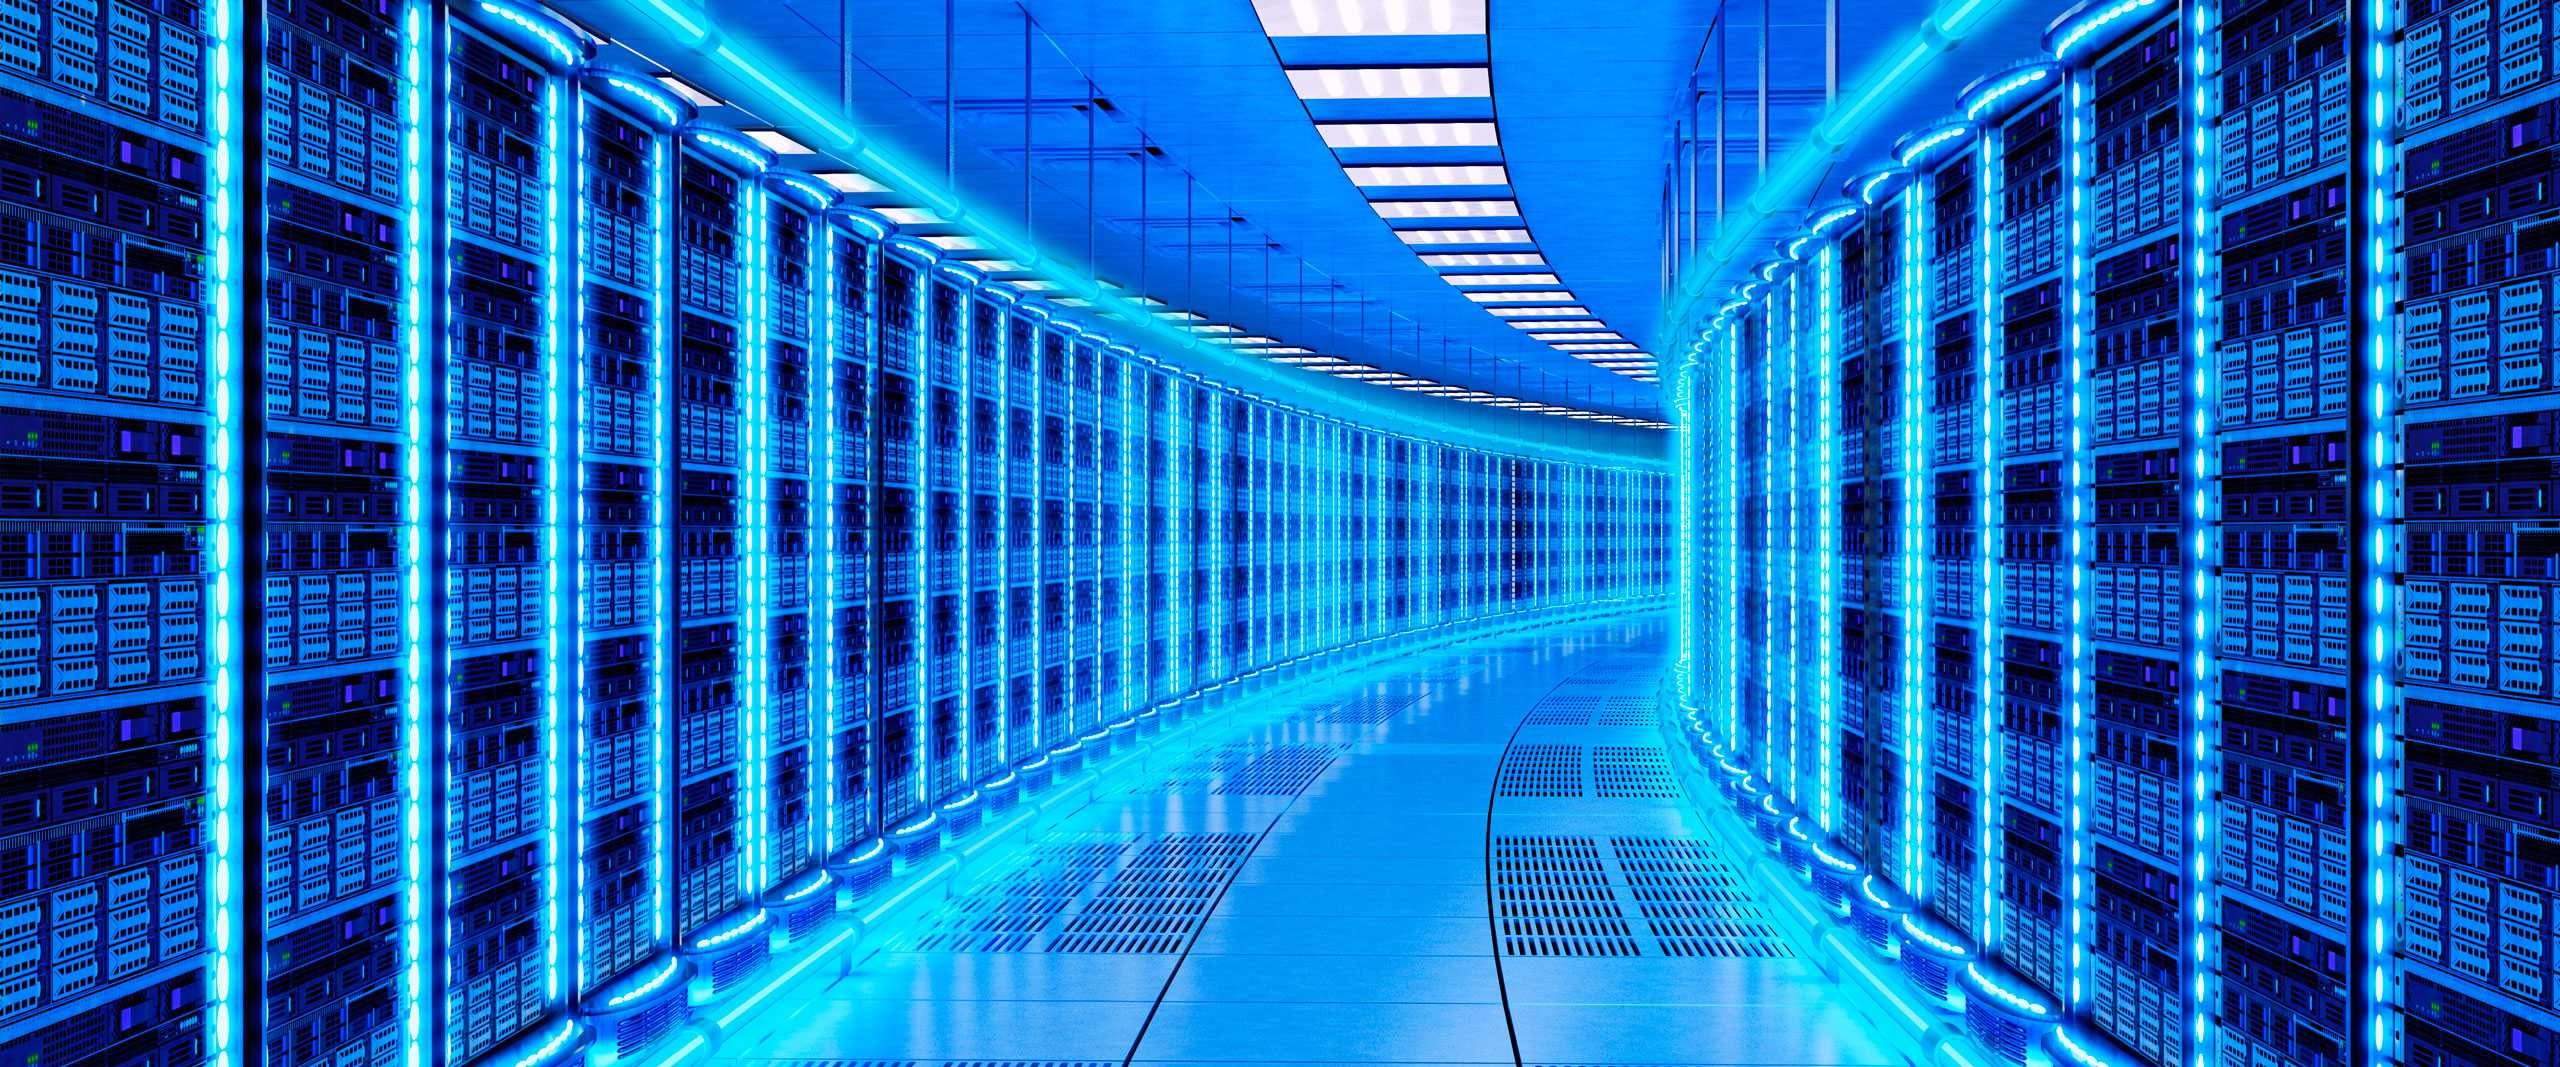
\includegraphics[width=\textwidth]{CPDintro.jpg}}
\end{figure}
En estas salas se dispone del equipamiento informático necesario para realizar todas las tareas antes mencionadas y para garantizar unas condiciones óptimas de trabajo y facilitar el mantenimiento, además, disponen de diversos sistemas de control y seguridad que permita detectar cualquier tipo de incidente que pueda suponer la ralentización de los procesos o incluso la perdida de la información.

El presente trabajo está dirigido al diseño e implementación de uno de esos sistemas de control y seguridad que poseen los CPD. En este primer capítulo se presentarán las motivaciones para su desarrollo y los objetivos de este TFG, así como la metodología de trabajo y la estructura el proyecto.

\section{Motivación del trabajo}
Contado todo lo anterior, podemos ver que estos centros son de vital importancia hoy en día, en el que toda nuestra vida está en la red, almacenada en un disco duro en alguna parte del mundo. Proteger estos lugares es fundamental para todas las partes implicadas, tanto para los usuarios de los datos como para la empresa que los almacena.

Este proyecto surge a raíz de una propuesta lanzada por mi tutor de TFG, Javier Fernández Muñoz, en la que se propone el desarrollo de un sistema para controlar la temperatura de un CPD y tener visión de su interior. 

Lo sugerido inicialmente son factores básicos para la seguridad de estos sitios y que garanticen su correcto funcionamiento, y sin los cuales se correría un riesgo importante y costoso para el propietario.

Partiendo de esta premisa y dado mi interés por ampliar mis conocimientos sobre el desarrollo de software para pequeños dispositivos, decidí embarcarme en este trabajo, inicialmente solo había trabajado con pequeñas placas para hacer sencillos sistemas que encendieran un LED o movieran un motor. Por todo esto, este trabajo me servirá para meterme de lleno en este campo y poder descubrir nuevas formas de desarrollar software que no hemos tratado en el grado.

Además, no solamente cubrirá la idea que tuvimos inicialmente de controlar la temperatura y visión, sino que se desarrollará un sistema completo, dispositivo y aplicación web, para controlar diferentes variables de un CPD, así como para tener visión en tiempo real de su situación. Esta nueva perspectiva, más completa, nos acerca algo más a un sistema que pudiéramos ver en un lugar tan clave como lo son estos.

\section{Objetivos}
El objetivo de este proyecto es desarrollar un dispositivo capaz de monitorizar diversas variables ambientales del interior de un CPD, realizando numerosas mediciones de estas, almacenar los datos recogidos y confeccionar los gráficos oportunos para su buen entendimiento, a la vez que transmitirá imágenes del interior, todo ello en tiempo real.

El dispositivo pretende ser de bajo presupuesto, pero que sea perfectamente capaz de detectar los posibles riesgos y proporcionar una visión general y suficiente del ambiente interior de la sala. Por este motivo no podrá contar con la precisión de equipos de altas capacidades. Su bajo coste posibilitará que pueda ser usado en centros de menor escala o con presupuestos más ajustados.

Como se ha dicho anteriormente los datos recogidos se almacenarán en una base de datos al efecto, que también será creada y gestionada correspondientemente para que pueda ser consultada  en cualquier momento y analizarse en busca de posibles problemas o para mejorar el sistema Paralelamente se desarrollará una página web para permitir el acceso a la información anterior desde cualquier dispositivo con acceso a internet.

Otros objetivos relacionados son:
\begin{itemize}
	\item Acceso a la información de los diferentes dispositivos de medida conectados, para gestionarlos de manera más sencilla.
	      \pagebreak
	      
	\item Base de datos y servidor web siempre accesible en la red, para tener conocimiento de posibles incidentes.
	\item Sistema de seguridad mediante inicio de sesión, para acceder a los datos e imagen tomada.
	\item Página web simple e intuitiva, para facilitar la gestión de la información mostrada.
	\item Página web responsive, para móvil, tablet y ordenador.
\end{itemize}

\section{Metodología}
La metodología que se va a emplear en este proyecto es la conocida Métrica V3 \cite{portal_administracion_electronica_metrica_nodate}, con algunas pequeñas modificaciones para una mejor adaptación al trabajo que vamos a desarrollar.

Emplear una metodología nos permite seguir el ciclo de vida del proyecto en un orden adecuado. Uno de los aspectos más importantes de Métrica V3 es su capacidad para adaptarse a este tipo de proyectos, así como es capaz de tener presente  las necesidades del cliente durante todo el proceso.

Se muestra a continuación en la \autoref{fig:metrica_v3} un diagrama de Métrica V3 elaborado por el Ministerio de Administraciones Públicas para que se pueda entender como es este ciclo:

\begin{figure}[H]
	\ffigbox[\FBwidth]
	{\caption[Diagrama Métrica V3]{Diagrama Métrica V3 \cite{portal_administracion_electronica_metrica_nodate}}
		\label{fig:metrica_v3}}
	{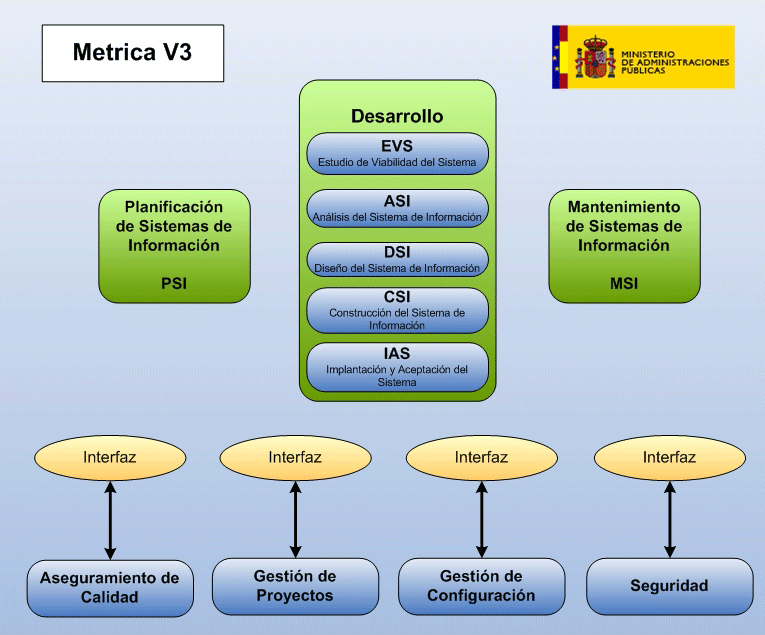
\includegraphics[scale=0.65]{Metrica3.png}}
\end{figure}

\section{Estructura del documento}
En esta sección se presentan los diferentes capítulos que conforman este documento, para que se puedan entender mejor las diferentes fases de Métrica V3 que completan el ciclo de desarrollo del proyecto. 

Capítulos en los que se divide el documento:

\begin{itemize}
	\item \textbf{Introducción (\autoref{ch:introduccion}):} Este capítulo tiene como propósito presentar al lector el tema que se tratará antes de profundizar en él. También se presentan las motivaciones que se han tenido en cuenta para la elección de este tema y los objetivos de este TFG. Por último, se explica la estructura y metodología que sigue el contenido.
	\item \textbf{Estado del arte (\autoref{ch:estado}):} Consiste en un análisis de la situación actual del producto que planeamos desarrollar, buscando soluciones existentes al problema que intentamos solucionar o que sean similares. Después de conocer esas soluciones se buscan los puntos fuertes para intentar mejorarlos y los débiles para solucionarlos, para sacar el mejor producto posible al mercado.
	\item \textbf{Análisis del sistema - ASI (\autoref{ch:analisis}):} Presenta las especificaciones del sistema que el cliente ha solicitado, así como los casos de uso, las diferentes situaciones en las que se podrá interactuar con el mismo. Las especificaciones se recogerán como requisitos de usuario, que tras haber sido analizadas por el analista se completaran y especificaran mejor en forma de requisitos funcionales y no funcionales. Para comprobar que todo ha sido recogido correctamente se verificara con matrices de trazabilidad.
	\item \textbf{Diseño del sistema - DSI (\autoref{ch:diseno}):} Concreta los elementos que conforman el sistema siguiendo las especificaciones detalladas en los componentes, estos elementos son: la arquitectura del sistema, el diagrama de subsistemas y componentes con sus correspondientes definiciones, el modelo de datos que se emplea para almacenar los datos, las interfaces de la aplicación web que visualiza el usuario y el esquema que sigue el hardware del dispositivo. 
	\item \textbf{Implementación - CSI (\autoref{ch:implementacion}):} Detalla cómo se han conectado los diferentes elementos del dispositivo para realizar las diferentes tareas, así como la conexión que se realiza con el servidor para mostrar la información en la aplicación web.
	\item \textbf{Pruebas (\autoref{ch:pruebas}):} Se especifican cuáles serán las pruebas que se realizarán para comprobar que el sistema funciona correctamente, además de garantizar que se cumplen todas las especificaciones marcadas por el cliente en los requisitos del análisis.
	\pagebreak
	
	\item \textbf{Gestión del proyecto - PSI (\autoref{ch:gestion}):} Expone la planificación temporal del proyecto, indicando el tiempo dedicado a cada una de las partes del documento, acompañado del diagrama de Gantt correspondiente. \\ Este capítulo también comprende el presupuesto, en el que se presentan de manera desglosada todos los gastos asociados al proyecto, y finaliza con un resumen en el que se indica el precio final del proyecto para nuestro cliente.
	\item \textbf{Marco regulador (\autoref{ch:marco}):} Recoge los aspectos legales relacionados con el proyecto, con las tecnologías que se han empleado y el impacto de nuestro sistema.
	\item \textbf{Conclusiones (\autoref{ch:conclusiones}):} Es el último capítulo del desarrollo del proyecto, en el que se recoge, tras todo el proceso de diseño e implementación, cuáles son las virtudes de este sistema, así como mi valoración personal sobre el conjunto de este trabajo. \\ Se concluye con una mirada al futuro, con posibles aplicaciones que se le podrán dar y analizando cuáles serían posibles mejoras y funcionalidades para el producto.
	\item \textbf{Bibliografía:} Recoge las referencias a todos los recursos que han sido consultados durante la realización de este documento, con el propósito de dar validez a la información que se ha presentado y si fuera necesario profundizar más en algún punto.
\end{itemize}
\chapter{Estado del arte}
\label{ch:estado}
En este capítulo se presentan de una manera más detallada cuáles son los factores físicos que afectan a la seguridad de los CPD en la actualidad. Después se estudiarán y expondrán cuáles son las alternativas que existen actualmente que hacen algo parecido a lo que pretendemos desarrollar, lo que nos dará una visión general de la situación para desarrollar nuestro sistema. Por último, se analizarán las distintas alternativas de software y hardware para el sistema, escogiendo las que mejor se adapten al mismo.

\section{Seguridad física en los CPD}\label{sec:seguridad_fisica_CPD}
Según los criterios del Instituto Nacional de Ciberseguridad de España (INCIBE) para construir un CPD seguro es necesario tener en cuenta las siguientes áreas \cite{noauthor_pon_2015}:
\begin{itemize}
	\item \textbf{Control de acceso:} Es uno de los aspectos de seguridad más importantes a tener en cuenta, porque nos permite evitar que personas ajenas puedan acceder a estos recintos y hagan un uso indebido de las instalaciones o provoque daños intencionadamente, del mismo modo, se tiene controlado al personal autorizado que pueda entrar en el recinto con intención de perjudicar a la empresa, manteniendo un registro de todos los accesos. Pueden instalarse sistema de acceso por huella digital, verificación de voz, lectores de tarjetas, etc.

	También se debe asegurar que no se pueda acceder a la sala mediante el empleo de la fuerza, con la instalación de puertas blindadas o acorazadas, o sistemas que eviten que las puertas puedan quedar abiertas accidentalmente, mediante el uso de sistemas de alarma si esto ocurre.
	\item \textbf{Seguimiento dentro de la sala:} Como complemento a lo anterior, es conveniente tener conocimiento de todo lo que haga el personal autorizado en el interior de estos recintos en cada momento. Esto se consigue con la instalación de equipos de videovigilancia o un circuito cerrado de televisión (CCTV).
	\item \textbf{Dificultar la identificación del CPD:} Dentro de lo posible es conveniente que el menor número de personas posible tenga conocimiento de la ubicación exacta del CPD, para evitar cualquier manipulación.
	\item \textbf{Medidas contra incendios:} Aparte de estar construidos con materiales resistentes a altas temperaturas o ignífugos, existirán sensores de humo y calor que permiten detectar si se está produciendo un incendio. En cuanto se detecte un incendio, se activará el sistema de extinción por gas, para evitar dañar los equipos. Estos sistemas pasarán revisiones periódicamente para su correcto funcionamiento.
	      \pagebreak
	\item \textbf{Seguridad del cableado:} Se emplea cableado apantallado para evitar acoplamientos o interferencias, además de estar claramente diferenciados según su función, como los de alimentación y de comunicaciones, para facilitar el mantenimiento del CPD.
	\item \textbf{Medidas contra problemas de suministro eléctrico:} Es otro de los sistemas fundamentales en los CPD, que permite mantener el suministro eléctrico necesario para garantizar la disponibilidad del servicio y evitar la pérdida o dañado de los datos y de los propios equipos. Las medidas que se toman a este respecto son la implantación de mecanismos de redundancia eléctrica para que los servidores no pierdan la alimentación eléctrica en caso de un corte de la empresa suministradora, como son los Sistemas de Alimentación Ininterrumpida (SAI) o grupos electrógenos.
	\item \textbf{Suelo y techo técnico:} Este tipo de suelos nos permiten, a la vez que elevar los equipos respecto al nivel original de la sala, distribuir todo el cableado necesario por debajo de él, siendo más fácil el mantenimiento, quedando la sala más limpia y despejada y garantizando una ventilación que evite sobrecalentamientos. El techo técnico permite lo mismo que el suelo, pero con las instalaciones por encima de un falso techo registrable permitiendo a la vez instalar el propio sistema de climatización de la sala. Ambos sistemas son muy importantes para el reducir el consumo de energía empleado para climatizar, hasta en un 45 \% \cite{noauthor_suelo_2020}, además de permitir un constante movimiento del flujo de aire por la sala. Otra función que ofrecen es evitar los daños por inundación.
	\item \textbf{Sistema de climatización:} Se encarga de controlar la temperatura y humedad de la sala regulando el enfriamiento, ventilación, humidificación y flujo de aire. También existen sistemas que mantienen la temperatura idónea de los equipos mediante refrigeración líquida e incluso inmersos en fluidos dieléctricos.
	
	Además, hay sistemas que controlan la calidad del aire y la existencia de gases. Los límites ambientales recomendados internacionalmente son: para la temperatura, entre 18 °C y 27 °C, y para la humedad, entre el 40 \% y el 60 \% \cite{noauthor_recommended_nodate}.
\end{itemize}

\section{Soluciones actuales}
En esta sección se presentarán cuáles son las alternativas que existen actualmente y que tienen el mismo propósito que el sistema que se va a desarrollar en este proyecto.

Como se trata de un sistema de control ambiental y videovigilancia no cubriremos todos los aspectos de seguridad que se han presentado en la \autoref{sec:seguridad_fisica_CPD}, pero sí se desarrollaran: Seguimiento dentro de la sala, Medidas contra incendios y Sistema de climatización.

INCOMPLETO, FALTA ENCONTRARLAS

\section{Critica al Estado del arte}
PUNTOS FUERTES DE CADA UNA

\section{Propuesta}\label{sec:propuesta}
El sistema que se va a desarrollar consistirá en un dispositivo de reducidas dimensiones que dispondrá de una placa y una serie de sensores, que tomaran los datos periódicamente y los enviaran a una base de datos que podrá ser consultada mediante una web.

Este dispositivo constará de las siguientes funcionalidades:
\begin{itemize}
	\item Proporcionar imagen en tiempo real del interior de la sala, que nos permitirá ver lo que ocurre y poder actuar de una manera eficaz ante cualquier circunstancia adversa que lo requiera. La imagen podrá ser vista, aparte de por el personal de seguridad si es que existe en el propio edificio, también por vía IP por la persona o personas encargadas de la misma mediante la clave necesaria.
	\item Controlar la temperatura y humedad ambiental de la sala, para detectar posibles fallos en el sistema de climatización o fugas de agua de instalaciones próximas que puedan provocar la entrada de agua en el recinto.
	\item Detección de incendios mediante el control del nivel de CO y CO$_2$, incluso antes de que pueda llegar a producirse llama, como en el caso de una combustión inicial e incompleta de algunos materiales, que emitirían CO o cuando se haya llegado a producir esta, con la emisión de CO$_2$.
	\item Control de la calidad del aire del recinto, para evitar el deterioro precoz de algunos equipos sensibles a las partículas en suspensión.
\end{itemize}

\section{Estudio de Alternativas de Solución}
En esta sección se presentarán las distintas alternativas que se pueden utilizar para dar solución a cada una de las necesidades planteadas en la \autoref{sec:propuesta}.

\subsection{Alternativas: Placa}\label{subsec:altPlacas}
Para comenzar debemos analizar cuáles son las posibles placas sobre las que podemos desarrollar nuestro dispositivo. Las placas que se buscan deben ser programables y permitirnos instalar una serie de sensores que podamos monitorear, por esta razón se ha decidido evaluar la línea de productos de Raspberry Pi Foundation. 

\begin{figure}[H]
	\ffigbox[\FBwidth]
	{\caption{Logo Raspberry Pi}}
	{\def\svgwidth{.21\textwidth}
		\input{./imagenes/Raspberry_Pi_Logo.eps_tex}}
\end{figure}

Raspberry Pi es una computadora de una sola placa (SBC) de bajo coste, que comenzaron a venderse en 2012 y son las ideales para proyectos de electrónica que requieran de una máquina potente de reducidas de dimensiones. Cuenta con su propio sistema operativo y es capaz de funcionar como un ordenador completo. Todas las versiones incluyen un procesador Broadcom, RAM, GPU, conexión de cámara y 40 pines GPIO (Entrada/Salida de Propósito General), pero no cuentan con memoria interna y debe ser añadida por MicroSD \cite{noauthor_raspberry_2021}.

A continuación se presentan las valoradas para este proyecto, que son el modelo reducido para domótica y los dos modelos más recientes \cite{noauthor_raspberry_nodate}:
\begin{figure}[!htb]
	\minipage{0.32\textwidth}
	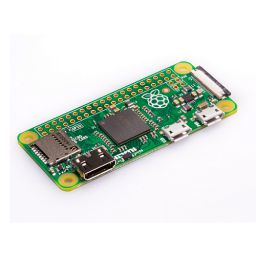
\includegraphics[width=\linewidth]{raspberry-pi-zero.jpg}
	\caption{Raspberry Pi Zero, Raspberry Pi 3 B+ y Raspberry Pi 4 B}
	\endminipage\hfill
	\minipage{0.32\textwidth}
	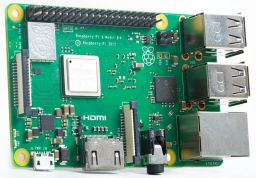
\includegraphics[width=\linewidth]{raspberry-pi-3b-plus.jpg}
	\endminipage\hfill
	\minipage{0.32\textwidth}%
	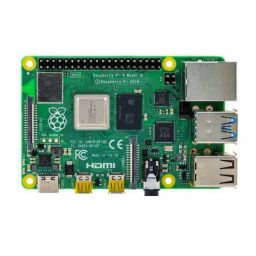
\includegraphics[width=\linewidth]{raspberry-pi-4-b.jpg}
	\endminipage
\end{figure}
\begin{table}[H]
	\centering
	\caption{Comparación gama Raspberry Pi}
	\label{tab:comp_placas}
	\resizebox{\textwidth}{!}{%
		\begin{tabular}{|l|c|c|c|}
			\hline
			                                     & \cellcolor[HTML]{BFBFBF}\textbf{Raspberry Pi Zero} & \cellcolor[HTML]{BFBFBF}\textbf{Raspberry Pi 3 B+} & \cellcolor[HTML]{BFBFBF}\textbf{Raspberry Pi 4 B} \\ \hline
			\cellcolor[HTML]{BFBFBF}CPU          & \begin{tabular}[c]{@{}c@{}}1-GHz, 1-core\\ Broadcom BCM2835\\ (ARM1176JZF-S)\end{tabular}                          & \begin{tabular}[c]{@{}c@{}}1.4-GHz, 4-core\\ Broadcom BCM2837B0\\ (Cortex-A53)\end{tabular}                          & \begin{tabular}[c]{@{}c@{}}1.5-GHz, 4-core\\ Broadcom BCM2711\\ (Cortex-A72)\end{tabular}                         \\ \hline
			\cellcolor[HTML]{BFBFBF}RAM          & \begin{tabular}[c]{@{}c@{}}LPDDR2\\ 512 MB\end{tabular}                          & \begin{tabular}[c]{@{}c@{}}LPDDR2\\ 1 GB\end{tabular}                          & \begin{tabular}[c]{@{}c@{}}LPDDR4\\ 1, 2, 4 GB\end{tabular}                        \\ \hline
			\cellcolor[HTML]{BFBFBF}USB          & 1 Micro                                            & 4 (2.0)                                            & \begin{tabular}[c]{@{}c@{}}2 (2.0)\\ 4 (3.0)\end{tabular}                        \\ \hline
			\cellcolor[HTML]{BFBFBF}Alimentación & microUSB                                           & microUSB                                           & USB Tipo-C                                        \\ \hline
			\cellcolor[HTML]{BFBFBF}HDMI         & MiniHDMI                                           & HDMI                                               & 2 Micro HDMI                                      \\ \hline
			\cellcolor[HTML]{BFBFBF}Ethernet     & No                                                 & Gigabit 300 Mbps                                   & True Gigabit                                      \\ \hline
			\cellcolor[HTML]{BFBFBF}Wi-Fi        & No                                                 & Dual-band Wi-Fi                                    & Dual-band Wi-Fi                                   \\ \hline
			\cellcolor[HTML]{BFBFBF}Bluetooth    & No                                                 & 4.2                                                & 5.0                                               \\ \hline
			\cellcolor[HTML]{BFBFBF}Tamaño       & 65 x 30 mm                                         & 85 x 30 mm                                         & 85 x 30 mm                                        \\ \hline
			\cellcolor[HTML]{BFBFBF}Precio       & 5,4 euros                                          & 39 euros                                           & 39, 61 o 93 euros                                 \\ \hline
		\end{tabular}%
	}
\end{table}

\subsection{Alternativas: Componentes}\label{subsec:altComponentes}
Se estudiarán los diferentes sensores y cámaras que se podrán integrar en el dispositivo, para controlar el estado y ambiente de la sala con la finalidad de mantener la seguridad de los equipos que se encuentra en la misma.

\paragraph{Sensores}\mbox{} \\
Como se explicó en la propuesta se han buscado sensores capaces de captar temperatura, humedad, CO, CO$_2$ y la calidad del aire. A continuación se exponen los sensores que se han encontrado y que cubren estas necesidades. Más adelante decidiremos si se adaptan al proyecto.

Comencemos con el sensor de temperatura y humedad, que es frecuente que ambos aparezcan juntos en el mismo sensor \cite{noauthor_comparing_2019}:

\begin{table}[H]
	\centering
	\caption{Comparación sensores de temperatura y humedad}
	\label{tab:comp_temp}
	\resizebox{\textwidth}{!}{%
		\begin{tabular}{|l|c|c|c|c|c|c|}
			\hline
			                                                   & \cellcolor[HTML]{BFBFBF}\textbf{DHT11}                 & \cellcolor[HTML]{BFBFBF}\textbf{DHT22} & \cellcolor[HTML]{BFBFBF}\textbf{LM35} & \cellcolor[HTML]{BFBFBF}{\color[HTML]{3A3A3A} \textbf{DS18B20}} & \cellcolor[HTML]{BFBFBF}{\color[HTML]{3A3A3A} \textbf{BME280}} & \cellcolor[HTML]{BFBFBF}{\color[HTML]{3A3A3A} \textbf{BMP180}} \\ \hline
			\cellcolor[HTML]{BFBFBF}Temperatura                & Si                                                     & Si                                     & Si                                    & Si                                                              & Si                                                             & Si                                                             \\ \hline
			\cellcolor[HTML]{BFBFBF}Humedad                    & Si                                                     & Si                                     & No                                    & No                                                              & Si                                                             & No                                                             \\ \hline
			\cellcolor[HTML]{BFBFBF}\begin{tabular}[c]{@{}l@{}}Protocolo de\\ comunicación\end{tabular} & 1 cable                                                & 1 cable                                & Analógico                             & 1 cable                                                         & I2C                                                            & I2C                                                            \\ \hline
			\cellcolor[HTML]{BFBFBF}Voltaje                    & 3 - 5.5 V                                              & 3 - 6 V                                & 4 - 30 V                              & 3 - 5.5 V                                                       & \begin{tabular}[c]{@{}c@{}}1.7 - 3.6 V chip\\ 3.3 - 5 V placa\end{tabular}                                     & \begin{tabular}[c]{@{}c@{}}1.8 - 3.6 V chip\\ 3.3 - 5 V placa\end{tabular}                                     \\ \hline
			\cellcolor[HTML]{BFBFBF}\begin{tabular}[c]{@{}l@{}}Rango de\\ temperatura\end{tabular} & 0 - 50ºC                                               & -40 - 80ºC                             & -55 - 150ºC                           & -55 - 125ºC                                                     & -40 - 85ºC                                                     & 0 - 65ºC                                                       \\ \hline
			\cellcolor[HTML]{BFBFBF}\begin{tabular}[c]{@{}l@{}}Precisión de\\ temperatura\end{tabular} & \cellcolor[HTML]{FFFFFF}{\color[HTML]{3A3A3A} +/- 2ºC} & +/- 0.5ºC                              & +/-0.5ºC                              & +/-0.5ºC                                                        & +/-0.5ºC                                                       & +/-0.5ºC                                                       \\ \hline
			\cellcolor[HTML]{BFBFBF}\begin{tabular}[c]{@{}l@{}}Rango de\\ humedad\end{tabular} & 20-80\%                                                & 0-100\%                                & -                                     & -                                                               & 0-100\%                                                        & -                                                              \\ \hline
			\cellcolor[HTML]{BFBFBF}\begin{tabular}[c]{@{}l@{}}Precisión de\\ humedad\end{tabular} & +/- 5\%                                                & +/- 2-5\%                              & -                                     & -                                                               & +/- 4\%                                                        & -                                                              \\ \hline
			\cellcolor[HTML]{BFBFBF}Precio                     & 6,99 euros                                             & 10,99 euros                            & 6,07 euros                            & 0.82 euros                                                      & 7,23 euros                                                     & 2,02 euros                                                     \\ \hline
		\end{tabular}%
	}
\end{table}

Para el sensor de monóxido de carbono (CO) no se encontraron muchas posibilidades, por lo que se ha optado por el MQ7, cuyas especificaciones son las siguientes.

\minipage{0.45\textwidth}
\begin{figure}[H]
	\caption{Sensor MQ-7}
	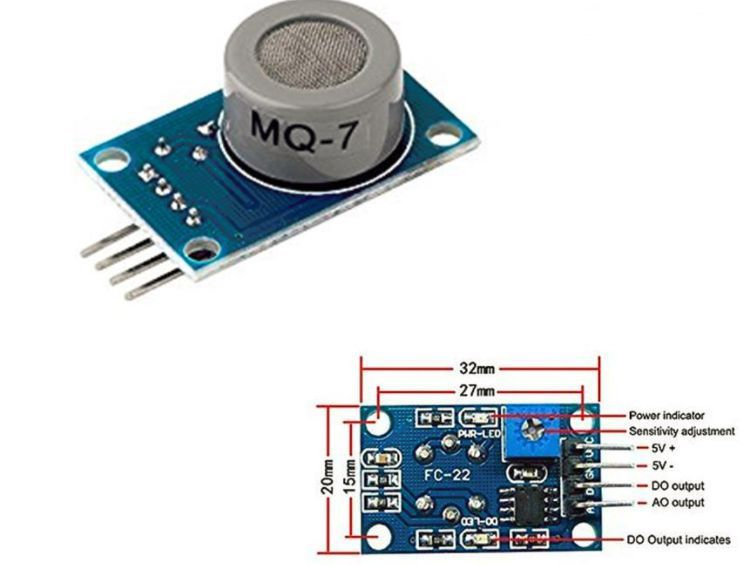
\includegraphics[width=\linewidth]{mq7.jpg}
\end{figure}
\endminipage\hfill
\minipage{0.45\textwidth}
\begin{table}[H]
	\centering
	\caption{Especificaciones módulo MQ-7}
	\label{tab:mq_7}
	\begin{tabular}{|
		>{\columncolor[HTML]{BFBFBF}}l |l|}
		\hline
		\textbf{Alimentación}               & 5 V                        \\ \hline
		\textbf{Intensidad}                 & 140 m                      \\ \hline
		\textbf{Tipo}                       & Analógico                  \\ \hline
		\textbf{Precalentamiento}           & 20 s                       \\ \hline
		\textbf{\begin{tabular}[c]{@{}l@{}}Tiempo de\\ respuesta\end{tabular}} & 1 ms                       \\ \hline
		\textbf{Pines}                      & \begin{tabular}[c]{@{}l@{}}GND\\ DOUT\\ AOUT\\ VCC\end{tabular} \\ \hline
		\textbf{Rango}                      & 10 -10.000 ppm             \\ \hline
		\textbf{Tamaño}                     & 40x20 mm                   \\ \hline
	\end{tabular}
\end{table}
\endminipage

\pagebreak
A continuación se muestran los sensores de dióxido de carbono (CO$_2$) que se han considerado para este proyecto.

\begin{table}[H]
	\centering
	\caption{Comparación sensores CO$_2$}
	\label{tab:comp_co2}
	\resizebox{\textwidth}{!}{%
		\begin{tabular}{|l|c|c|c|c|}
			\hline
			                                                   & \cellcolor[HTML]{BFBFBF}\textbf{MH-Z14A} & \cellcolor[HTML]{BFBFBF}\textbf{CCS811} & \cellcolor[HTML]{BFBFBF}\textbf{S8 LP} & \cellcolor[HTML]{BFBFBF}\textbf{MG-811} \\ \hline
			\cellcolor[HTML]{BFBFBF}Voltaje                    & 4.5 - 5,5 V                              & 3,3 - 5 V                               & 4.5 - 5,25 V                           & 5 V                                     \\ \hline
			\cellcolor[HTML]{BFBFBF}Rango                      & 0 - 10.000 ppm                           & 400 - 29.206 ppm                        & 400 - 2.000 ppm                        & 0 - 10.000 ppm                          \\ \hline
			\cellcolor[HTML]{BFBFBF}\begin{tabular}[c]{@{}l@{}}Protocolo de\\ comunicación\end{tabular} & UART                                     & I2C                                     & UART                                   & Analógico                               \\ \hline
		\end{tabular}%
	}
\end{table}

Por último, antes de pasar a la parte de videovigilancia, se muestran las especificaciones del módulo de calidad de aire que se ha considerado más adecuado. En este caso no se muestran varias posibilidades dada la escasa variedad de módulos que solo incorporen este tipo de sensor. Todos los encontrados eran parte de sistemas mucho más complejos que eran capaces de funcionar de manera independiente. Se ha escogido el módulo SDS011 que es capaz de medir la materia particulada (PM) de 2,5 y 10 micrómetros, cuyas características son las siguientes \cite{noauthor_nova_nodate}:

\minipage{0.45\textwidth}
\begin{figure}[H]
	\caption{Sensor SDS011}
	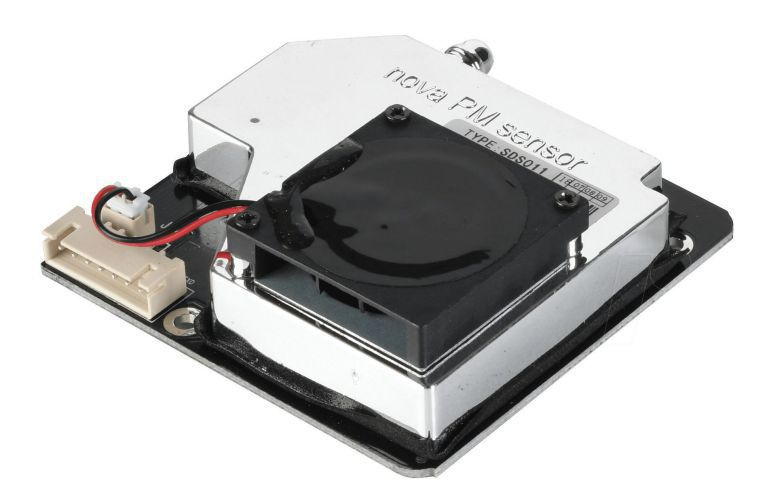
\includegraphics[width=\linewidth]{SDS011.jpg}
\end{figure}
\endminipage\hfill
\minipage{0.45\textwidth}
\begin{table}[H]
	\centering
	\caption{Especificaciones módulo SDS011}
	\label{tab:sds011}
	\resizebox{\linewidth}{!}{%
		\begin{tabular}{|
			>{\columncolor[HTML]{BFBFBF}}l |l|}
			\hline
			\textbf{Voltaje}             & 5 V                                                        \\ \hline
			\textbf{Corriente máxima}    & 100 mA                                                     \\ \hline
			\textbf{Rango}               & 0 - 999.9 ug/m3                                            \\ \hline
			\textbf{Resolución}          & 0,3 ug/m3                                                  \\ \hline
			\textbf{Error relativo}      & 10 \%                                                      \\ \hline
			\textbf{Tiempo de respuesta} & 1 s                                                        \\ \hline
			\textbf{Salida}              & UART (USB)                                                 \\ \hline
			\textbf{Tamaño}              & \cellcolor[HTML]{FFFFFF}{\color[HTML]{656D78} 71x70x23 mm} \\ \hline
		\end{tabular}%
	}
\end{table}
\endminipage

\pagebreak
\paragraph{Cámaras}\mbox{} \\
Las cámaras que se presentan a continuación han sido buscadas con la intención de que sean compatibles con la Raspberry Pi, por lo que su conexión debe ser mediante la CSI de la placa. Se han propuesto una serie de cámaras con diferentes categorías \cite{cholewiak_raspberry_2017}, algunas cuentan con una mejor resolución, angular o ambos. Aun así las cuatro cámaras tienen los mismos modos de grabación: 1080p30, 720p60 y 640×480p60/90.

\begin{table}[H]
	\centering
	\caption{Comparación de módulos cámara}
	\label{tab:comp_camara}
	\resizebox{\textwidth}{!}{%
		\begin{tabular}{|l|c|c|c|c|}
			\hline
			                                                   & \cellcolor[HTML]{BFBFBF}\textbf{\begin{tabular}[c]{@{}c@{}}Raspberry Pi\\ Camera\end{tabular}}        & \cellcolor[HTML]{BFBFBF}\textbf{\begin{tabular}[c]{@{}c@{}}Raspberry Pi v2\\ Camera\end{tabular}} & \cellcolor[HTML]{BFBFBF}\textbf{\begin{tabular}[c]{@{}c@{}}Waveshare RPi\\ Camera (I)\end{tabular}}        & \cellcolor[HTML]{BFBFBF}\textbf{Sony IMX477}                       \\ \hline
			\cellcolor[HTML]{BFBFBF}Megapíxeles                & 5                                                                  & 8                                                           & 5                                                                  & 12.3                                                               \\ \hline
			\cellcolor[HTML]{BFBFBF}FOV                        & 54°                                                                & 62.2°                                                       & 170°                                                               & Depende de la lente                                                \\ \hline
			\cellcolor[HTML]{BFBFBF}\begin{tabular}[c]{@{}l@{}}Resolución\\ del sensor\end{tabular} & \cellcolor[HTML]{FFFFFF}{\color[HTML]{2A2A2A} 2592 × 1944 pixeles} & 3280 × 2464 pixeles                                         & \cellcolor[HTML]{FFFFFF}{\color[HTML]{2A2A2A} 2592 × 1944 pixeles} & \cellcolor[HTML]{FFFFFF}{\color[HTML]{2A2A2A} 4056 x 3040 pixeles} \\ \hline
			\cellcolor[HTML]{BFBFBF}Precio                     & 19,70 euros                                                        & 24,95 euros                                                 & 28,01 euros                                                        & 50 euros                                                           \\ \hline
		\end{tabular}%
	}
\end{table}

\section{Hardware y Software seleccionado}\label{sec:hardwareSoftware}
En esta sección se escogerá una solución de entre las expuestas en las subsecciones antes descritas.

\subsection{Placa}
Entre las tres placas que se han valorado, aunque la Zero está más pensada para dispositivos ligeros y compactos, se ha decidido descartarla por sus reducidas capacidades y la falta de wifi o ethernet que requerirían un módulo extra para obtener conexión a internet. Entre las dos restantes se ha optado por la Raspberry Pi 3B+, porque ante la similitud de características de las placas y su coste, esta tenía más disponibilidad en el mercado y el suministro era más rápido. 
\begin{figure}[H]
	\ffigbox[\FBwidth]
	{\caption{Esquema de Raspberry Pi 3 B+}}
	{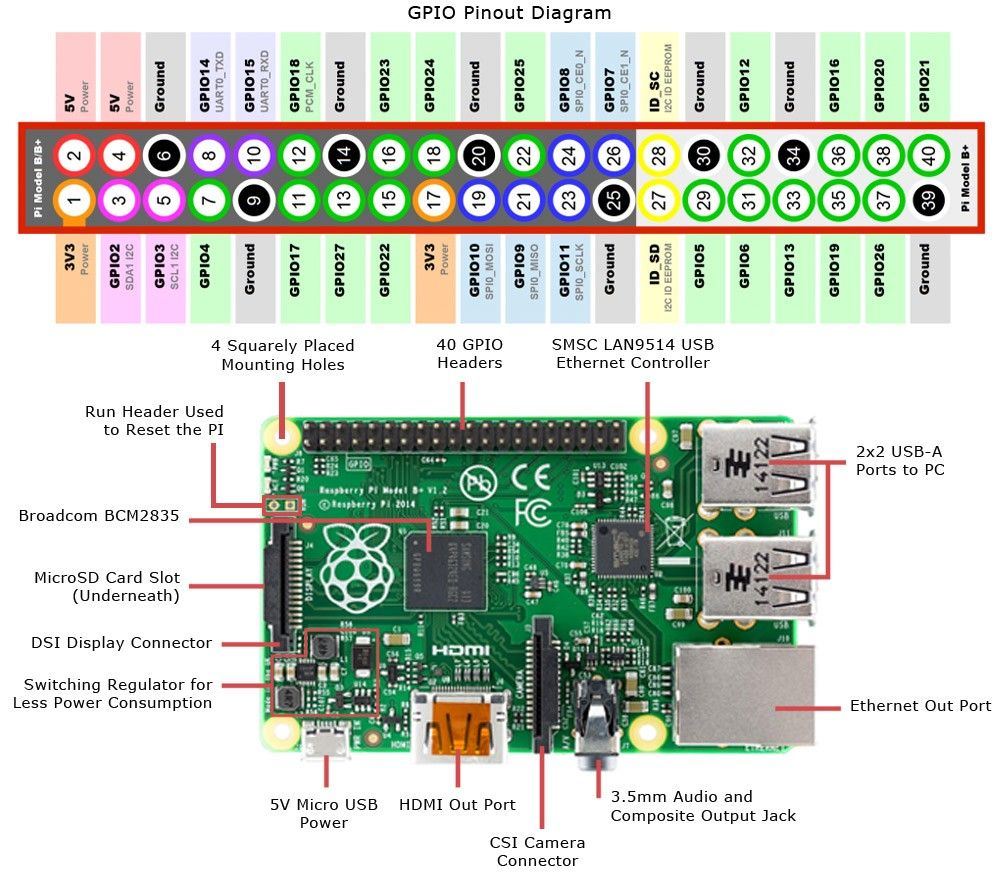
\includegraphics[scale=0.35]{esquema-raspberry-pi-3b-plus.jpg}}
\end{figure}
En cuanto al sistema operativo que se emplea en esta placa, se ha decidido utilizar Raspbian que es una distribución de Linux basado en Debian que está altamente optimizada para estas placas, además por tratarse de un sistema operativo que es conocido por el programador que llevara a cabo el desarrollo.

\subsection{Componentes}
El sensor de temperatura y humedad que se ha elegido como la mejor opción ha sido el DHT11. Por un precio reducido es capaz de medir tanto temperatura como humedad, ambas en el rango en el que se mueven las medidas en un CPD (18 °C - 27 °C y  40 \% - 60 \%) con una precisión aceptable. La decisión por el DHT11 y no el DHT22 ha sido que tiene un mayor coste y supera, con mucho, las temperaturas que se medirían, desaprovechando sus capacidades.
\begin{figure}[H]
	\ffigbox[\FBwidth]
	{\caption{Sensor DHT11}}
	{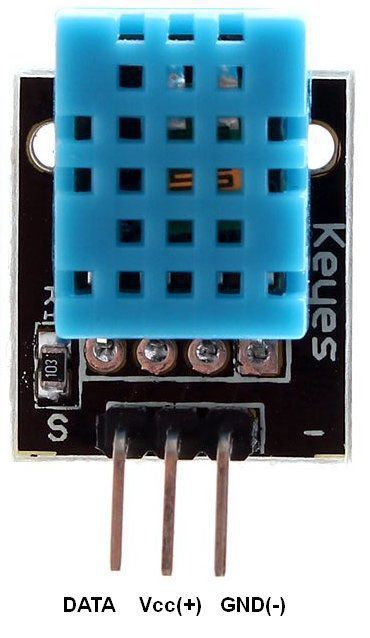
\includegraphics[scale=0.35]{dht11.jpg}}
\end{figure}
El sensor de CO$_2$ por el que nos hemos decantado ha sido el MH-Z14A, que ante unas capacidades similares al MG-811 se ha preferido el protocolo de comunicación UART. Por otro lado el CCS811 a pesar de tener muy buenas características su rango comienza demasiado arriba para captar la concentración atmosférica común, cosa que el MH-Z14A si capta y su cota más alta es suficiente para este proyecto.
\begin{figure}[H]
	\ffigbox[\FBwidth]
	{\caption{Sensor MH-Z14A}}
	{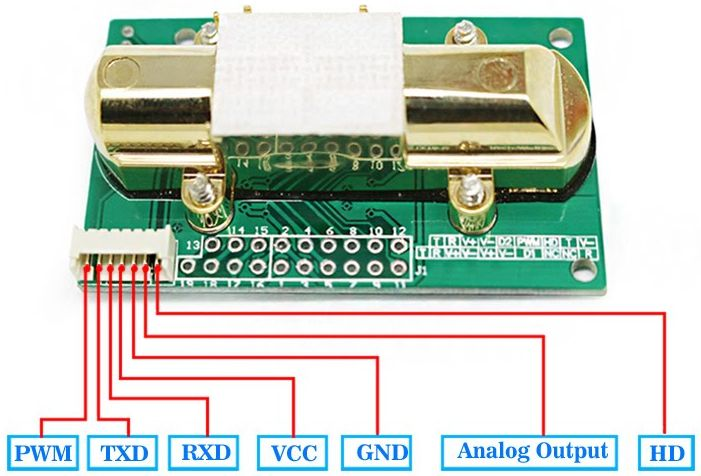
\includegraphics[scale=0.4]{MH-Z14A.jpg}}
\end{figure}
Con respecto al sensor de CO y al de calidad el aire, se ha escogido el MQ-7 y SDS011 por la falta de variedad y disponibilidad en esta clase de sensores, pero esto no ha hecho que se hayan escogido componentes de peor calidad o que no vayan a desempeñar su función adecuadamente.

En cuanto a la cámara, tras analizar las especificaciones de las candidatas, se ha decidido que la que mejor se adapta al proyecto es la Raspberry Pi Camera. Se ha seleccionado esta cámara dado que todas ellas graban con las mismas resoluciones y frecuencias de cuadros, y como se trata de un dispositivo orientado a videovigilancia no buscamos que la resolución de las fotos sea la mejor, sino que pueda proporcionar una buena imagen a tiempo real por un bajo coste. Además el angular de la Raspberry Pi Camera es suficiente para captar lo que se encuentra dentro de la sala.
\begin{figure}[H]
	\ffigbox[\FBwidth]
	{\caption{Modulo Raspberry Pi Camera}}
	{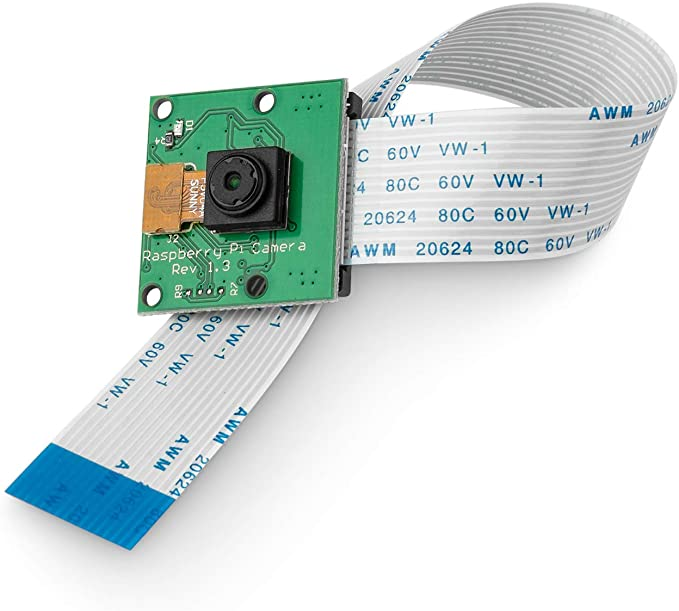
\includegraphics[scale=0.35]{Raspberry-Pi-Camera-Module-Rev-1.3.jpg}}
\end{figure}

\subsection{Lenguajes de programación}
En esta subsección se expondrán los lenguajes que se emplearán tanto para el desarrollo del dispositivo como para la parte web del proyecto. Los lenguajes han sido escogidos en función del conocimiento del programador que lo llevara a cabo, estos lenguajes son PHP para la web y Python para el dispositivo.

\paragraph{PHP}\mbox{} \\
\begin{figure}[H]
	\ffigbox[\FBwidth]
	{\caption{Logo PHP}}
	{
\includegraphics[scale=0.08]{phplogo.jpg}}
\end{figure}
PHP (Hypertext Preprocessor) \cite{welling_php_2003} es un lenguaje de programación para desarrollo web de código abierto desde el lado del servidor, creado originalmente en 1994 por Rasmus Lerdorf, aunque hoy en día es producido por The PHP Group. Este lenguaje puede ser embebido en una página HTML para que se ejecute cada vez que sea visualizado, el código en este lenguaje es interpretado por el servidor para convertirlo en otro lenguaje de salida.

Es el más utilizado en toda la red en abril de 2021 \cite{noauthor_usage_nodate} con un 79 \% de uso en los sitios web de los que se conoce el lenguaje del lado del servidor en 2021.

Para desarrollar la web se utilizará el editor de código fuente Visual Studio Code, editor multiplataforma de código abierto creado por Microsoft en 2015 \cite{noauthor_visual_2021} que dispone de infinidad de extensiones para facilitar el desarrollo en cualquier lenguaje de programación.

\paragraph{Python}\mbox{} \\
\begin{figure}[H]
	\ffigbox[\FBwidth]
	{\caption{Logo Python}}
	{
\includegraphics[scale=0.1]{Python-logo.jpg}}
\end{figure}
Python es un lenguaje de programación de alto nivel interpretado desarrollado por la Python Software Foundation en 1991 \cite{montoro_python_2012}, cuya intención es facilitar la legibilidad del código haciendo la programación más accesible para todo el mundo. Su uso ha aumentado mucho en la última década llegando a ser uno de los lenguajes de propósito general más extendidos, puede ser utilizado para multitud de propósitos a diferencia de muchos otros lenguajes que se centran en un área específica.

Para programar todo el comportamiento del dispositivo se empleará este lenguaje por su sencillez y utilidad, el IDE que empleara el programador será PyCharm Professional edition creado por JetBrains en 2010 \cite{noauthor_pycharm_2021} al que se tiene acceso gracias a la licencia de estudiante, aunque también hay una edición gratuita llamada Community edition.

Se ha decidido el uso de este, en vez de emplear también Visual Studio Code, al estar orientado al desarrollo de programas en Python y por la posibilidad de conectarse vía SSH con la Raspberry Pi para sincronizar los programas y facilitar el proceso.

\subsection{Servidor y Base de datos}\label{subsec:servidorDB}
\begin{figure}[H]
	\ffigbox[\FBwidth]
	{\caption{Logo XAMPP}}
	{
\includegraphics[scale=0.13]{xampp.png}}
\end{figure}
El servidor que se va a emplear para este proyecto será Apache \cite{noauthor_apache_nodate}, uno de los servidores de código abierto más utilizados que nos permite alojar y ser propietarios de nuestra propia web.

En cuanto a la base de datos utilizaremos MariaDB \cite{noauthor_mariadb_nodate} que es un software de código abierto derivado y compatible con MySQL, que actualmente es de Oracle y de pago, pero mantiene la esencia de este gestor de base de datos.

Todo esto se orquestará mediante XAMPP una herramienta de software libre multiplataforma \cite{noauthor_xampp_nodate} que nos permite crear el servidor y base de datos alojada por nosotros mismos. Este software nos ofrece desde un mismo sitio lanzar nuestra base de datos MariaDB, el servidor web Apache y los intérpretes de PHP y Perl.
\chapter{Análisis del sistema}
\label{ch:analisis}
En este capítulo se explica de qué es capaz el producto desarrollado. Comienza con una descripción del sistema de una manera detallada, a continuación se extraerán los requisitos de usuario y casos de uso, lo que nos permite hacernos una idea clara de lo que necesita el sistema y así poder conceptualizarlo en forma de requisitos de software. En último lugar, se establece la relación entre los requisitos de usuario y los de software en una matriz de trazabilidad, pudiendo así comprobar que todas las peticiones del usuario han sido tenidas en cuenta.

Además, este capítulo sirve como base para los siguientes, como son el de Diseño (\autoref{ch:diseno}) y el de Implementación (\autoref{ch:implementacion}), en los que basándose en los requisitos recogidos se empezara a dar forma al sistema.

\section{Definición del Sistema}
El propósito de este proyecto es desarrollar un dispositivo que nos proporcione videovigilancia y medidas de diferentes factores ambientales, para garantizar la seguridad de un CPD. Las diferentes medidas que se tomen se almacenaran para poder ser consultadas junto con la imagen de videovigilancia a través de una plataforma web.
\begin{figure}[H]
	\ffigbox[\FBwidth]
	{\caption{Diagrama del sistema}
		\label{fig:diagrama_sistema}}
	{\tikzset{every picture/.style={line width=0.75pt}} %set default line width to 0.75pt        
	
	\begin{tikzpicture}[x=0.75pt,y=0.75pt,yscale=-1,xscale=1]
		
		\draw   (82.49,90) .. controls (82.49,78.95) and (98.16,70) .. (117.49,70) .. controls (136.82,70) and (152.49,78.95) .. (152.49,90) .. controls (152.49,101.05) and (136.82,110) .. (117.49,110) .. controls (98.16,110) and (82.49,101.05) .. (82.49,90) -- cycle ;
		
		\draw   (320,60) -- (530,60) -- (530,200) -- (320,200) -- cycle ;
		\draw   (440,108) .. controls (440,96.95) and (455.67,88) .. (475,88) .. controls (494.33,88) and (510,96.95) .. (510,108) .. controls (510,119.05) and (494.33,128) .. (475,128) .. controls (455.67,128) and (440,119.05) .. (440,108) -- cycle ;
		
		\draw   (275,140.5) -- (275,179.5) .. controls (275,185.3) and (261.57,190) .. (245,190) .. controls (228.43,190) and (215,185.3) .. (215,179.5) -- (215,140.5)(275,140.5) .. controls (275,146.3) and (261.57,151) .. (245,151) .. controls (228.43,151) and (215,146.3) .. (215,140.5) .. controls (215,134.7) and (228.43,130) .. (245,130) .. controls (261.57,130) and (275,134.7) .. (275,140.5) -- cycle ;
		
		\draw   (210,77) .. controls (210,73.13) and (213.13,70) .. (217,70) -- (273,70) .. controls (276.87,70) and (280,73.13) .. (280,77) -- (280,103) .. controls (280,106.87) and (276.87,110) .. (273,110) -- (217,110) .. controls (213.13,110) and (210,106.87) .. (210,103) -- cycle ;
		
		\draw   (340,117) .. controls (340,113.13) and (343.13,110) .. (347,110) -- (403,110) .. controls (406.87,110) and (410,113.13) .. (410,117) -- (410,143) .. controls (410,146.87) and (406.87,150) .. (403,150) -- (347,150) .. controls (343.13,150) and (340,146.87) .. (340,143) -- cycle ;
		
		\draw   (440,152) .. controls (440,140.95) and (455.67,132) .. (475,132) .. controls (494.33,132) and (510,140.95) .. (510,152) .. controls (510,163.05) and (494.33,172) .. (475,172) .. controls (455.67,172) and (440,163.05) .. (440,152) -- cycle ;
		
		\draw    (440,152) -- (411.92,143.57) ;
		\draw [shift={(410,143)}, rotate = 376.7] [color={rgb, 255:red, 0; green, 0; blue, 0 }  ][line width=0.75]    (10.93,-3.29) .. controls (6.95,-1.4) and (3.31,-0.3) .. (0,0) .. controls (3.31,0.3) and (6.95,1.4) .. (10.93,3.29)   ;
		\draw    (440,108) -- (411.86,119.26) ;
		\draw [shift={(410,120)}, rotate = 338.2] [color={rgb, 255:red, 0; green, 0; blue, 0 }  ][line width=0.75]    (10.93,-3.29) .. controls (6.95,-1.4) and (3.31,-0.3) .. (0,0) .. controls (3.31,0.3) and (6.95,1.4) .. (10.93,3.29)   ;
		\draw    (152.49,90) -- (208,90.24) ;
		\draw [shift={(210,90.25)}, rotate = 180.25] [color={rgb, 255:red, 0; green, 0; blue, 0 }  ][line width=0.75]    (10.93,-3.29) .. controls (6.95,-1.4) and (3.31,-0.3) .. (0,0) .. controls (3.31,0.3) and (6.95,1.4) .. (10.93,3.29)   ;
		\draw    (340,120) -- (281.79,90.89) ;
		\draw [shift={(280,90)}, rotate = 386.57] [color={rgb, 255:red, 0; green, 0; blue, 0 }  ][line width=0.75]    (10.93,-3.29) .. controls (6.95,-1.4) and (3.31,-0.3) .. (0,0) .. controls (3.31,0.3) and (6.95,1.4) .. (10.93,3.29)   ;
		\draw    (340,140) -- (281.9,159.37) ;
		\draw [shift={(280,160)}, rotate = 341.57] [color={rgb, 255:red, 0; green, 0; blue, 0 }  ][line width=0.75]    (10.93,-3.29) .. controls (6.95,-1.4) and (3.31,-0.3) .. (0,0) .. controls (3.31,0.3) and (6.95,1.4) .. (10.93,3.29)   ;
		\draw    (245,130) -- (245,112) ;
		\draw [shift={(245,110)}, rotate = 450] [color={rgb, 255:red, 0; green, 0; blue, 0 }  ][line width=0.75]    (10.93,-3.29) .. controls (6.95,-1.4) and (3.31,-0.3) .. (0,0) .. controls (3.31,0.3) and (6.95,1.4) .. (10.93,3.29)   ;
		\draw   (190,60) -- (300,60) -- (300,200) -- (190,200) -- cycle ;
		\draw   (74.97,170) .. controls (74.97,158.95) and (94.01,150) .. (117.49,150) .. controls (140.97,150) and (160,158.95) .. (160,170) .. controls (160,181.05) and (140.97,190) .. (117.49,190) .. controls (94.01,190) and (74.97,181.05) .. (74.97,170) -- cycle ;
		
		\draw    (160.2,170) -- (212.2,170) ;
		\draw [shift={(214.2,170)}, rotate = 180] [color={rgb, 255:red, 0; green, 0; blue, 0 }  ][line width=0.75]    (10.93,-3.29) .. controls (6.95,-1.4) and (3.31,-0.3) .. (0,0) .. controls (3.31,0.3) and (6.95,1.4) .. (10.93,3.29)   ;
		\draw    (120,150) -- (208.23,103.93) ;
		\draw [shift={(210,103)}, rotate = 512.4300000000001] [color={rgb, 255:red, 0; green, 0; blue, 0 }  ][line width=0.75]    (10.93,-3.29) .. controls (6.95,-1.4) and (3.31,-0.3) .. (0,0) .. controls (3.31,0.3) and (6.95,1.4) .. (10.93,3.29)   ;
		
		\draw (321,202) node [anchor=north west][inner sep=0.75pt]  [font=\footnotesize] [align=left] {Dispositivo};
		\draw (222,150.43) node [anchor=north west][inner sep=0.75pt]   [align=left] {\begin{minipage}[lt]{32.65pt}\setlength\topsep{0pt}
				\begin{center}
					{\footnotesize Base de}\\{\footnotesize Datos}
				\end{center}
				
			\end{minipage}};
		\draw (232,84) node [anchor=north west][inner sep=0.75pt]  [font=\footnotesize] [align=left] {Web};
		\draw (191,202) node [anchor=north west][inner sep=0.75pt]  [font=\footnotesize] [align=left] {Servidor};
		\draw (95.99,84) node [anchor=north west][inner sep=0.75pt]  [font=\footnotesize] [align=left] {Usuario};
		\draw (359,124) node [anchor=north west][inner sep=0.75pt]  [font=\footnotesize] [align=left] {Placa};
		\draw (448.5,102) node [anchor=north west][inner sep=0.75pt]  [font=\footnotesize] [align=left] {Sensores};
		\draw (452.5,146) node [anchor=north west][inner sep=0.75pt]  [font=\footnotesize] [align=left] {Cámara};
		\draw (79.49,164) node [anchor=north west][inner sep=0.75pt]  [font=\footnotesize] [align=left] {Administrador};
		
	\end{tikzpicture}}
\end{figure}

Como se puede ver en la \autoref{fig:diagrama_sistema} el sistema consistirá en:
\begin{itemize}
	\item \textbf{Usuario:} Será el personal autorizado encargado de controlar las imágenes que proporcione la cámara y revisar las mediciones que transmitan los sensores del dispositivo.
	\item \textbf{Administrador:} Persona encargada del mantenimiento de la Base de Datos y de la web, así como de la buena recepción de las mediciones y de las imágenes. Ante cualquier incidencia es el responsable de resolverla.
	\item \textbf{Web:} Página donde se puede acceder a los diferentes dispositivos, sus medidas e imagen de video.
	\item \textbf{Base de Datos:} Almacén de la información de los usuarios, la de los dispositivos y las mediciones que recogen.
	\item \textbf{Servidor:} Lugar accesible para el usuario donde se alojan la web y la base de datos.
	\item \textbf{Placa:} Dispositivo donde se implantan los distintos sensores y la cámara.
	\item \textbf{Sensores:} Dispositivos sensibles a los diferentes factores ambientales que se medirán en el CPD.
	\item \textbf{Cámara:} Dispositivo que captura la imagen que se utilizara para la videovigilancia.
	\item \textbf{Dispositivo:} Conjunto de la placa, los sensores y la cámara.
\end{itemize}

\section{Requisitos de usuario}
En esta sección se recogen todas exigencias que el cliente nos solicita para este proyecto, en forma de requisitos de usuario, que serán mostrados según la \autoref{tab:plantilla_ru}.
\begin{table}[H]
	\centering
	\caption{Plantilla de los Requisitos de Usuario}
	\label{tab:plantilla_ru}
	\begin{tabular}{|l|p{.77\textwidth}|}
		\hline
		\multicolumn{2}{|c|}{\cellcolor[HTML]{BFBFBF}{\color[HTML]{000000} \textbf{RU-XX}}} \\ \hline
		\textbf{Nombre}      &   \\ \hline
		\textbf{Descripción} &   \\ \hline
		\textbf{Prioridad}   &   \\ \hline
		\textbf{Necesidad}   &   \\ \hline
		\textbf{Fuente}      &   \\ \hline
		\textbf{Versión}     &   \\ \hline
	\end{tabular}
\end{table}
\begin{itemize}
	\item \textbf{RU-XX:} Identificador del Requisito de Usuario, el XX tomará un valor en función de la posición.
	\item \textbf{Nombre:} Nombre representativo del asunto del requisito.
	\item \textbf{Descripción:} Exposición más detallada del requisito.
	\item \textbf{Prioridad:} Indica si debe ser considerado desde el principio o si, por el contrario, puede retrasarse. Puede ser: Alta, Mediana o Baja.
	\item \textbf{Necesidad:} Importancia del requisito sobre el sistema, pudiendo ser: Esencial, Deseable u Opcional.
	\item \textbf{Fuente:} Procedencia del requisito.
	\item \textbf{Versión:} Indica si ha sufrido variaciones a lo largo del tiempo.
\end{itemize}

Los requisitos de usuario son los siguientes:
\newcount\ru
\ru=1
\begin{table}[H]
	\caption{RU-0\number\ru}
	\begin{tabular}{|l|p{.77\textwidth}|}
		\hline
		\multicolumn{2}{|c|}{\cellcolor[HTML]{BFBFBF}{\color[HTML]{000000} \textbf{RU-0\number\ru}}} \\ \hline
		\textbf{Nombre}      & Medir la temperatura                                                                                          \\ \hline
		\textbf{Descripción} & El dispositivo debe contar con un sensor capaz medir la temperatura de la sala entre los valores establecidos \\ \hline
		\textbf{Prioridad}   & Alta                                                                                                          \\ \hline
		\textbf{Necesidad}   & Esencial                                                                                                      \\ \hline
		\textbf{Fuente}      & Cliente                                                                                                       \\ \hline
		\textbf{Versión}     & 1.0                                                                                                           \\ \hline
	\end{tabular}
\end{table}
\advance\ru by 1
\begin{table}[H]
	\caption{RU-0\number\ru}
	\begin{tabular}{|l|p{.77\textwidth}|}
		\hline
		\multicolumn{2}{|c|}{\cellcolor[HTML]{BFBFBF}{\color[HTML]{000000} \textbf{RU-0\number\ru}}} \\ \hline
		\textbf{Nombre}      & Medir la humedad                                                                                          \\ \hline
		\textbf{Descripción} & El dispositivo debe contar con un sensor capaz medir la humedad de la sala entre los valores establecidos \\ \hline
		\textbf{Prioridad}   & Alta                                                                                                      \\ \hline
		\textbf{Necesidad}   & Esencial                                                                                                  \\ \hline
		\textbf{Fuente}      & Cliente                                                                                                   \\ \hline
		\textbf{Versión}     & 1.0                                                                                                       \\ \hline
	\end{tabular}
\end{table}
\advance\ru by 1
\begin{table}[H]
	\caption{RU-0\number\ru}
	\begin{tabular}{|l|p{.77\textwidth}|}
		\hline
		\multicolumn{2}{|c|}{\cellcolor[HTML]{BFBFBF}{\color[HTML]{000000} \textbf{RU-0\number\ru}}} \\ \hline
		\textbf{Nombre}      & Medir el CO                                                                                                           \\ \hline
		\textbf{Descripción} & El dispositivo debe contar con un sensor capaz medir el monóxido de carbono de la sala entre los valores establecidos \\ \hline
		\textbf{Prioridad}   & Media                                                                                                                 \\ \hline
		\textbf{Necesidad}   & Deseable                                                                                                              \\ \hline
		\textbf{Fuente}      & Cliente                                                                                                               \\ \hline
		\textbf{Versión}     & 1.0                                                                                                                   \\ \hline
	\end{tabular}
\end{table}
\advance\ru by 1
\begin{table}[H]
	\caption{RU-0\number\ru}
	\begin{tabular}{|l|p{.77\textwidth}|}
		\hline
		\multicolumn{2}{|c|}{\cellcolor[HTML]{BFBFBF}{\color[HTML]{000000} \textbf{RU-0\number\ru}}} \\ \hline
		\textbf{Nombre}      & Medir el CO$_2$                                                                                                      \\ \hline
		\textbf{Descripción} & El dispositivo debe contar con un sensor capaz medir el dióxido de carbono de la sala entre los valores establecidos \\ \hline
		\textbf{Prioridad}   & Media                                                                                                                \\ \hline
		\textbf{Necesidad}   & Deseable                                                                                                             \\ \hline
		\textbf{Fuente}      & Cliente                                                                                                              \\ \hline
		\textbf{Versión}     & 1.0                                                                                                                  \\ \hline
	\end{tabular}
\end{table}
\advance\ru by 1
\begin{table}[H]
	\caption{RU-0\number\ru}
	\begin{tabular}{|l|p{.77\textwidth}|}
		\hline
		\multicolumn{2}{|c|}{\cellcolor[HTML]{BFBFBF}{\color[HTML]{000000} \textbf{RU-0\number\ru}}} \\ \hline
		\textbf{Nombre}      & Medir la calidad del aire                                                                                           \\ \hline
		\textbf{Descripción} & El dispositivo debe contar con un sensor capaz medir la calidad del aire de la sala para el correcto funcionamiento \\ \hline
		\textbf{Prioridad}   & Media                                                                                                               \\ \hline
		\textbf{Necesidad}   & Deseable                                                                                                            \\ \hline
		\textbf{Fuente}      & Cliente                                                                                                             \\ \hline
		\textbf{Versión}     & 1.0                                                                                                                 \\ \hline
	\end{tabular}
\end{table}
\advance\ru by 1
\begin{table}[H]
	\caption{RU-0\number\ru}
	\begin{tabular}{|l|p{.77\textwidth}|}
		\hline
		\multicolumn{2}{|c|}{\cellcolor[HTML]{BFBFBF}{\color[HTML]{000000} \textbf{RU-0\number\ru}}} \\ \hline
		\textbf{Nombre}      & Videovigilancia                                                              \\ \hline
		\textbf{Descripción} & El dispositivo debe captar la imagen del interior de la sala en todo momento \\ \hline
		\textbf{Prioridad}   & Alta                                                                         \\ \hline
		\textbf{Necesidad}   & Esencial                                                                     \\ \hline
		\textbf{Fuente}      & Cliente                                                                      \\ \hline
		\textbf{Versión}     & 1.0                                                                          \\ \hline
	\end{tabular}
\end{table}
\advance\ru by 1
\begin{table}[H]
	\caption{RU-0\number\ru}
	\begin{tabular}{|l|p{.77\textwidth}|}
		\hline
		\multicolumn{2}{|c|}{\cellcolor[HTML]{BFBFBF}{\color[HTML]{000000} \textbf{RU-0\number\ru}}} \\ \hline
		\textbf{Nombre}      & Conectividad                                            \\ \hline
		\textbf{Descripción} & El dispositivo debe tener conexión inalámbrica a la red \\ \hline
		\textbf{Prioridad}   & Alta                                                    \\ \hline
		\textbf{Necesidad}   & Esencial                                                \\ \hline
		\textbf{Fuente}      & Cliente                                                 \\ \hline
		\textbf{Versión}     & 1.0                                                     \\ \hline
	\end{tabular}
\end{table}
\advance\ru by 1
\begin{table}[H]
	\caption{RU-0\number\ru}
	\begin{tabular}{|l|p{.77\textwidth}|}
		\hline
		\multicolumn{2}{|c|}{\cellcolor[HTML]{BFBFBF}{\color[HTML]{000000} \textbf{RU-0\number\ru}}} \\ \hline
		\textbf{Nombre}      & Bajo consumo                                        \\ \hline
		\textbf{Descripción} & El dispositivo debe tener un bajo consumo eléctrico \\ \hline
		\textbf{Prioridad}   & Media                                               \\ \hline
		\textbf{Necesidad}   & Deseable                                            \\ \hline
		\textbf{Fuente}      & Cliente                                             \\ \hline
		\textbf{Versión}     & 1.0                                                 \\ \hline
	\end{tabular}
\end{table}
\advance\ru by 1
\begin{table}[H]
	\caption{RU-0\number\ru}
	\begin{tabular}{|l|p{.77\textwidth}|}
		\hline
		\multicolumn{2}{|c|}{\cellcolor[HTML]{BFBFBF}{\color[HTML]{000000} \textbf{RU-0\number\ru}}} \\ \hline
		\textbf{Nombre}      & Histórico de medidas                            \\ \hline
		\textbf{Descripción} & Se deben almacenar todas las medidas realizadas \\ \hline
		\textbf{Prioridad}   & Alta                                            \\ \hline
		\textbf{Necesidad}   & Esencial                                        \\ \hline
		\textbf{Fuente}      & Cliente                                         \\ \hline
		\textbf{Versión}     & 1.0                                             \\ \hline
	\end{tabular}
\end{table}
\advance\ru by 1
\begin{table}[H]
	\caption{RU-\number\ru}
	\begin{tabular}{|l|p{.77\textwidth}|}
		\hline
		\multicolumn{2}{|c|}{\cellcolor[HTML]{BFBFBF}{\color[HTML]{000000} \textbf{RU-\number\ru}}} \\ \hline
		\textbf{Nombre}      & Frecuencia de las medidas                                                \\ \hline
		\textbf{Descripción} & El dispositivo debe realizar las medidas con la mayor frecuencia posible \\ \hline
		\textbf{Prioridad}   & Media                                                                    \\ \hline
		\textbf{Necesidad}   & Deseable                                                                 \\ \hline
		\textbf{Fuente}      & Cliente                                                                  \\ \hline
		\textbf{Versión}     & 1.0                                                                      \\ \hline
	\end{tabular}
\end{table}
\advance\ru by 1
\begin{table}[H]
	\caption{RU-\number\ru}
	\begin{tabular}{|l|p{.77\textwidth}|}
		\hline
		\multicolumn{2}{|c|}{\cellcolor[HTML]{BFBFBF}{\color[HTML]{000000} \textbf{RU-\number\ru}}} \\ \hline
		\textbf{Nombre}      & Conexión con la web                                                                          \\ \hline
		\textbf{Descripción} & El dispositivo debe ser capaz de transmitir las medidas e imagen para que se vean  en la web \\ \hline
		\textbf{Prioridad}   & Media                                                                                        \\ \hline
		\textbf{Necesidad}   & Esencial                                                                                     \\ \hline
		\textbf{Fuente}      & Cliente                                                                                      \\ \hline
		\textbf{Versión}     & 1.0                                                                                          \\ \hline
	\end{tabular}
\end{table}
\advance\ru by 1
\begin{table}[H]
	\caption{RU-\number\ru}
	\begin{tabular}{|l|p{.77\textwidth}|}
		\hline
		\multicolumn{2}{|c|}{\cellcolor[HTML]{BFBFBF}{\color[HTML]{000000} \textbf{RU-\number\ru}}} \\ \hline
		\textbf{Nombre}      & Registro en la web                                                                                \\ \hline
		\textbf{Descripción} & El usuario debe solicitar al administrador del sistema que le conceda unas credenciales de acceso \\ \hline
		\textbf{Prioridad}   & Alta                                                                                              \\ \hline
		\textbf{Necesidad}   & Esencial                                                                                          \\ \hline
		\textbf{Fuente}      & Cliente                                                                                           \\ \hline
		\textbf{Versión}     & 1.0                                                                                               \\ \hline
	\end{tabular}
\end{table}
\advance\ru by 1
\begin{table}[H]
	\caption{RU-\number\ru}
	\begin{tabular}{|l|p{.77\textwidth}|}
		\hline
		\multicolumn{2}{|c|}{\cellcolor[HTML]{BFBFBF}{\color[HTML]{000000} \textbf{RU-\number\ru}}} \\ \hline
		\textbf{Nombre}      & Inicio de sesión                                                                                        \\ \hline
		\textbf{Descripción} & El usuario para acceder a la web debe aportar un usuario y contraseña que se le ha asignado previamente \\ \hline
		\textbf{Prioridad}   & Alta                                                                                                    \\ \hline
		\textbf{Necesidad}   & Esencial                                                                                                \\ \hline
		\textbf{Fuente}      & Cliente                                                                                                 \\ \hline
		\textbf{Versión}     & 1.0                                                                                                     \\ \hline
	\end{tabular}
\end{table}
\advance\ru by 1
\begin{table}[H]
	\caption{RU-\number\ru}
	\begin{tabular}{|l|p{.77\textwidth}|}
		\hline
		\multicolumn{2}{|c|}{\cellcolor[HTML]{BFBFBF}{\color[HTML]{000000} \textbf{RU-\number\ru}}} \\ \hline
		\textbf{Nombre}      & Seguridad de la contraseña                                                 \\ \hline
		\textbf{Descripción} & La contraseña se debe almacenar de manera segura ante posibles intrusiones \\ \hline
		\textbf{Prioridad}   & Media                                                                      \\ \hline
		\textbf{Necesidad}   & Deseable                                                                   \\ \hline
		\textbf{Fuente}      & Cliente                                                                    \\ \hline
		\textbf{Versión}     & 1.0                                                                        \\ \hline
	\end{tabular}
\end{table}
\advance\ru by 1
\begin{table}[H]
	\caption{RU-\number\ru}
	\begin{tabular}{|l|p{.77\textwidth}|}
		\hline
		\multicolumn{2}{|c|}{\cellcolor[HTML]{BFBFBF}{\color[HTML]{000000} \textbf{RU-\number\ru}}} \\ \hline
		\textbf{Nombre}      & Lista de dispositivos                                                                                   \\ \hline
		\textbf{Descripción} & Cuando el usuario este dentro de su cuenta podrá ver los diferentes dispositivos a los que tiene acceso \\ \hline
		\textbf{Prioridad}   & Baja                                                                                                    \\ \hline
		\textbf{Necesidad}   & Opcional                                                                                                \\ \hline
		\textbf{Fuente}      & Cliente                                                                                                 \\ \hline
		\textbf{Versión}     & 1.0                                                                                                     \\ \hline
	\end{tabular}
\end{table}
\advance\ru by 1
\begin{table}[H]
	\caption{RU-\number\ru}
	\begin{tabular}{|l|p{.77\textwidth}|}
		\hline
		\multicolumn{2}{|c|}{\cellcolor[HTML]{BFBFBF}{\color[HTML]{000000} \textbf{RU-\number\ru}}} \\ \hline
		\textbf{Nombre}      & Cerrar sesión                        \\ \hline
		\textbf{Descripción} & El usuario podrá salir de su cuenta. \\ \hline
		\textbf{Prioridad}   & Alta                                 \\ \hline
		\textbf{Necesidad}   & Esencial                             \\ \hline
		\textbf{Fuente}      & Cliente                              \\ \hline
		\textbf{Versión}     & 1.0                                  \\ \hline
	\end{tabular}
\end{table}
\advance\ru by 1
\begin{table}[H]
	\caption{RU-\number\ru}
	\begin{tabular}{|l|p{.77\textwidth}|}
		\hline
		\multicolumn{2}{|c|}{\cellcolor[HTML]{BFBFBF}{\color[HTML]{000000} \textbf{RU-\number\ru}}} \\ \hline
		\textbf{Nombre}      & Verificar nombre de usuario                                                          \\ \hline
		\textbf{Descripción} & Al acceder el usuario podrá ver su nombre de usuario para comprobar que es su cuenta \\ \hline
		\textbf{Prioridad}   & Baja                                                                                 \\ \hline
		\textbf{Necesidad}   & Opcional                                                                             \\ \hline
		\textbf{Fuente}      & Cliente                                                                              \\ \hline
		\textbf{Versión}     & 1.0                                                                                  \\ \hline
	\end{tabular}
\end{table}
\advance\ru by 1
\begin{table}[H]
	\caption{RU-\number\ru}
	\begin{tabular}{|l|p{.77\textwidth}|}
		\hline
		\multicolumn{2}{|c|}{\cellcolor[HTML]{BFBFBF}{\color[HTML]{000000} \textbf{RU-\number\ru}}} \\ \hline
		\textbf{Nombre}      & Colores de la web                                                                                   \\ \hline
		\textbf{Descripción} & La web debe estar diseñada en colores no estridentes para que se puedan ver bien en cualquier lugar \\ \hline
		\textbf{Prioridad}   & Alta                                                                                                \\ \hline
		\textbf{Necesidad}   & Deseable                                                                                            \\ \hline
		\textbf{Fuente}      & Cliente                                                                                             \\ \hline
		\textbf{Versión}     & 1.0                                                                                                 \\ \hline
	\end{tabular}
\end{table}
\advance\ru by 1
\begin{table}[H]
	\caption{RU-\number\ru}
	\begin{tabular}{|l|p{.77\textwidth}|}
		\hline
		\multicolumn{2}{|c|}{\cellcolor[HTML]{BFBFBF}{\color[HTML]{000000} \textbf{RU-\number\ru}}} \\ \hline
		\textbf{Nombre}      & Acceso a la web                                                                   \\ \hline
		\textbf{Descripción} & La web debe poder ser accesible desde cualquier dispositivo con acceso a internet \\ \hline
		\textbf{Prioridad}   & Alta                                                                              \\ \hline
		\textbf{Necesidad}   & Esencial                                                                          \\ \hline
		\textbf{Fuente}      & Cliente                                                                           \\ \hline
		\textbf{Versión}     & 1.0                                                                               \\ \hline
	\end{tabular}
\end{table}
\advance\ru by 1
\begin{table}[H]
	\caption{RU-\number\ru}
	\begin{tabular}{|l|p{.77\textwidth}|}
		\hline
		\multicolumn{2}{|c|}{\cellcolor[HTML]{BFBFBF}{\color[HTML]{000000} \textbf{RU-\number\ru}}} \\ \hline
		\textbf{Nombre}      & Página de dispositivo                                                     \\ \hline
		\textbf{Descripción} & Cuando se accede a un dispositivo se mostrará la imagen y medidas tomadas \\ \hline
		\textbf{Prioridad}   & Alta                                                                      \\ \hline
		\textbf{Necesidad}   & Esencial                                                                  \\ \hline
		\textbf{Fuente}      & Cliente                                                                   \\ \hline
		\textbf{Versión}     & 1.0                                                                       \\ \hline
	\end{tabular}
\end{table}
\advance\ru by 1
\begin{table}[H]
	\caption{RU-\number\ru}
	\begin{tabular}{|l|p{.77\textwidth}|}
		\hline
		\multicolumn{2}{|c|}{\cellcolor[HTML]{BFBFBF}{\color[HTML]{000000} \textbf{RU-\number\ru}}} \\ \hline
		\textbf{Nombre}      & Imagen de la cámara                                                                            \\ \hline
		\textbf{Descripción} & La imagen de la cámara debe ser tomada en todo momento, mientras el dispositivo esté conectado \\ \hline
		\textbf{Prioridad}   & Alta                                                                                           \\ \hline
		\textbf{Necesidad}   & Esencial                                                                                       \\ \hline
		\textbf{Fuente}      & Cliente                                                                                        \\ \hline
		\textbf{Versión}     & 1.0                                                                                            \\ \hline
	\end{tabular}
\end{table}
\advance\ru by 1
\begin{table}[H]
	\caption{RU-\number\ru}
	\begin{tabular}{|l|p{.77\textwidth}|}
		\hline
		\multicolumn{2}{|c|}{\cellcolor[HTML]{BFBFBF}{\color[HTML]{000000} \textbf{RU-\number\ru}}} \\ \hline
		\textbf{Nombre}      & Navegar entre las medidas                                                                                                   \\ \hline
		\textbf{Descripción} & Cuando se está en una página de dispositivo, el usuario, debe poder moverse con facilidad entre todos los datos registrados \\ \hline
		\textbf{Prioridad}   & Media                                                                                                                       \\ \hline
		\textbf{Necesidad}   & Deseable                                                                                                                    \\ \hline
		\textbf{Fuente}      & Cliente                                                                                                                     \\ \hline
		\textbf{Versión}     & 1.0                                                                                                                         \\ \hline
	\end{tabular}
\end{table}
\advance\ru by 1
\begin{table}[H]
	\caption{RU-\number\ru}
	\begin{tabular}{|l|p{.77\textwidth}|}
		\hline
		\multicolumn{2}{|c|}{\cellcolor[HTML]{BFBFBF}{\color[HTML]{000000} \textbf{RU-\number\ru}}} \\ \hline
		\textbf{Nombre}      & Medidas tomadas                                                                                      \\ \hline
		\textbf{Descripción} & Los datos que tome el dispositivo deben mostrarse en varios formatos para facilitar su entendimiento \\ \hline
		\textbf{Prioridad}   & Baja                                                                                                 \\ \hline
		\textbf{Necesidad}   & Deseable                                                                                             \\ \hline
		\textbf{Fuente}      & Cliente                                                                                              \\ \hline
		\textbf{Versión}     & 1.0                                                                                                  \\ \hline
	\end{tabular}
\end{table}
\advance\ru by 1
\pagebreak

\section{Casos de uso}
En la \autoref{fig:diagrama_casos_uso} que se muestra a continuación se resumen todos los casos de uso del sistema.

\begin{figure}[H]
	\ffigbox[\textwidth]
	{\caption{Diagrama de Casos de Uso}
		\label{fig:diagrama_casos_uso}}
	{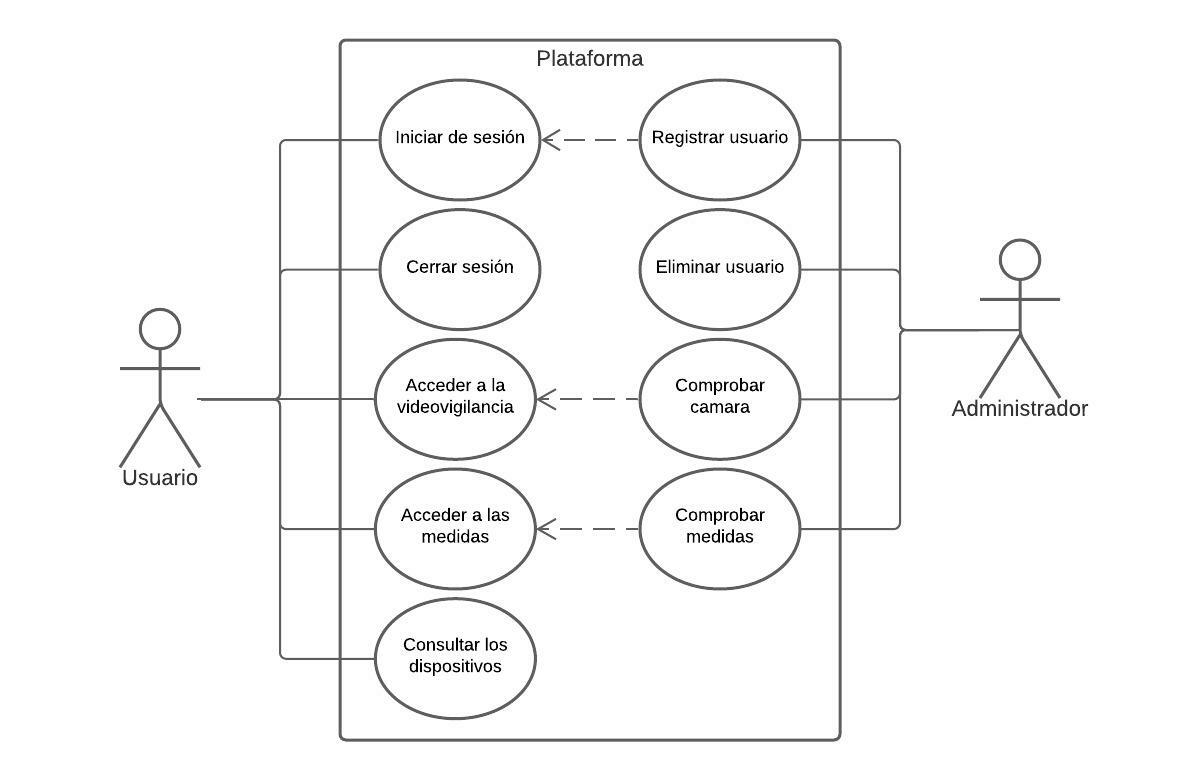
\includegraphics[width=\textwidth]{casos-de-uso.jpeg}}
\end{figure}

Para realizar una descripción más detallada de los casos de uso, empleamos la representación tabular que se muestra en la \autoref{tab:plantilla_cu}.
\begin{table}[H]
	\centering
	\caption{Plantilla de los Casos de Uso}
	\label{tab:plantilla_cu}
	\begin{tabular}{|l|p{.75\textwidth}|}
		\hline
		\multicolumn{2}{|c|}{\cellcolor[HTML]{BFBFBF}{\color[HTML]{000000} \textbf{CU-XX}}} \\ \hline
		\textbf{Caso de uso}     &   \\ \hline
		\textbf{Actores}         &   \\ \hline
		\textbf{Descripción}     &   \\ \hline
		\textbf{Precondiciones}  &   \\ \hline
		\textbf{Postcondiciones} &   \\ \hline
	\end{tabular}
\end{table}

\begin{itemize}
	\item \textbf{CU-XX:} Identificador del caso de uso, el XX tomará un valor en función del orden de este.
	\item \textbf{Caso de uso:} Nombre que identifica el caso de uso.
	\item \textbf{Actores:} Partes implicadas en el caso de uso.
	\item \textbf{Descripción:} Breve exposición de la situación.
	\item \textbf{Precondiciones:} Condiciones que se deben cumplir para que tenga lugar el caso de uso.
	\item \textbf{Postcondiciones:} Que ocurre si se cumple el caso de uso.
\end{itemize}

Ahora que entendemos el significado de cada una de las casillas se procede a detallar los casos de uso.
\newcount\cu
\cu=1
\begin{table}[H]
	\centering
	\caption{CU-0\number\cu}
	\begin{tabular}{|l|p{.75\textwidth}|}
		\hline
		\multicolumn{2}{|c|}{\cellcolor[HTML]{BFBFBF}{\color[HTML]{000000} \textbf{CU-0\number\cu}}} \\ \hline
		\textbf{Caso de uso}     & Registrar usuario                                          \\ \hline
		\textbf{Actores}         & Administrador                                              \\ \hline
		\textbf{Descripción}     & Crear un usuario y contraseña para acceder a la plataforma \\ \hline
		\textbf{Precondiciones}  & Acceder a la página de administración de la BBDD           \\ \hline
		\textbf{Postcondiciones} & Generación de usuario y contraseña de acceso               \\ \hline
	\end{tabular}
\end{table}
\advance\cu by 1
\begin{table}[H]
	\centering
	\caption{CU-0\number\cu}
	\begin{tabular}{|l|p{.75\textwidth}|}
		\hline
		\multicolumn{2}{|c|}{\cellcolor[HTML]{BFBFBF}{\color[HTML]{000000} \textbf{CU-0\number\cu}}} \\ \hline
		\textbf{Caso de uso}     & Eliminar usuario                                 \\ \hline
		\textbf{Actores}         & Administrador                                    \\ \hline
		\textbf{Descripción}     & Revocar el acceso a la plataforma                \\ \hline
		\textbf{Precondiciones}  & Acceder a la página de administración de la BBDD \\ \hline
		\textbf{Postcondiciones} & Registro de la tabla ‘user’ eliminado            \\ \hline
	\end{tabular}
\end{table}
\advance\cu by 1
\begin{table}[H]
	\centering
	\caption{CU-0\number\cu}
	\begin{tabular}{|l|p{.75\textwidth}|}
		\hline
		\multicolumn{2}{|c|}{\cellcolor[HTML]{BFBFBF}{\color[HTML]{000000} \textbf{CU-0\number\cu}}} \\ \hline
		\textbf{Caso de uso}     & Comprobar medidas                                                                         \\ \hline
		\textbf{Actores}         & Administrador                                                                             \\ \hline
		\textbf{Descripción}     & Consultar las medidas, ver que los valores sean razonables y que se reciben continuamente \\ \hline
		\textbf{Precondiciones}  & Poseer usuario y clave de acceso de la BBDD                                               \\ \hline
		\textbf{Postcondiciones} & El administrador ha verificado que funciona correctamente                                 \\ \hline
	\end{tabular}
\end{table}
\advance\cu by 1
\begin{table}[H]
	\centering
	\caption{CU-0\number\cu}
	\begin{tabular}{|l|p{.75\textwidth}|}
		\hline
		\multicolumn{2}{|c|}{\cellcolor[HTML]{BFBFBF}{\color[HTML]{000000} \textbf{CU-0\number\cu}}} \\ \hline
		\textbf{Caso de uso}     & Comprobar cámara                                          \\ \hline
		\textbf{Actores}         & Administrador                                             \\ \hline
		\textbf{Descripción}     & Comprobar que la imagen de la cámara se ve y se actualiza \\ \hline
		\textbf{Precondiciones}  & Poseer usuario y clave de acceso a la web                 \\ \hline
		\textbf{Postcondiciones} & El administrador ha verificado que funciona correctamente \\ \hline
	\end{tabular}
\end{table}
\advance\cu by 1
\begin{table}[H]
	\centering
	\caption{CU-0\number\cu}
	\begin{tabular}{|l|p{.75\textwidth}|}
		\hline
		\multicolumn{2}{|c|}{\cellcolor[HTML]{BFBFBF}{\color[HTML]{000000} \textbf{CU-0\number\cu}}} \\ \hline
		\textbf{Caso de uso}     & Iniciar sesión                          \\ \hline
		\textbf{Actores}         & Usuario                                 \\ \hline
		\textbf{Descripción}     & Acceder a la aplicación                 \\ \hline
		\textbf{Precondiciones}  & El usuario y contraseña está registrado \\ \hline
		\textbf{Postcondiciones} & El usuario accede a la plataforma       \\ \hline
	\end{tabular}
\end{table}
\advance\cu by 1
\begin{table}[H]
	\centering
	\caption{CU-0\number\cu}
	\begin{tabular}{|l|p{.75\textwidth}|}
		\hline
		\multicolumn{2}{|c|}{\cellcolor[HTML]{BFBFBF}{\color[HTML]{000000} \textbf{CU-0\number\cu}}} \\ \hline
		\textbf{Caso de uso}     & Cerrar sesión                                                   \\ \hline
		\textbf{Actores}         & Usuario                                                         \\ \hline
		\textbf{Descripción}     & El usuario termina de consultar las medidas y sale de su cuenta \\ \hline
		\textbf{Precondiciones}  & El usuario ha iniciado sesión                                   \\ \hline
		\textbf{Postcondiciones} & El usuario vuelve a la pantalla de inicio de sesión             \\ \hline
	\end{tabular}
\end{table}
\advance\cu by 1
\begin{table}[H]
	\centering
	\caption{CU-0\number\cu}
	\begin{tabular}{|l|p{.75\textwidth}|}
		\hline
		\multicolumn{2}{|c|}{\cellcolor[HTML]{BFBFBF}{\color[HTML]{000000} \textbf{CU-0\number\cu}}} \\ \hline
		\textbf{Caso de uso}     & Consultar los dispositivos                                \\ \hline
		\textbf{Actores}         & Usuario                                                   \\ \hline
		\textbf{Descripción}     & Visualizar los diferentes dispositivos conectados         \\ \hline
		\textbf{Precondiciones}  & El usuario ha iniciado sesión                             \\ \hline
		\textbf{Postcondiciones} & El usuario visualiza los dispositivos, su estado y nombre \\ \hline
	\end{tabular}
\end{table}
\advance\cu by 1
\begin{table}[H]
	\centering
	\caption{CU-0\number\cu}
	\begin{tabular}{|l|p{.75\textwidth}|}
		\hline
		\multicolumn{2}{|c|}{\cellcolor[HTML]{BFBFBF}{\color[HTML]{000000} \textbf{CU-0\number\cu}}} \\ \hline
		\textbf{Caso de uso}     & Acceder a las medidas                                                                             \\ \hline
		\textbf{Actores}         & Usuario                                                                                           \\ \hline
		\textbf{Descripción}     & Consultar las diferentes medidas tomadas por el dispositivo                                       \\ \hline
		\textbf{Precondiciones}  & El usuario ha iniciado sesión y selecciona un dispositivo                                         \\ \hline
		\textbf{Postcondiciones} & El usuario accede a una página con las gráficas de las medidas y la tabla de histórico de medidas \\ \hline
	\end{tabular}
\end{table}
\advance\cu by 1
\begin{table}[H]
	\centering
	\caption{CU-0\number\cu}
	\begin{tabular}{|l|p{.75\textwidth}|}
		\hline
		\multicolumn{2}{|c|}{\cellcolor[HTML]{BFBFBF}{\color[HTML]{000000} \textbf{CU-0\number\cu}}} \\ \hline
		\textbf{Caso de uso}     & Acceder a la videovigilancia                                            \\ \hline
		\textbf{Actores}         & Usuario                                                                 \\ \hline
		\textbf{Descripción}     & Consultar la imagen de la cámara                                        \\ \hline
		\textbf{Precondiciones}  & El usuario ha iniciado sesión y selecciona un dispositivo               \\ \hline
		\textbf{Postcondiciones} & El usuario accede a una página con la imagen de la cámara a tiempo real \\ \hline
	\end{tabular}
\end{table}

\section{Requisitos de software}
Los requisitos de software descritos en esta sección se basan en los requisitos de usuario proporcionados por el cliente y los casos de uso asociados al sistema. La plantilla que se sigue es la definida por la \autoref{tab:plantilla_rf_rn}.
\begin{table}[H]
	\caption{Plantilla de los Requisitos Funcionales y No funcionales}
	\label{tab:plantilla_rf_rn}
	\begin{tabular}{|l|p{.77\textwidth}|}
		\hline
		\multicolumn{2}{|c|}{\cellcolor[HTML]{BFBFBF}{\color[HTML]{000000} \textbf{ID-XX}}} \\ \hline
		\textbf{Nombre}      &   \\ \hline
		\textbf{Descripción} &   \\ \hline
		\textbf{Prioridad}   &   \\ \hline
		\textbf{Necesidad}   &   \\ \hline
		\textbf{Fuente}      &   \\ \hline
		\textbf{Versión}     &   \\ \hline
	\end{tabular}
\end{table}
\begin{itemize}
	\item \textbf{ID-XX:} Identifica los requisitos mediante la siguiente codificación: ID será RF si es un requisito funcional o RN si es un requisito no funcional y XX tomará un valor en función de la posición.
	\item \textbf{Nombre:} Nombre representativo del asunto del requisito.
	\item \textbf{Descripción:} Exposición más detallada del requisito.
	\item \textbf{Prioridad:} Indica si debe ser considerado desde el principio o si, por el contrario, puede retrasarse. Puede ser: Alta, Mediana o Baja.
	\item \textbf{Necesidad:} Importancia del requisito sobre el sistema, pudiendo ser: Esencial, Deseable u Opcional.
	\item \textbf{Fuente:} Procedencia del requisito.
	\item \textbf{Versión:} Indica si ha sufrido variaciones a lo largo del tiempo.
\end{itemize}

Tras esta explicación de la plantilla en las siguientes subsecciones se presentan los requisitos funcionales y no funcionales.
\subsection{Requisitos Funcionales}
\newcount\rf
\rf=1
\begin{table}[H]
	\caption{RF-0\number\rf}
	\begin{tabular}{|l|p{.77\textwidth}|}
		\hline
		\multicolumn{2}{|c|}{\cellcolor[HTML]{BFBFBF}{\color[HTML]{000000} \textbf{RF-0\number\rf}}} \\ \hline
		\textbf{Nombre}      & Almacenamiento de medidas                                             \\ \hline
		\textbf{Descripción} & Todas las medidas tomadas por el dispositivo deben quedar registradas \\ \hline
		\textbf{Prioridad}   & Alta                                                                  \\ \hline
		\textbf{Necesidad}   & Esencial                                                              \\ \hline
		\textbf{Fuente}      & Cliente                                                               \\ \hline
		\textbf{Versión}     & 1.0                                                                   \\ \hline
	\end{tabular}
\end{table}
\advance\rf by 1
\begin{table}[H]
	\caption{RF-0\number\rf}
	\begin{tabular}{|l|p{.77\textwidth}|}
		\hline
		\multicolumn{2}{|c|}{\cellcolor[HTML]{BFBFBF}{\color[HTML]{000000} \textbf{RF-0\number\rf}}} \\ \hline
		\textbf{Nombre}      & Medidas dispositivo-web                                                    \\ \hline
		\textbf{Descripción} & Las medidas tomadas deben ser transmitidas para ser visualizadas en la web \\ \hline
		\textbf{Prioridad}   & Alta                                                                       \\ \hline
		\textbf{Necesidad}   & Esencial                                                                   \\ \hline
		\textbf{Fuente}      & Cliente                                                                    \\ \hline
		\textbf{Versión}     & 1.0                                                                        \\ \hline
	\end{tabular}
\end{table}
\advance\rf by 1
\begin{table}[H]
	\caption{RF-0\number\rf}
	\begin{tabular}{|l|p{.77\textwidth}|}
		\hline
		\multicolumn{2}{|c|}{\cellcolor[HTML]{BFBFBF}{\color[HTML]{000000} \textbf{RF-0\number\rf}}} \\ \hline
		\textbf{Nombre}      & Imagen cámara-web                                                            \\ \hline
		\textbf{Descripción} & Las imágenes de la cámara del dispositivo deben poder ser vista desde la web \\ \hline
		\textbf{Prioridad}   & Alta                                                                         \\ \hline
		\textbf{Necesidad}   & Esencial                                                                     \\ \hline
		\textbf{Fuente}      & Cliente                                                                      \\ \hline
		\textbf{Versión}     & 1.0                                                                          \\ \hline
	\end{tabular}
\end{table}
\advance\rf by 1
\begin{table}[H]
	\caption{RF-0\number\rf}
	\begin{tabular}{|l|p{.77\textwidth}|}
		\hline
		\multicolumn{2}{|c|}{\cellcolor[HTML]{BFBFBF}{\color[HTML]{000000} \textbf{RF-0\number\rf}}} \\ \hline
		\textbf{Nombre}      & Registro                                                                           \\ \hline
		\textbf{Descripción} & Los usuarios para acceder al sistema deben solicitar credenciales al administrador \\ \hline
		\textbf{Prioridad}   & Alta                                                                               \\ \hline
		\textbf{Necesidad}   & Esencial                                                                           \\ \hline
		\textbf{Fuente}      & Cliente                                                                            \\ \hline
		\textbf{Versión}     & 1.0                                                                                \\ \hline
	\end{tabular}
\end{table}
\advance\rf by 1
\begin{table}[H]
	\caption{RF-0\number\rf}
	\begin{tabular}{|l|p{.77\textwidth}|}
		\hline
		\multicolumn{2}{|c|}{\cellcolor[HTML]{BFBFBF}{\color[HTML]{000000} \textbf{RF-0\number\rf}}} \\ \hline
		\textbf{Nombre}      & Inicio de sesión                                                                                                       \\ \hline
		\textbf{Descripción} & Si el usuario está registrado, se podrá identificar mediante su nombre de usuario y contraseña para acceder al sistema \\ \hline
		\textbf{Prioridad}   & Alta                                                                                                                   \\ \hline
		\textbf{Necesidad}   & Esencial                                                                                                               \\ \hline
		\textbf{Fuente}      & Cliente                                                                                                                \\ \hline
		\textbf{Versión}     & 1.0                                                                                                                    \\ \hline
	\end{tabular}
\end{table}
\advance\rf by 1
\begin{table}[H]
	\caption{RF-0\number\rf}
	\begin{tabular}{|l|p{.77\textwidth}|}
		\hline
		\multicolumn{2}{|c|}{\cellcolor[HTML]{BFBFBF}{\color[HTML]{000000} \textbf{RF-0\number\rf}}} \\ \hline
		\textbf{Nombre}      & Lista de dispositivos                                                                                                                   \\ \hline
		\textbf{Descripción} & Al acceder el usuario podrá ver un listado de dispositivo con su nombre, estado, último cambio de estado y un botón para acceder a este \\ \hline
		\textbf{Prioridad}   & Alta                                                                                                                                    \\ \hline
		\textbf{Necesidad}   & Esencial                                                                                                                                \\ \hline
		\textbf{Fuente}      & Cliente                                                                                                                                 \\ \hline
		\textbf{Versión}     & 1.0                                                                                                                                     \\ \hline
	\end{tabular}
\end{table}
\advance\rf by 1
\begin{table}[H]
	\caption{RF-0\number\rf}
	\begin{tabular}{|l|p{.77\textwidth}|}
		\hline
		\multicolumn{2}{|c|}{\cellcolor[HTML]{BFBFBF}{\color[HTML]{000000} \textbf{RF-0\number\rf}}} \\ \hline
		\textbf{Nombre}      & Botón cerrar sesión                                                                                                                                                \\ \hline
		\textbf{Descripción} & En la parte inferior de todas las páginas aparecerá el botón ‘Cerrar sesión’ que devolverá al usuario a la página de inicio de sesión, habiendo olvidado su sesión \\ \hline
		\textbf{Prioridad}   & Alta                                                                                                                                                               \\ \hline
		\textbf{Necesidad}   & Esencial                                                                                                                                                           \\ \hline
		\textbf{Fuente}      & Analista                                                                                                                                                           \\ \hline
		\textbf{Versión}     & 1.0                                                                                                                                                                \\ \hline
	\end{tabular}
\end{table}
\advance\rf by 1
\begin{table}[H]
	\caption{RF-0\number\rf}
	\begin{tabular}{|l|p{.77\textwidth}|}
		\hline
		\multicolumn{2}{|c|}{\cellcolor[HTML]{BFBFBF}{\color[HTML]{000000} \textbf{RF-0\number\rf}}} \\ \hline
		\textbf{Nombre}      & Bienvenida a la web                                                                                   \\ \hline
		\textbf{Descripción} & Al acceder a la web el usuario podrá ver su nombre para comprobar que ha iniciado con éxito la sesión \\ \hline
		\textbf{Prioridad}   & Baja                                                                                                  \\ \hline
		\textbf{Necesidad}   & Opcional                                                                                              \\ \hline
		\textbf{Fuente}      & Cliente                                                                                               \\ \hline
		\textbf{Versión}     & 1.0                                                                                                   \\ \hline
	\end{tabular}
\end{table}
\advance\rf by 1
\begin{table}[H]
	\caption{RF-0\number\rf}
	\begin{tabular}{|l|p{.77\textwidth}|}
		\hline
		\multicolumn{2}{|c|}{\cellcolor[HTML]{BFBFBF}{\color[HTML]{000000} \textbf{RF-0\number\rf}}} \\ \hline
		\textbf{Nombre}      & Acceso a la web                                                               \\ \hline
		\textbf{Descripción} & Con el correspondiente enlace se debe poder acceder a la web dentro de la red \\ \hline
		\textbf{Prioridad}   & Alta                                                                          \\ \hline
		\textbf{Necesidad}   & Esencial                                                                      \\ \hline
		\textbf{Fuente}      & Cliente                                                                       \\ \hline
		\textbf{Versión}     & 1.0                                                                           \\ \hline
	\end{tabular}
\end{table}
\advance\rf by 1
\begin{table}[H]
	\caption{RF-\number\rf}
	\begin{tabular}{|l|p{.77\textwidth}|}
		\hline
		\multicolumn{2}{|c|}{\cellcolor[HTML]{BFBFBF}{\color[HTML]{000000} \textbf{RF-\number\rf}}} \\ \hline
		\textbf{Nombre}      & Página de dispositivo                                                                                                                         \\ \hline
		\textbf{Descripción} & Una vez el usuario ha elegido un dispositivo de la lista de dispositivos, se le llevará a su página donde estarán las medidas e imagen tomada \\ \hline
		\textbf{Prioridad}   & Alta                                                                                                                                          \\ \hline
		\textbf{Necesidad}   & Esencial                                                                                                                                      \\ \hline
		\textbf{Fuente}      & Cliente                                                                                                                                       \\ \hline
		\textbf{Versión}     & 1.0                                                                                                                                           \\ \hline
	\end{tabular}
\end{table}
\advance\rf by 1
\begin{table}[H]
	\caption{RF-\number\rf}
	\begin{tabular}{|l|p{.77\textwidth}|}
		\hline
		\multicolumn{2}{|c|}{\cellcolor[HTML]{BFBFBF}{\color[HTML]{000000} \textbf{RF-\number\rf}}} \\ \hline
		\textbf{Nombre}      & Botón volver                                                                                                                                                     \\ \hline
		\textbf{Descripción} & Cuando se está en una página de dispositivo debe poderse volver a la lista de dispositivos mediante un botón ‘Volver’ que se distribuyen a lo largo de la página \\ \hline
		\textbf{Prioridad}   & Media                                                                                                                                                            \\ \hline
		\textbf{Necesidad}   & Deseable                                                                                                                                                         \\ \hline
		\textbf{Fuente}      & Analista                                                                                                                                                         \\ \hline
		\textbf{Versión}     & 1.0                                                                                                                                                              \\ \hline
	\end{tabular}
\end{table}
\advance\rf by 1
\begin{table}[H]
	\caption{RF-\number\rf}
	\begin{tabular}{|l|p{.77\textwidth}|}
		\hline
		\multicolumn{2}{|c|}{\cellcolor[HTML]{BFBFBF}{\color[HTML]{000000} \textbf{RF-\number\rf}}} \\ \hline
		\textbf{Nombre}      & Medidas tomadas en tabla                                                                                                          \\ \hline
		\textbf{Descripción} & Los datos que tome el dispositivo deben mostrarse en forma tabular con los datos concretos para las medidas a lo largo del tiempo \\ \hline
		\textbf{Prioridad}   & Alta                                                                                                                              \\ \hline
		\textbf{Necesidad}   & Esencial                                                                                                                          \\ \hline
		\textbf{Fuente}      & Analista                                                                                                                          \\ \hline
		\textbf{Versión}     & 1.0                                                                                                                               \\ \hline
	\end{tabular}
\end{table}
\advance\rf by 1
\begin{table}[H]
	\caption{RF-\number\rf}
	\begin{tabular}{|l|p{.77\textwidth}|}
		\hline
		\multicolumn{2}{|c|}{\cellcolor[HTML]{BFBFBF}{\color[HTML]{000000} \textbf{RF-\number\rf}}} \\ \hline
		\textbf{Nombre}      & Gráfica de las medidas tomadas                                                                       \\ \hline
		\textbf{Descripción} & Los datos que tome el dispositivo se mostraran de manera gráfica para ver la progresión en el tiempo \\ \hline
		\textbf{Prioridad}   & Baja                                                                                                 \\ \hline
		\textbf{Necesidad}   & Deseable                                                                                             \\ \hline
		\textbf{Fuente}      & Analista                                                                                             \\ \hline
		\textbf{Versión}     & 1.0                                                                                                  \\ \hline
	\end{tabular}
\end{table}

\subsection{Requisitos No Funcionales}
\newcount\rn
\rn=1
\begin{table}[H]
	\caption{RN-0\number\rn}
	\begin{tabular}{|l|p{.77\textwidth}|}
		\hline
		\multicolumn{2}{|c|}{\cellcolor[HTML]{BFBFBF}{\color[HTML]{000000} \textbf{RN-0\number\rn}}} \\ \hline
		\textbf{Nombre}      & Sensor de temperatura                                                                            \\ \hline
		\textbf{Descripción} & El dispositivo contará con un sensor de temperatura capaz de cubrir el rango entre 18 °C y 27 °C \\ \hline
		\textbf{Prioridad}   & Alta                                                                                             \\ \hline
		\textbf{Necesidad}   & Esencial                                                                                         \\ \hline
		\textbf{Fuente}      & Analista                                                                                         \\ \hline
		\textbf{Versión}     & 1.0                                                                                              \\ \hline
	\end{tabular}
\end{table}
\advance\rn by 1
\begin{table}[H]
	\caption{RN-0\number\rn}
	\begin{tabular}{|l|p{.77\textwidth}|}
		\hline
		\multicolumn{2}{|c|}{\cellcolor[HTML]{BFBFBF}{\color[HTML]{000000} \textbf{RN-0\number\rn}}} \\ \hline
		\textbf{Nombre}      & Sensor de humedad                                                                                                  \\ \hline
		\textbf{Descripción} & El dispositivo contara con un sensor de humedad que alcanzara a medir, al menos, entre 40 \% y el 60 \% de humedad \\ \hline
		\textbf{Prioridad}   & Alta                                                                                                               \\ \hline
		\textbf{Necesidad}   & Esencial                                                                                                           \\ \hline
		\textbf{Fuente}      & Analista                                                                                                           \\ \hline
		\textbf{Versión}     & 1.0                                                                                                                \\ \hline
	\end{tabular}
\end{table}
\advance\rn by 1
\begin{table}[H]
	\caption{RN-0\number\rn}
	\begin{tabular}{|l|p{.77\textwidth}|}
		\hline
		\multicolumn{2}{|c|}{\cellcolor[HTML]{BFBFBF}{\color[HTML]{000000} \textbf{RN-0\number\rn}}} \\ \hline
		\textbf{Nombre}      & Sensor de monóxido de carbono                                                                                              \\ \hline
		\textbf{Descripción} & El dispositivo contará con un sensor de CO que le permita detectar posibles fallos antes de que se produzca una combustión \\ \hline
		\textbf{Prioridad}   & Mediana                                                                                                                    \\ \hline
		\textbf{Necesidad}   & Deseable                                                                                                                   \\ \hline
		\textbf{Fuente}      & Analista                                                                                                                   \\ \hline
		\textbf{Versión}     & 1.0                                                                                                                        \\ \hline
	\end{tabular}
\end{table}
\advance\rn by 1
\begin{table}[H]
	\caption{RN-0\number\rn}
	\begin{tabular}{|l|p{.77\textwidth}|}
		\hline
		\multicolumn{2}{|c|}{\cellcolor[HTML]{BFBFBF}{\color[HTML]{000000} \textbf{RN-0\number\rn}}} \\ \hline
		\textbf{Nombre}      & Sensor de dióxido de carbono                                                                                      \\ \hline
		\textbf{Descripción} & El dispositivo contará con un sensor de CO$_2$ que le permita detectar si se ha producido fuego dentro de la sala \\ \hline
		\textbf{Prioridad}   & Mediana                                                                                                           \\ \hline
		\textbf{Necesidad}   & Deseable                                                                                                          \\ \hline
		\textbf{Fuente}      & Analista                                                                                                          \\ \hline
		\textbf{Versión}     & 1.0                                                                                                               \\ \hline
	\end{tabular}
\end{table}
\advance\rn by 1
\begin{table}[H]
	\caption{RN-0\number\rn}
	\begin{tabular}{|l|p{.77\textwidth}|}
		\hline
		\multicolumn{2}{|c|}{\cellcolor[HTML]{BFBFBF}{\color[HTML]{000000} \textbf{RN-0\number\rn}}} \\ \hline
		\textbf{Nombre}      & Sensor de partículas en el aire                                                                              \\ \hline
		\textbf{Descripción} & El dispositivo contará con un sensor de partículas en suspensión de diferentes tamaños, 2,5 y 10 micrómetros \\ \hline
		\textbf{Prioridad}   & Mediana                                                                                                      \\ \hline
		\textbf{Necesidad}   & Deseable                                                                                                     \\ \hline
		\textbf{Fuente}      & Analista                                                                                                     \\ \hline
		\textbf{Versión}     & 1.0                                                                                                          \\ \hline
	\end{tabular}
\end{table}
\advance\rn by 1
\begin{table}[H]
	\caption{RN-0\number\rn}
	\begin{tabular}{|l|p{.77\textwidth}|}
		\hline
		\multicolumn{2}{|c|}{\cellcolor[HTML]{BFBFBF}{\color[HTML]{000000} \textbf{RN-0\number\rn}}} \\ \hline
		\textbf{Nombre}      & Cámara del dispositivo                                                \\ \hline
		\textbf{Descripción} & Se instalará en el dispositivo una cámara de video de, al menos, 720p \\ \hline
		\textbf{Prioridad}   & Alta                                                                  \\ \hline
		\textbf{Necesidad}   & Esencial                                                              \\ \hline
		\textbf{Fuente}      & Analista                                                              \\ \hline
		\textbf{Versión}     & 1.0                                                                   \\ \hline
	\end{tabular}
\end{table}
\advance\rn by 1
\begin{table}[H]
	\caption{RN-0\number\rn}
	\begin{tabular}{|l|p{.77\textwidth}|}
		\hline
		\multicolumn{2}{|c|}{\cellcolor[HTML]{BFBFBF}{\color[HTML]{000000} \textbf{RN-0\number\rn}}} \\ \hline
		\textbf{Nombre}      & Duración de la imagen                                                           \\ \hline
		\textbf{Descripción} & La cámara debe ser capaz de proporcionar imagen, al menos, 24 horas continuadas \\ \hline
		\textbf{Prioridad}   & Media                                                                           \\ \hline
		\textbf{Necesidad}   & Deseable                                                                        \\ \hline
		\textbf{Fuente}      & Analista                                                                        \\ \hline
		\textbf{Versión}     & 1.0                                                                             \\ \hline
	\end{tabular}
\end{table}
\advance\rn by 1
\begin{table}[H]
	\caption{RN-0\number\rn}
	\begin{tabular}{|l|p{.77\textwidth}|}
		\hline
		\multicolumn{2}{|c|}{\cellcolor[HTML]{BFBFBF}{\color[HTML]{000000} \textbf{RN-0\number\rn}}} \\ \hline
		\textbf{Nombre}      & Conectividad a la red                                                          \\ \hline
		\textbf{Descripción} & El dispositivo se conectará vía wifi IEEE 802.11 a la red de las instalaciones \\ \hline
		\textbf{Prioridad}   & Alta                                                                           \\ \hline
		\textbf{Necesidad}   & Esencial                                                                       \\ \hline
		\textbf{Fuente}      & Analista                                                                       \\ \hline
		\textbf{Versión}     & 1.0                                                                            \\ \hline
	\end{tabular}
\end{table}
\advance\rn by 1
\begin{table}[H]
	\caption{RN-0\number\rn}
	\begin{tabular}{|l|p{.77\textwidth}|}
		\hline
		\multicolumn{2}{|c|}{\cellcolor[HTML]{BFBFBF}{\color[HTML]{000000} \textbf{RN-0\number\rn}}} \\ \hline
		\textbf{Nombre}      & Bajo consumo                                                                                                                                                  \\ \hline
		\textbf{Descripción} & El dispositivo ejecutará el sistema operativo con el programa que le permite funcionar, reduciendo las operaciones a las básicas para que funcione el sistema \\ \hline
		\textbf{Prioridad}   & Baja                                                                                                                                                          \\ \hline
		\textbf{Necesidad}   & Deseable                                                                                                                                                      \\ \hline
		\textbf{Fuente}      & Analista                                                                                                                                                      \\ \hline
		\textbf{Versión}     & 1.0                                                                                                                                                           \\ \hline
	\end{tabular}
\end{table}
\advance\rn by 1
\begin{table}[H]
	\caption{RN-\number\rn}
	\begin{tabular}{|l|p{.77\textwidth}|}
		\hline
		\multicolumn{2}{|c|}{\cellcolor[HTML]{BFBFBF}{\color[HTML]{000000} \textbf{RN-\number\rn}}} \\ \hline
		\textbf{Nombre}      & Servidor local                                                                                                     \\ \hline
		\textbf{Descripción} & Habrá un servidor donde se alojará de manera local la web y el sistema de persistencia de los datos, mediante XAMPP \\ \hline
		\textbf{Prioridad}   & Alta                                                                                                               \\ \hline
		\textbf{Necesidad}   & Esencial                                                                                                           \\ \hline
		\textbf{Fuente}      & Analista                                                                                                           \\ \hline
		\textbf{Versión}     & 1.0                                                                                                                \\ \hline
	\end{tabular}
\end{table}
\advance\rn by 1
\begin{table}[H]
	\caption{RN-\number\rn}
	\begin{tabular}{|l|p{.77\textwidth}|}
		\hline
		\multicolumn{2}{|c|}{\cellcolor[HTML]{BFBFBF}{\color[HTML]{000000} \textbf{RN-\number\rn}}} \\ \hline
		\textbf{Nombre}      & Base de datos de medidas                                                                                            \\ \hline
		\textbf{Descripción} & En el servidor local se alojará la base de datos de MariaDB, que almacenará para cada medida los siguientes campos:
		\begin{itemize}
			\item Fecha de la medida
			\item Temperatura
			\item Humedad
			\item Partículas de 2,5 $\mu m$
			\item Partículas de 10 $\mu m$
			\item Porcentaje de CO
			\item Partículas por millón de CO$_2$
		\end{itemize}  \\ \hline
		\textbf{Prioridad}   & Alta                                                                                                                \\ \hline
		\textbf{Necesidad}   & Esencial                                                                                                            \\ \hline
		\textbf{Fuente}      & Analista                                                                                                            \\ \hline
		\textbf{Versión}     & 1.0                                                                                                                 \\ \hline
	\end{tabular}
\end{table}
\advance\rn by 1
\begin{table}[H]
	\caption{RN-\number\rn}
	\begin{tabular}{|l|p{.77\textwidth}|}
		\hline
		\multicolumn{2}{|c|}{\cellcolor[HTML]{BFBFBF}{\color[HTML]{000000} \textbf{RN-\number\rn}}} \\ \hline
		\textbf{Nombre}      & Frecuencia de medidas                                   \\ \hline
		\textbf{Descripción} & El dispositivo tomará todas las medidas cada 5 segundos \\ \hline
		\textbf{Prioridad}   & Media                                                   \\ \hline
		\textbf{Necesidad}   & Opcional                                                \\ \hline
		\textbf{Fuente}      & Analista                                                \\ \hline
		\textbf{Versión}     & 1.0                                                     \\ \hline
	\end{tabular}
\end{table}
\advance\rn by 1
\begin{table}[H]
	\caption{RN-\number\rn}
	\begin{tabular}{|l|p{.77\textwidth}|}
		\hline
		\multicolumn{2}{|c|}{\cellcolor[HTML]{BFBFBF}{\color[HTML]{000000} \textbf{RN-\number\rn}}} \\ \hline
		\textbf{Nombre}      & Envío de medidas                                                                                      \\ \hline
		\textbf{Descripción} & El dispositivo mandará las medidas a la base de datos mediante una solicitud de inserción de registro \\ \hline
		\textbf{Prioridad}   & Alta                                                                                                  \\ \hline
		\textbf{Necesidad}   & Esencial                                                                                              \\ \hline
		\textbf{Fuente}      & Analista                                                                                              \\ \hline
		\textbf{Versión}     & 1.0                                                                                                   \\ \hline
	\end{tabular}
\end{table}
\advance\rn by 1
\begin{table}[H]
	\caption{RN-\number\rn}
	\begin{tabular}{|l|p{.77\textwidth}|}
		\hline
		\multicolumn{2}{|c|}{\cellcolor[HTML]{BFBFBF}{\color[HTML]{000000} \textbf{RN-\number\rn}}} \\ \hline
		\textbf{Nombre}      & Recepción de medidas web                                                                       \\ \hline
		\textbf{Descripción} & Las medidas que se muestran en la web son obtenidas de la base de datos mediante consultas SQL \\ \hline
		\textbf{Prioridad}   & Alta                                                                                           \\ \hline
		\textbf{Necesidad}   & Esencial                                                                                       \\ \hline
		\textbf{Fuente}      & Analista                                                                                       \\ \hline
		\textbf{Versión}     & 1.0                                                                                            \\ \hline
	\end{tabular}
\end{table}
\advance\rn by 1
\begin{table}[H]
	\caption{RN-\number\rn}
	\begin{tabular}{|l|p{.77\textwidth}|}
		\hline
		\multicolumn{2}{|c|}{\cellcolor[HTML]{BFBFBF}{\color[HTML]{000000} \textbf{RN-\number\rn}}} \\ \hline
		\textbf{Nombre}      & Transmisión imagen cámara                                                            \\ \hline
		\textbf{Descripción} & El dispositivo transmitirá vía IP la imagen de la cámara para los usuarios de la red \\ \hline
		\textbf{Prioridad}   & Alta                                                                                 \\ \hline
		\textbf{Necesidad}   & Esencial                                                                             \\ \hline
		\textbf{Fuente}      & Analista                                                                             \\ \hline
		\textbf{Versión}     & 1.0                                                                                  \\ \hline
	\end{tabular}
\end{table}
\advance\rn by 1
\begin{table}[H]
	\caption{RN-\number\rn}
	\begin{tabular}{|l|p{.77\textwidth}|}
		\hline
		\multicolumn{2}{|c|}{\cellcolor[HTML]{BFBFBF}{\color[HTML]{000000} \textbf{RN-\number\rn}}} \\ \hline
		\textbf{Nombre}      & Base de datos de usuarios                                                            \\ \hline
		\textbf{Descripción} & La base de datos constará de una tabla en la que se almacenan los siguientes campos:
		\begin{itemize}
			\item Nombre de usuario en texto plano
			\item Contraseña del usuario encriptada
		\end{itemize}  \\ \hline
		\textbf{Prioridad}   & Alta                                                                                 \\ \hline
		\textbf{Necesidad}   & Esencial                                                                             \\ \hline
		\textbf{Fuente}      & Analista                                                                             \\ \hline
		\textbf{Versión}     & 1.0                                                                                  \\ \hline
	\end{tabular}
\end{table}
\advance\rn by 1
\begin{table}[H]
	\caption{RN-\number\rn}
	\begin{tabular}{|l|p{.77\textwidth}|}
		\hline
		\multicolumn{2}{|c|}{\cellcolor[HTML]{BFBFBF}{\color[HTML]{000000} \textbf{RN-\number\rn}}} \\ \hline
		\textbf{Nombre}      & Registro de usuario                                                                         \\ \hline
		\textbf{Descripción} & El administrador añadirá manualmente un registro de usuario en la base de datos de usuarios \\ \hline
		\textbf{Prioridad}   & Media                                                                                       \\ \hline
		\textbf{Necesidad}   & Esencial                                                                                    \\ \hline
		\textbf{Fuente}      & Analista                                                                                    \\ \hline
		\textbf{Versión}     & 1.0                                                                                         \\ \hline
	\end{tabular}
\end{table}
\advance\rn by 1
\begin{table}[H]
	\caption{RN-\number\rn}
	\begin{tabular}{|l|p{.77\textwidth}|}
		\hline
		\multicolumn{2}{|c|}{\cellcolor[HTML]{BFBFBF}{\color[HTML]{000000} \textbf{RN-\number\rn}}} \\ \hline
		\textbf{Nombre}      & Seguridad de contraseña                                                           \\ \hline
		\textbf{Descripción} & Las contraseñas no se almacenarán en texto plano, sino que se encriptaran con MD5 \\ \hline
		\textbf{Prioridad}   & Baja                                                                              \\ \hline
		\textbf{Necesidad}   & Opcional                                                                          \\ \hline
		\textbf{Fuente}      & Analista                                                                          \\ \hline
		\textbf{Versión}     & 1.0                                                                               \\ \hline
	\end{tabular}
\end{table}
\advance\rn by 1
\begin{table}[H]
	\caption{RN-\number\rn}
	\begin{tabular}{|l|p{.77\textwidth}|}
		\hline
		\multicolumn{2}{|c|}{\cellcolor[HTML]{BFBFBF}{\color[HTML]{000000} \textbf{RN-\number\rn}}} \\ \hline
		\textbf{Nombre}      & Base de datos de dispositivos                                                        \\ \hline
		\textbf{Descripción} & La base de datos constará de una tabla en la que se almacenan los siguientes campos:
		\begin{itemize}
			\item Nombre identificativo del dispositivo
			\item Dirección IP de acceso al dispositivo
			\item Fecha de su último cambio de estado
			\item Estado actual del dispositivo
		\end{itemize}  \\ \hline
		\textbf{Prioridad}   & Alta                                                                                 \\ \hline
		\textbf{Necesidad}   & Esencial                                                                             \\ \hline
		\textbf{Fuente}      & Analista                                                                             \\ \hline
		\textbf{Versión}     & 1.0                                                                                  \\ \hline
	\end{tabular}
\end{table}
\advance\rn by 1
\begin{table}[H]
	\caption{RN-\number\rn}
	\begin{tabular}{|l|p{.77\textwidth}|}
		\hline
		\multicolumn{2}{|c|}{\cellcolor[HTML]{BFBFBF}{\color[HTML]{000000} \textbf{RN-\number\rn}}} \\ \hline
		\textbf{Nombre}      & Estado del dispositivo                                                                                                                          \\ \hline
		\textbf{Descripción} & El dispositivo al conectarse y desconectarse enviará una actualización al servidor para que actualice su estado en la base de datos, que serán:
		\begin{itemize}
			\item Online
			\item Offline
		\end{itemize} \\ \hline
		\textbf{Prioridad}   & Baja                                                                                                                                            \\ \hline
		\textbf{Necesidad}   & Opcional                                                                                                                                        \\ \hline
		\textbf{Fuente}      & Analista                                                                                                                                        \\ \hline
		\textbf{Versión}     & 1.0                                                                                                                                             \\ \hline
	\end{tabular}
\end{table}
\advance\rn by 1
\begin{table}[H]
	\caption{RN-\number\rn}
	\begin{tabular}{|l|p{.77\textwidth}|}
		\hline
		\multicolumn{2}{|c|}{\cellcolor[HTML]{BFBFBF}{\color[HTML]{000000} \textbf{RN-\number\rn}}} \\ \hline
		\textbf{Nombre}      & Paleta colores web                                                                         \\ \hline
		\textbf{Descripción} & Los colores de la web estarán conformados por azules, blancos y negros, para dar contraste \\ \hline
		\textbf{Prioridad}   & Alta                                                                                       \\ \hline
		\textbf{Necesidad}   & Esencial                                                                                   \\ \hline
		\textbf{Fuente}      & Analista                                                                                   \\ \hline
		\textbf{Versión}     & 1.0                                                                                        \\ \hline
	\end{tabular}
\end{table}
\advance\rn by 1
\begin{table}[H]
	\caption{RN-\number\rn}
	\begin{tabular}{|l|p{.77\textwidth}|}
		\hline
		\multicolumn{2}{|c|}{\cellcolor[HTML]{BFBFBF}{\color[HTML]{000000} \textbf{RN-\number\rn}}} \\ \hline
		\textbf{Nombre}      & Responsive                                                                                                                                 \\ \hline
		\textbf{Descripción} & La web debe estar adaptada para que se pueda acceder a ella desde ordenador, tablet y móvil según el WCAG \cite{initiative_wai_web_nodate} \\ \hline
		\textbf{Prioridad}   & Baja                                                                                                                                       \\ \hline
		\textbf{Necesidad}   & Deseable                                                                                                                                   \\ \hline
		\textbf{Fuente}      & Analista                                                                                                                                   \\ \hline
		\textbf{Versión}     & 1.0                                                                                                                                        \\ \hline
	\end{tabular}
\end{table}
\advance\rn by 1
\begin{table}[H]
	\caption{RN-\number\rn}
	\begin{tabular}{|l|p{.77\textwidth}|}
		\hline
		\multicolumn{2}{|c|}{\cellcolor[HTML]{BFBFBF}{\color[HTML]{000000} \textbf{RN-\number\rn}}} \\ \hline
		\textbf{Nombre}      & Disponibilidad de la web                                                      \\ \hline
		\textbf{Descripción} & La web debe estar accesible durante todos los días del año y a cualquier hora \\ \hline
		\textbf{Prioridad}   & Alta                                                                          \\ \hline
		\textbf{Necesidad}   & Deseable                                                                      \\ \hline
		\textbf{Fuente}      & Analista                                                                      \\ \hline
		\textbf{Versión}     & 1.0                                                                           \\ \hline
	\end{tabular}
\end{table}
\advance\rn by 1
\begin{table}[H]
	\caption{RN-\number\rn}
	\begin{tabular}{|l|p{.77\textwidth}|}
		\hline
		\multicolumn{2}{|c|}{\cellcolor[HTML]{BFBFBF}{\color[HTML]{000000} \textbf{RN-\number\rn}}} \\ \hline
		\textbf{Nombre}      & Disponibilidad de los dispositivos                                                                                     \\ \hline
		\textbf{Descripción} & Los dispositivos debe funcionar durante, al menos, 7 días seguidos, pudiendo ser sustituidos o reiniciados cada semana \\ \hline
		\textbf{Prioridad}   & Media                                                                                                                  \\ \hline
		\textbf{Necesidad}   & Deseable                                                                                                               \\ \hline
		\textbf{Fuente}      & Analista                                                                                                               \\ \hline
		\textbf{Versión}     & 1.0                                                                                                                    \\ \hline
	\end{tabular}
\end{table}
\pagebreak

\section{Matriz de trazabilidad}\label{sec:matrizAnalisis}
La intención de esta sección es poder comprobar que todos los requisitos que nos ha exigido el cliente quedan cubiertos y se tendrán en cuenta en el desarrollo del proyecto, así como ver de qué manera se materializa cada uno de esos conceptos pedidos. 

Para mostrar estas relaciones de manera clara se hará mediante una matriz de trazabilidad, que consiste en una tabla que relaciona los requisitos de usuario (columnas) con los requisitos funcionales y no funcionales (filas). Se ha partido en 2 para que se pueda visualizar mejor, \autoref{tab:trazabilidad_I} y \autoref{tab:trazabilidad_II}.

\begin{table}[H]
	\centering
	\caption{Matriz de trazabilidad de requisitos I}
	\label{tab:trazabilidad_I}
	\resizebox{\textwidth}{!}{%
		\begin{tabular}{|
			>{\columncolor[HTML]{BFBFBF}}l |c|c|c|c|c|c|c|c|c|c|c|c|}
			\hline
			\textbf{RF N \textbackslash{}RU} & \cellcolor[HTML]{BFBFBF}\textbf{RU-01} & \cellcolor[HTML]{BFBFBF}\textbf{RU-02} & \cellcolor[HTML]{BFBFBF}\textbf{RU-03} & \cellcolor[HTML]{BFBFBF}\textbf{RU-04} & \cellcolor[HTML]{BFBFBF}\textbf{RU-05} & \cellcolor[HTML]{BFBFBF}\textbf{RU-06} & \cellcolor[HTML]{BFBFBF}\textbf{RU-07} & \cellcolor[HTML]{BFBFBF}\textbf{RU-08} & \cellcolor[HTML]{BFBFBF}\textbf{RU-09} & \cellcolor[HTML]{BFBFBF}\textbf{RU-10} & \cellcolor[HTML]{BFBFBF}\textbf{RU-11} & \cellcolor[HTML]{BFBFBF}\textbf{RU-12} \\ \hline
			\textbf{RF-01}                   & X                                      & X                                      & X                                      & X                                      & X                                      &                                        &                                        &                                        &                                        &                                        &                                        &                                        \\ \hline
			\textbf{RF-02}                   &                                        &                                        &                                        &                                        &                                        &                                        &                                        &                                        & X                                      &                                        & X                                      &                                        \\ \hline
			\textbf{RF-03}                   &                                        &                                        &                                        &                                        &                                        & X                                      &                                        &                                        &                                        &                                        &                                        &                                        \\ \hline
			\textbf{RF-04}                   &                                        &                                        &                                        &                                        &                                        &                                        &                                        &                                        &                                        &                                        &                                        & X                                      \\ \hline
			\textbf{RF-05}                   &                                        &                                        &                                        &                                        &                                        &                                        &                                        &                                        &                                        &                                        &                                        &                                        \\ \hline
			\textbf{RF-06}                   &                                        &                                        &                                        &                                        &                                        &                                        &                                        &                                        &                                        &                                        &                                        &                                        \\ \hline
			\textbf{RF-07}                   &                                        &                                        &                                        &                                        &                                        &                                        &                                        &                                        &                                        &                                        &                                        &                                        \\ \hline
			\textbf{RF-08}                   &                                        &                                        &                                        &                                        &                                        &                                        &                                        &                                        &                                        &                                        &                                        &                                        \\ \hline
			\textbf{RF-09}                   &                                        &                                        &                                        &                                        &                                        &                                        & X                                      &                                        &                                        &                                        &                                        &                                        \\ \hline
			\textbf{RF-10}                   &                                        &                                        &                                        &                                        &                                        &                                        &                                        &                                        &                                        &                                        &                                        &                                        \\ \hline
			\textbf{RF-11}                   &                                        &                                        &                                        &                                        &                                        &                                        &                                        &                                        &                                        &                                        &                                        &                                        \\ \hline
			\textbf{RF-12}                   &                                        &                                        &                                        &                                        &                                        &                                        &                                        &                                        &                                        &                                        &                                        &                                        \\ \hline
			\textbf{RF-13}                   &                                        &                                        &                                        &                                        &                                        &                                        &                                        &                                        &                                        &                                        &                                        &                                        \\ \hline
			\textbf{RN-01}                   & X                                      &                                        &                                        &                                        &                                        &                                        &                                        &                                        &                                        &                                        &                                        &                                        \\ \hline
			\textbf{RN-02}                   &                                        & X                                      &                                        &                                        &                                        &                                        &                                        &                                        &                                        &                                        &                                        &                                        \\ \hline
			\textbf{RN-03}                   &                                        &                                        & X                                      &                                        &                                        &                                        &                                        &                                        &                                        &                                        &                                        &                                        \\ \hline
			\textbf{RN-04}                   &                                        &                                        &                                        & X                                      &                                        &                                        &                                        &                                        &                                        &                                        &                                        &                                        \\ \hline
			\textbf{RN-05}                   &                                        &                                        &                                        &                                        & X                                      &                                        &                                        &                                        &                                        &                                        &                                        &                                        \\ \hline
			\textbf{RN-06}                   &                                        &                                        &                                        &                                        &                                        & X                                      &                                        &                                        &                                        &                                        &                                        &                                        \\ \hline
			\textbf{RN-07}                   &                                        &                                        &                                        &                                        &                                        & X                                      &                                        &                                        &                                        &                                        &                                        &                                        \\ \hline
			\textbf{RN-08}                   &                                        &                                        &                                        &                                        &                                        &                                        & X                                      &                                        &                                        &                                        &                                        &                                        \\ \hline
			\textbf{RN-09}                   & X                                      & X                                      & X                                      & X                                      & X                                      &                                        &                                        & X                                      &                                        &                                        &                                        &                                        \\ \hline
			\textbf{RN-10}                   &                                        &                                        &                                        &                                        &                                        &                                        &                                        &                                        & X                                      &                                        &                                        &                                        \\ \hline
			\textbf{RN-11}                   &                                        &                                        &                                        &                                        &                                        &                                        &                                        &                                        & X                                      &                                        &                                        &                                        \\ \hline
			\textbf{RN-12}                   &                                        &                                        &                                        &                                        &                                        &                                        &                                        &                                        &                                        & X                                      &                                        &                                        \\ \hline
			\textbf{RN-13}                   &                                        &                                        &                                        &                                        &                                        &                                        &                                        &                                        &                                        &                                        & X                                      &                                        \\ \hline
			\textbf{RN-14}                   &                                        &                                        &                                        &                                        &                                        &                                        & X                                      &                                        &                                        &                                        & X                                      &                                        \\ \hline
			\textbf{RN-15}                   &                                        &                                        &                                        &                                        &                                        &                                        & X                                      &                                        &                                        &                                        & X                                      &                                        \\ \hline
			\textbf{RN-16}                   &                                        &                                        &                                        &                                        &                                        &                                        &                                        &                                        &                                        &                                        &                                        & X                                      \\ \hline
			\textbf{RN-17}                   &                                        &                                        &                                        &                                        &                                        &                                        &                                        &                                        &                                        &                                        &                                        & X                                      \\ \hline
			\textbf{RN-18}                   &                                        &                                        &                                        &                                        &                                        &                                        &                                        &                                        &                                        &                                        &                                        & X                                      \\ \hline
			\textbf{RN-19}                   &                                        &                                        &                                        &                                        &                                        &                                        &                                        &                                        &                                        &                                        &                                        &                                        \\ \hline
			\textbf{RN-20}                   &                                        &                                        &                                        &                                        &                                        &                                        &                                        &                                        &                                        &                                        &                                        &                                        \\ \hline
			\textbf{RN-21}                   &                                        &                                        &                                        &                                        &                                        &                                        &                                        &                                        &                                        &                                        &                                        &                                        \\ \hline
			\textbf{RN-22}                   &                                        &                                        &                                        &                                        &                                        &                                        &                                        &                                        &                                        &                                        &                                        &                                        \\ \hline
			\textbf{RN-23}                   &                                        &                                        &                                        &                                        &                                        &                                        &                                        &                                        &                                        &                                        &                                        &                                        \\ \hline
			\textbf{RN-24}                   &                                        &                                        &                                        &                                        &                                        &                                        &                                        &                                        &                                        &                                        &                                        &                                        \\ \hline
		\end{tabular}%
	}
\end{table}

\begin{table}[H]
	\centering
	\caption{Matriz de trazabilidad de requisitos II}
	\label{tab:trazabilidad_II}
	\resizebox{\textwidth}{!}{%
		\begin{tabular}{|
			>{\columncolor[HTML]{BFBFBF}}l |c|c|c|c|c|c|c|c|c|c|c|}
			\hline
			\textbf{RF N \textbackslash{}RU} & \cellcolor[HTML]{BFBFBF}\textbf{RU-13} & \cellcolor[HTML]{BFBFBF}\textbf{RU-14} & \cellcolor[HTML]{BFBFBF}\textbf{RU-15} & \cellcolor[HTML]{BFBFBF}\textbf{RU-16} & \cellcolor[HTML]{BFBFBF}\textbf{RU-17} & \cellcolor[HTML]{BFBFBF}\textbf{RU-18} & \cellcolor[HTML]{BFBFBF}\textbf{RU-19} & \cellcolor[HTML]{BFBFBF}\textbf{RU-20} & \cellcolor[HTML]{BFBFBF}\textbf{RU-21} & \cellcolor[HTML]{BFBFBF}\textbf{RU-22} & \cellcolor[HTML]{BFBFBF}\textbf{RU-23} \\ \hline
			\textbf{RF-01}                   &                                        &                                        &                                        &                                        &                                        &                                        &                                        &                                        &                                        &                                        &                                        \\ \hline
			\textbf{RF-02}                   &                                        &                                        &                                        &                                        &                                        &                                        &                                        &                                        &                                        &                                        &                                        \\ \hline
			\textbf{RF-03}                   &                                        &                                        &                                        &                                        &                                        &                                        &                                        &                                        & X                                      &                                        &                                        \\ \hline
			\textbf{RF-04}                   &                                        &                                        &                                        &                                        &                                        &                                        &                                        &                                        &                                        &                                        &                                        \\ \hline
			\textbf{RF-05}                   & X                                      &                                        &                                        &                                        &                                        &                                        &                                        &                                        &                                        &                                        &                                        \\ \hline
			\textbf{RF-06}                   &                                        &                                        & X                                      &                                        &                                        &                                        &                                        &                                        &                                        &                                        &                                        \\ \hline
			\textbf{RF-07}                   &                                        &                                        &                                        & X                                      &                                        &                                        &                                        &                                        &                                        &                                        &                                        \\ \hline
			\textbf{RF-08}                   &                                        &                                        &                                        &                                        & X                                      &                                        &                                        &                                        &                                        &                                        &                                        \\ \hline
			\textbf{RF-09}                   &                                        &                                        &                                        &                                        &                                        &                                        & X                                      &                                        &                                        &                                        &                                        \\ \hline
			\textbf{RF-10}                   &                                        &                                        &                                        &                                        &                                        &                                        &                                        & X                                      &                                        &                                        &                                        \\ \hline
			\textbf{RF-11}                   &                                        &                                        &                                        &                                        &                                        &                                        &                                        &                                        &                                        & X                                      &                                        \\ \hline
			\textbf{RF-12}                   &                                        &                                        &                                        &                                        &                                        &                                        &                                        &                                        &                                        &                                        & X                                      \\ \hline
			\textbf{RF-13}                   &                                        &                                        &                                        &                                        &                                        &                                        &                                        &                                        &                                        &                                        & X                                      \\ \hline
			\textbf{RN-01}                   &                                        &                                        &                                        &                                        &                                        &                                        &                                        &                                        &                                        &                                        &                                        \\ \hline
			\textbf{RN-02}                   &                                        &                                        &                                        &                                        &                                        &                                        &                                        &                                        &                                        &                                        &                                        \\ \hline
			\textbf{RN-03}                   &                                        &                                        &                                        &                                        &                                        &                                        &                                        &                                        &                                        &                                        &                                        \\ \hline
			\textbf{RN-04}                   &                                        &                                        &                                        &                                        &                                        &                                        &                                        &                                        &                                        &                                        &                                        \\ \hline
			\textbf{RN-05}                   &                                        &                                        &                                        &                                        &                                        &                                        &                                        &                                        &                                        &                                        &                                        \\ \hline
			\textbf{RN-06}                   &                                        &                                        &                                        &                                        &                                        &                                        &                                        &                                        &                                        &                                        &                                        \\ \hline
			\textbf{RN-07}                   &                                        &                                        &                                        &                                        &                                        &                                        &                                        &                                        & X                                      &                                        &                                        \\ \hline
			\textbf{RN-08}                   &                                        &                                        &                                        &                                        &                                        &                                        &                                        &                                        &                                        &                                        &                                        \\ \hline
			\textbf{RN-09}                   &                                        &                                        &                                        &                                        &                                        &                                        &                                        &                                        &                                        &                                        &                                        \\ \hline
			\textbf{RN-10}                   &                                        &                                        &                                        &                                        &                                        &                                        &                                        &                                        &                                        &                                        &                                        \\ \hline
			\textbf{RN-11}                   &                                        &                                        &                                        &                                        &                                        &                                        &                                        &                                        &                                        &                                        &                                        \\ \hline
			\textbf{RN-12}                   &                                        &                                        &                                        &                                        &                                        &                                        &                                        &                                        &                                        &                                        &                                        \\ \hline
			\textbf{RN-13}                   &                                        &                                        &                                        &                                        &                                        &                                        &                                        &                                        &                                        &                                        &                                        \\ \hline
			\textbf{RN-14}                   &                                        &                                        &                                        &                                        &                                        &                                        &                                        & X                                      &                                        &                                        &                                        \\ \hline
			\textbf{RN-15}                   &                                        &                                        &                                        &                                        &                                        &                                        &                                        & X                                      & X                                      &                                        &                                        \\ \hline
			\textbf{RN-16}                   & X                                      & X                                      &                                        &                                        &                                        &                                        &                                        &                                        &                                        &                                        &                                        \\ \hline
			\textbf{RN-17}                   &                                        &                                        &                                        &                                        &                                        &                                        &                                        &                                        &                                        &                                        &                                        \\ \hline
			\textbf{RN-18}                   & X                                      & X                                      &                                        &                                        &                                        &                                        &                                        &                                        &                                        &                                        &                                        \\ \hline
			\textbf{RN-19}                   &                                        & X                                      &                                        &                                        &                                        &                                        &                                        &                                        &                                        &                                        &                                        \\ \hline
			\textbf{RN-20}                   &                                        &                                        & X                                      &                                        &                                        &                                        &                                        &                                        &                                        &                                        &                                        \\ \hline
			\textbf{RN-21}                   &                                        &                                        &                                        &                                        &                                        & X                                      &                                        &                                        &                                        &                                        &                                        \\ \hline
			\textbf{RN-22}                   &                                        &                                        &                                        &                                        &                                        &                                        & X                                      &                                        &                                        &                                        &                                        \\ \hline
			\textbf{RN-23}                   &                                        &                                        &                                        &                                        &                                        &                                        & X                                      &                                        &                                        &                                        &                                        \\ \hline
			\textbf{RN-24}                   &                                        &                                        &                                        &                                        &                                        &                                        & X                                      &                                        &                                        &                                        &                                        \\ \hline
		\end{tabular}%
	}
\end{table}
\chapter{Diseño del sistema}
\label{ch:diseno}
Tras haber realizado el análisis del sistema previamente, en este capítulo se desarrollan más en detalle las parte internas del sistema, como son las relacionadas con la arquitectura del sistema (\autoref{sec:arquitectura}), donde se define la manera en la que se relacionan y comunican las distintas partes que componen el sistema. 

También se define la manera en la que se almacenan los datos (\autoref{sec:modelo}) y como son las interfaces que componen el sistema (\autoref{sec:interfaz}) con las que interactúa el usuario. 

Además, lo definido a continuación sienta la base para poder comenzar el desarrollo e implementación del sistema (\autoref{ch:implementacion}) y las pruebas que se realizan sobre el mismo (\autoref{ch:pruebas}).

\section{Arquitectura del Sistema}\label{sec:arquitectura}
El sistema que se desarrolla en este proyecto sigue un patrón de desarrollo bien definido, Modelo-Vista-Controlador \cite{bucanek_model-view-controller_2009}\cite{noauthor_mvc_nodate}, que nos permite separar de una manera clara las diferentes partes del sistema que hay que desarrollar. Esta arquitectura se compone de las siguientes partes:
\begin{itemize}
	\item \textbf{Modelo:} Parte encargada de la representación lógica de la información en el sistema, los mecanismos para acceder a ella y almacenarla. Esta será la parte relacionada con la base de datos.
	\item \textbf{Vista:} Es la representación visual del sistema (interfaz web) que se mostrará al usuario cuando utilice la aplicación.
	\item \textbf{Controlador:} Representa toda la lógica del sistema, tanto el procesamiento de las medidas como el tratamiento de las peticiones al servidor.
\end{itemize}

Esta separación en tres partes permite que se puedan desarrollar e implementar las 3 partes en paralelo, de manera que quede todo más modularizado y dado el caso se puedan modificar o remplazar sin problema. Como podría ser, por ejemplo, que se quisiera cambiar la página web (vista) por otra diferente sin que haga falta modificar el modelo y controlador. 

Además, es ampliamente usado y se ha demostrado su eficacia en multitud de proyectos de software.
\pagebreak

En la \autoref{fig:mvc} se puede ver cuál es la relación entre las diferentes partes que lo componen, que son:
\begin{itemize}
	\item El usuario, en primer lugar, solicita al servidor que le mande la página web. Cuando este visualiza la web realizará solicitudes de servicios y contenidos que se irán visualizando.
	\item El controlador recibe las solicitudes del usuario y se comunica con el módulo vista, para mandar la parte visual del sistema al usuario y que puede realizar más solicitudes. Cuando necesita acceder a información o almacenarla, se comunica con el modelo, para que este se encargue de hacerlo.
	\item El modelo se encarga de almacenar los datos y cuando se le solicite responderá con los datos pedidos o los almacenará en su caso.
	\item La vista envía, al usuario, la parte visual del sistema que le solicite el controlador, que es el que se encarga de la parte lógica de la web.
\end{itemize}

\begin{figure}[H]
	\ffigbox[\FBwidth]
	{\caption[Diagrama Modelo-Vista-Controlador]{Diagrama Modelo-Vista-Controlador \cite{noauthor_mvc_nodate}}
		\label{fig:mvc}}
	{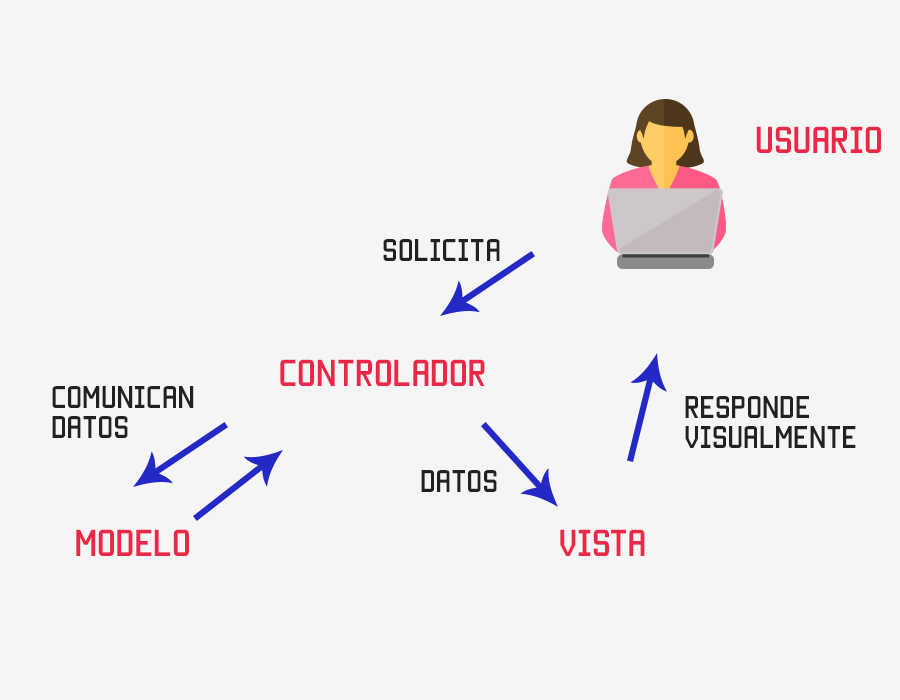
\includegraphics[scale=0.3]{mvc.jpg}}
\end{figure}

La manera en la que el usuario interactúa con el sistema será de Cliente-Servidor, lo que quiere decir que el usuario lo único que tendrá que hacer para utilizar el sistema será conectarse y acceder. Será el servidor el que tendrá todo el sistema y se encarga de responder a todas las peticiones, gestionando los dispositivos, datos y página web. 
\pagebreak

\section{Diagrama de Componentes}\label{sec:diagramaComponentes}
En esta sección se trata con más detalle cuáles serán los componentes que conforman el sistema, en forma de diagrama de componentes, que se puede ver en la \autoref{fig:diagramaComponentes}.

Esta representación permite definir de una manera estructurada y clara como se relacionan las diferentes partes del sistema, de manera que hay componentes que ofrecen interfaces a otros componentes y otros que las requieren para su correcto funcionamiento. Además, deja ver como fluye la información entre las diferentes partes del sistema y como estas la utilizan.
\begin{figure}[H]
	\ffigbox[\textwidth]
	{\caption{Diagrama de Subsistemas y Componentes}
		\label{fig:diagramaComponentes}}
	{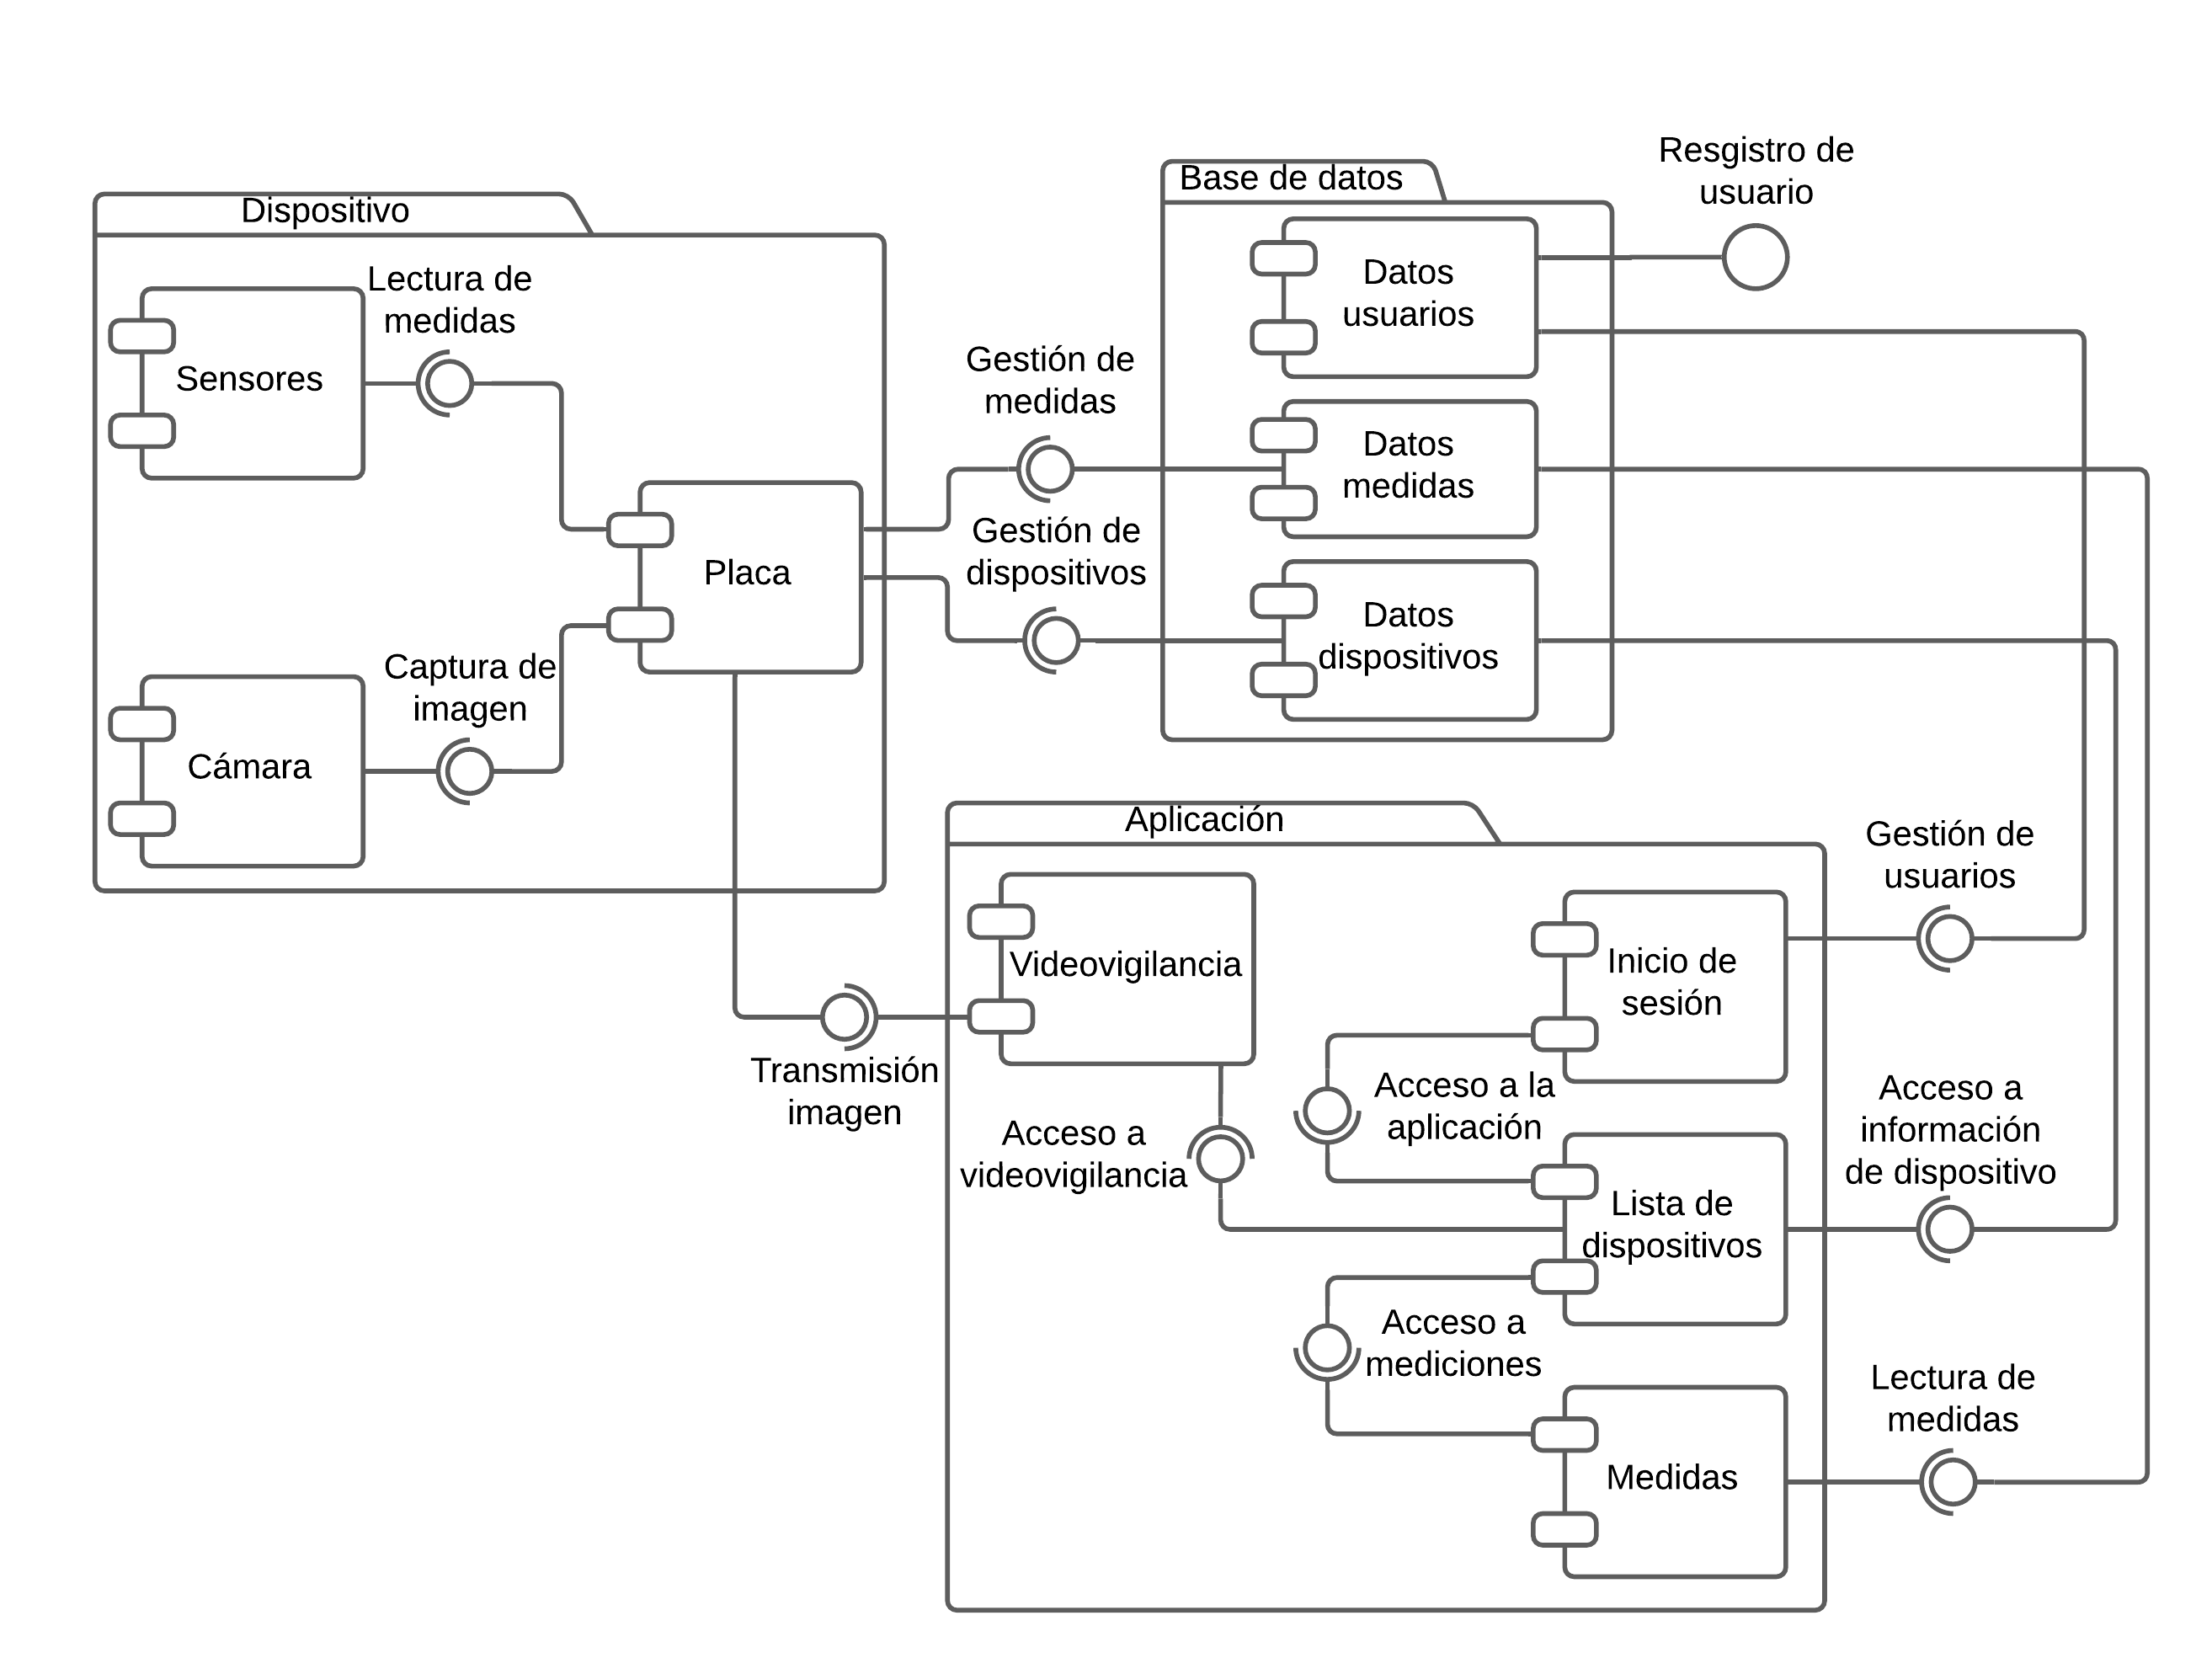
\includegraphics[width=\textwidth]{diagramaComponentes.png}}
\end{figure}
Ahora se procede a explicar los subsistemas y componentes que lo forman:
\begin{itemize}
	\item \textbf{Dispositivo:} Representa a todos los dispositivos que se encuentran conectados al sistema y que tomaran las medidas del ambiente e imagen del interior de la sala, es por esto por lo que está formado por los siguientes componentes:
	      \begin{itemize}
		      \item \textbf{Sensores:} Cada uno de los componentes conectados al dispositivo que toman medidas del ambiente. Estos están listos para ser empleados y leer las magnitudes correspondientes.
		      \item \textbf{Cámara:} Al igual que los sensores, esta será el componente conectado al dispositivo que se encargará de captar imagen del interior de la sala.
		      \item \textbf{Placa:} Componente clave del dispositivo, que dentro del mismo recogerá las lecturas de los sensores y la imagen de la sala. Una vez tiene estos datos, se encargará de enviar las mediciones a la base de datos, junto con la información de estado del propio dispositivo. Además, también transmite la imagen de la cámara vía IP para que pueda ser recogida por la aplicación.
	      \end{itemize}
	\item \textbf{Base de datos:} Representa el conjunto de tablas que conforman el modelo de datos, en el que se almacenarán las medidas, los datos del dispositivo y las credenciales de los usuarios. Sus componentes son:
	      \begin{itemize}
		      \item \textbf{Datos usuarios:} Es el componente encargado de almacenar las credenciales de usuario, que se usaran para acceder a la aplicación. Además, permite que se introduzcan nuevos usuarios mediante su registro.
		      \item \textbf{Datos medidas:} Recibe las medidas de los dispositivos mediante la interfaz gestión de medidas y responde a las solicitudes realizadas por la aplicación.
		      \item \textbf{Datos dispositivos:} Obtiene los datos de estado de los dispositivos que se encuentran en el sistema y da acceso a la aplicación a estos para ser mostrados.
	      \end{itemize}
	\item \textbf{Aplicación:} Es el subsistema con el que interactúa el usuario, al que mediante sus credenciales podrá acceder a ver los dispositivos conectados, sus mediciones y la imagen que toman. Está compuesto por:
	      \begin{itemize}
		      \item \textbf{Inicio de sesión:} Es el componente que mediante la comprobación de las credenciales de usuario, permite acceder a la aplicación y estos son verificados mediante la base de datos.
		      \item \textbf{Lista de dispositivos:} Una vez se ha iniciado sesión en la aplicación, este nos permite ver los dispositivos conectados y su estado, que se obtiene de la base de datos.
		      \item \textbf{Medidas:} Es el encargado de mostrar de manera gráfica y tabular las diferentes medidas tomadas por el dispositivo de la lista de dispositivos, estas medidas se extraen de la base de datos.
		      \item \textbf{Videovigilancia:} Es el componente encargado de mostrar la imagen en tiempo real del dispositivo instalado en la sala, recibe la imagen mediante la retransmisión del dispositivo y será accesible mediante la lista de dispositivos.
	      \end{itemize}
\end{itemize}

En las siguientes secciones se define la parte de Modelo (\autoref{sec:modelo}), Vista (\autoref{sec:interfaz}) y Controlador (\autoref{sec:servidor} y \autoref{sec:hardware}).
1\pagebreak

\section{Modelo de datos}\label{sec:modelo}
En este proyecto la base de datos es uno de los elementos más importantes que componen el sistema, no solo para permitir el acceso del personal autorizado a la aplicación, sino porque almacenará el histórico de las medidas tomadas en la sala, lo que en un futuro permitirá analizar cuál ha sido el estado de esta.

La base de datos estará alojada en el servidor, donde la aplicación podrá acceder a ella más fácilmente para su visualización y consulta, además, facilita que se puedan centralizar las medidas en un único lugar, para el caso en el que se tuvieran múltiples dispositivos en un edificio y se deseara consultarlos desde un mismo lugar.

Como se comentó en la \autoref{subsec:servidorDB} se utiliza una base de datos MariaDB, que se administra mediante phpMyAdmin \cite{noauthor_phpmyadmin_nodate}, que es un administrador de base de datos para realizar la mayoría de las tareas de una manera más sencilla y eficiente.

\subsection{Estructura de tablas de la base de datos}
Se presentan en esta subsección las tablas que componen la base de datos, indicando la utilidad de cada una de ellas y los datos, con sus tipos, que se almacenan en ellas. Antes de pasar a explicarlas en más detalle en la \autoref{fig:distDB} se puede ver un resumen de estas.
\begin{figure}[H]
	\ffigbox[\FBwidth]
	{\caption{Distribución de tablas en la base de datos}
		\label{fig:distDB}}
	{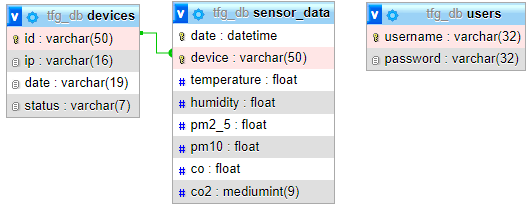
\includegraphics[scale=0.85]{db_dist.png}}
\end{figure}
\subsubsection{Tabla de usuarios}
En esta tabla se almacenan las credenciales de los usuarios que utilicen la aplicación. Estas credenciales se consultan cuando un usuario trata de iniciar sesión y serán añadidas por el administrador del sistema en esta tabla. Es importante destacar que la contraseña se almacena en formato hash (encriptada) para evitar que se pueda leer si llega a haber alguna intrusión. 
\pagebreak

A continuación, en la \autoref{tab:tabla_users} se muestra la estructura de la tabla:
\begin{table}[H]
	\centering
	\caption{Tabla users BBDD}
	\label{tab:tabla_users}
	\resizebox{\textwidth}{!}{%
		\begin{tabular}{|p{.2\textwidth}|p{.2\textwidth}|p{.6\textwidth}|}
			\hline
			\rowcolor[HTML]{BFBFBF}
			\multicolumn{1}{|c|}{\cellcolor[HTML]{BFBFBF}{\color[HTML]{000000} \textbf{Nombre}}} & \multicolumn{1}{c|}{\cellcolor[HTML]{BFBFBF}{\color[HTML]{000000} \textbf{Tipo}}} & \multicolumn{1}{c|}{\cellcolor[HTML]{BFBFBF}{\color[HTML]{000000} \textbf{Descripción}}} \\ \hline
			username                                                                             & varchar(32)                                                                       & Nombre de usuario que identifica unívocamente al usuario                                 \\ \hline
			password                                                                             & varchar(32)                                                                       & MD5 de la clave de acceso que debe proporcionar para verificar su identidad              \\ \hline
		\end{tabular}%
	}
\end{table}
La clave primaria será el username, de esta manera no habrá ningún problema de duplicidad de usuarios en la base de datos.

\subsubsection{Tabla de dispositivos}
En esta tabla se registran los dispositivos que se han conectado con el servidor, estos dispositivos son los que se pueden consultar desde la aplicación y que se muestran con la fecha de actualización junto con su estado actual.

En la \autoref{tab:tabla_devices} se pueden ver los atributos que la componen:

\begin{table}[H]
	\centering
	\caption{Tabla devices BBDD}
	\label{tab:tabla_devices}
	\resizebox{\textwidth}{!}{%
		\begin{tabular}{|p{.2\textwidth}|p{.2\textwidth}|p{.6\textwidth}|}
			\hline
			\rowcolor[HTML]{BFBFBF}
			\multicolumn{1}{|c|}{\cellcolor[HTML]{BFBFBF}{\color[HTML]{000000} \textbf{Nombre}}} & \multicolumn{1}{c|}{\cellcolor[HTML]{BFBFBF}{\color[HTML]{000000} \textbf{Tipo}}} & \multicolumn{1}{c|}{\cellcolor[HTML]{BFBFBF}{\color[HTML]{000000} \textbf{Descripción}}} \\ \hline
			id                                                                                   & varchar(50)                                                                       & Nombre identificativo del dispositivo, su dirección física                               \\ \hline
			ip                                                                                   & varchar(16)                                                                       & IP de la red local desde la que se puede acceder a sus datos                             \\ \hline
			date                                                                                 & datetime                                                                          & Fecha de la última actualización de estado                                               \\ \hline
			status                                                                               & varchar(7)                                                                        & Estado del dispositivo, Online u Offline                                                 \\ \hline
		\end{tabular}%
	}
\end{table}
Como en la \autoref{tab:tabla_users} la clave primaria de esta es un nombre representativo, en este caso el id, que identifica inequívocamente al dispositivo, de esta manera se puede utilizar para consultar los datos de un dispositivo en concreto. Cuando sea necesario, se puede variar la IP a la que está conectado, la fecha y el estado, pero el nombre identificador no se puede cambiar.

\subsubsection{Tabla de medidas}
Es la tabla más importante como ya se ha mencionado. En esta tabla se guardan las mediciones que han tomado todos los dispositivos conectados. Estos datos son los que se muestran en la página del dispositivo dentro de la aplicación, junto con su imagen en tiempo real. Las medidas que se almacenan son: temperatura, humedad, PM$_{2.5}$, PM$_{10}$, CO y CO$_2$.

Los datos que la componen se exponen en la \autoref{tab:tabla_sensor_data}:

\begin{table}[H]
	\centering
	\caption{Tabla sensor\_data BBDD}
	\label{tab:tabla_sensor_data}
	\resizebox{\textwidth}{!}{%
		\begin{tabular}{|p{.2\textwidth}|p{.2\textwidth}|p{.6\textwidth}|}
			\hline
			\rowcolor[HTML]{BFBFBF}
			\multicolumn{1}{|c|}{\cellcolor[HTML]{BFBFBF}{\color[HTML]{000000} \textbf{Nombre}}} & \multicolumn{1}{c|}{\cellcolor[HTML]{BFBFBF}{\color[HTML]{000000} \textbf{Tipo}}} & \multicolumn{1}{c|}{\cellcolor[HTML]{BFBFBF}{\color[HTML]{000000} \textbf{Descripción}}} \\ \hline
			date                                                                                 & datetime                                                                          & Fecha en la que se ha tomado la medida                                                   \\ \hline
			device                                                                               & varchar(50)                                                                       & Identificador del dispositivo que captó la medida                                        \\ \hline
			temperature                                                                          & float                                                                             & Temperatura de la sala                                                                   \\ \hline
			humidity                                                                             & float                                                                             & Humedad de la sala                                                                       \\ \hline
			pm2\_5                                                                               & float                                                                             & Cantidad de partículas de 2.5 $\mu m$ en la sala                                         \\ \hline
			pm10                                                                                 & float                                                                             & Cantidad de partículas de 10 $\mu m$ en la sala                                          \\ \hline
			co                                                                                   & float                                                                             & Porcentaje de CO en el aire de la sala                                                   \\ \hline
			co2                                                                                  & mediumint(9)                                                                      & Partículas por millón de CO$_2$ en la sala                                               \\ \hline
		\end{tabular}%
	}
\end{table}
Las claves primarias son date y device, estas claves identifican de manera única a cada una de las medidas, por lo que se puede consultar una medida concreta de un dispositivo específico.

Además, existe una relación directa con la tabla devices en cuanto a que el campo device es una clave ajena del campo id, de esta manera cuando un dispositivo sea eliminado o actualizado se propaga a esta tabla.

\section{Interfaz de Usuario}\label{sec:interfaz}
En esta sección se trata otro de los elementos clave del sistema, la interfaz de usuario. Esta hace posible el uso del sistema a personas no expertas, de manera que puedan manipularlo y hacer uso de este sin la necesidad de saber cómo se desarrolla un sistema de estas características.

La parte del sistema a la que se ha dotado de interfaz es la responsable de mostrar las medidas y video de las salas, tal y como ha solicitado el cliente. Para lograr esto se utiliza una página web, que se ha diseñado en HTML y CSS, con la que se puede acceder a toda esta información de una manera sencilla y visual. En cuanto a la lógica para obtener la información y movernos por las pantallas se emplea PHP.

La web, además, es \textit{responsive} por lo que es totalmente funcional tanto en dispositivos de altas resoluciones (televisiones, ordenadores de sobremesa, portátiles, etc.), como en dispositivos de bajas resoluciones (móviles, tablets, etc.).

En la \autoref{fig:flujo_interfaz} se muestra el flujo de pantallas e interacciones que se sigue al acceder a la aplicación web, más tarde se explica en detalle cada una de las pantallas de la interfaz y que interacciones nos permite.
\begin{figure}[H]
	\ffigbox[\FBwidth]
	{\caption{Diagrama de flujo de la web}
		\label{fig:flujo_interfaz}}
	{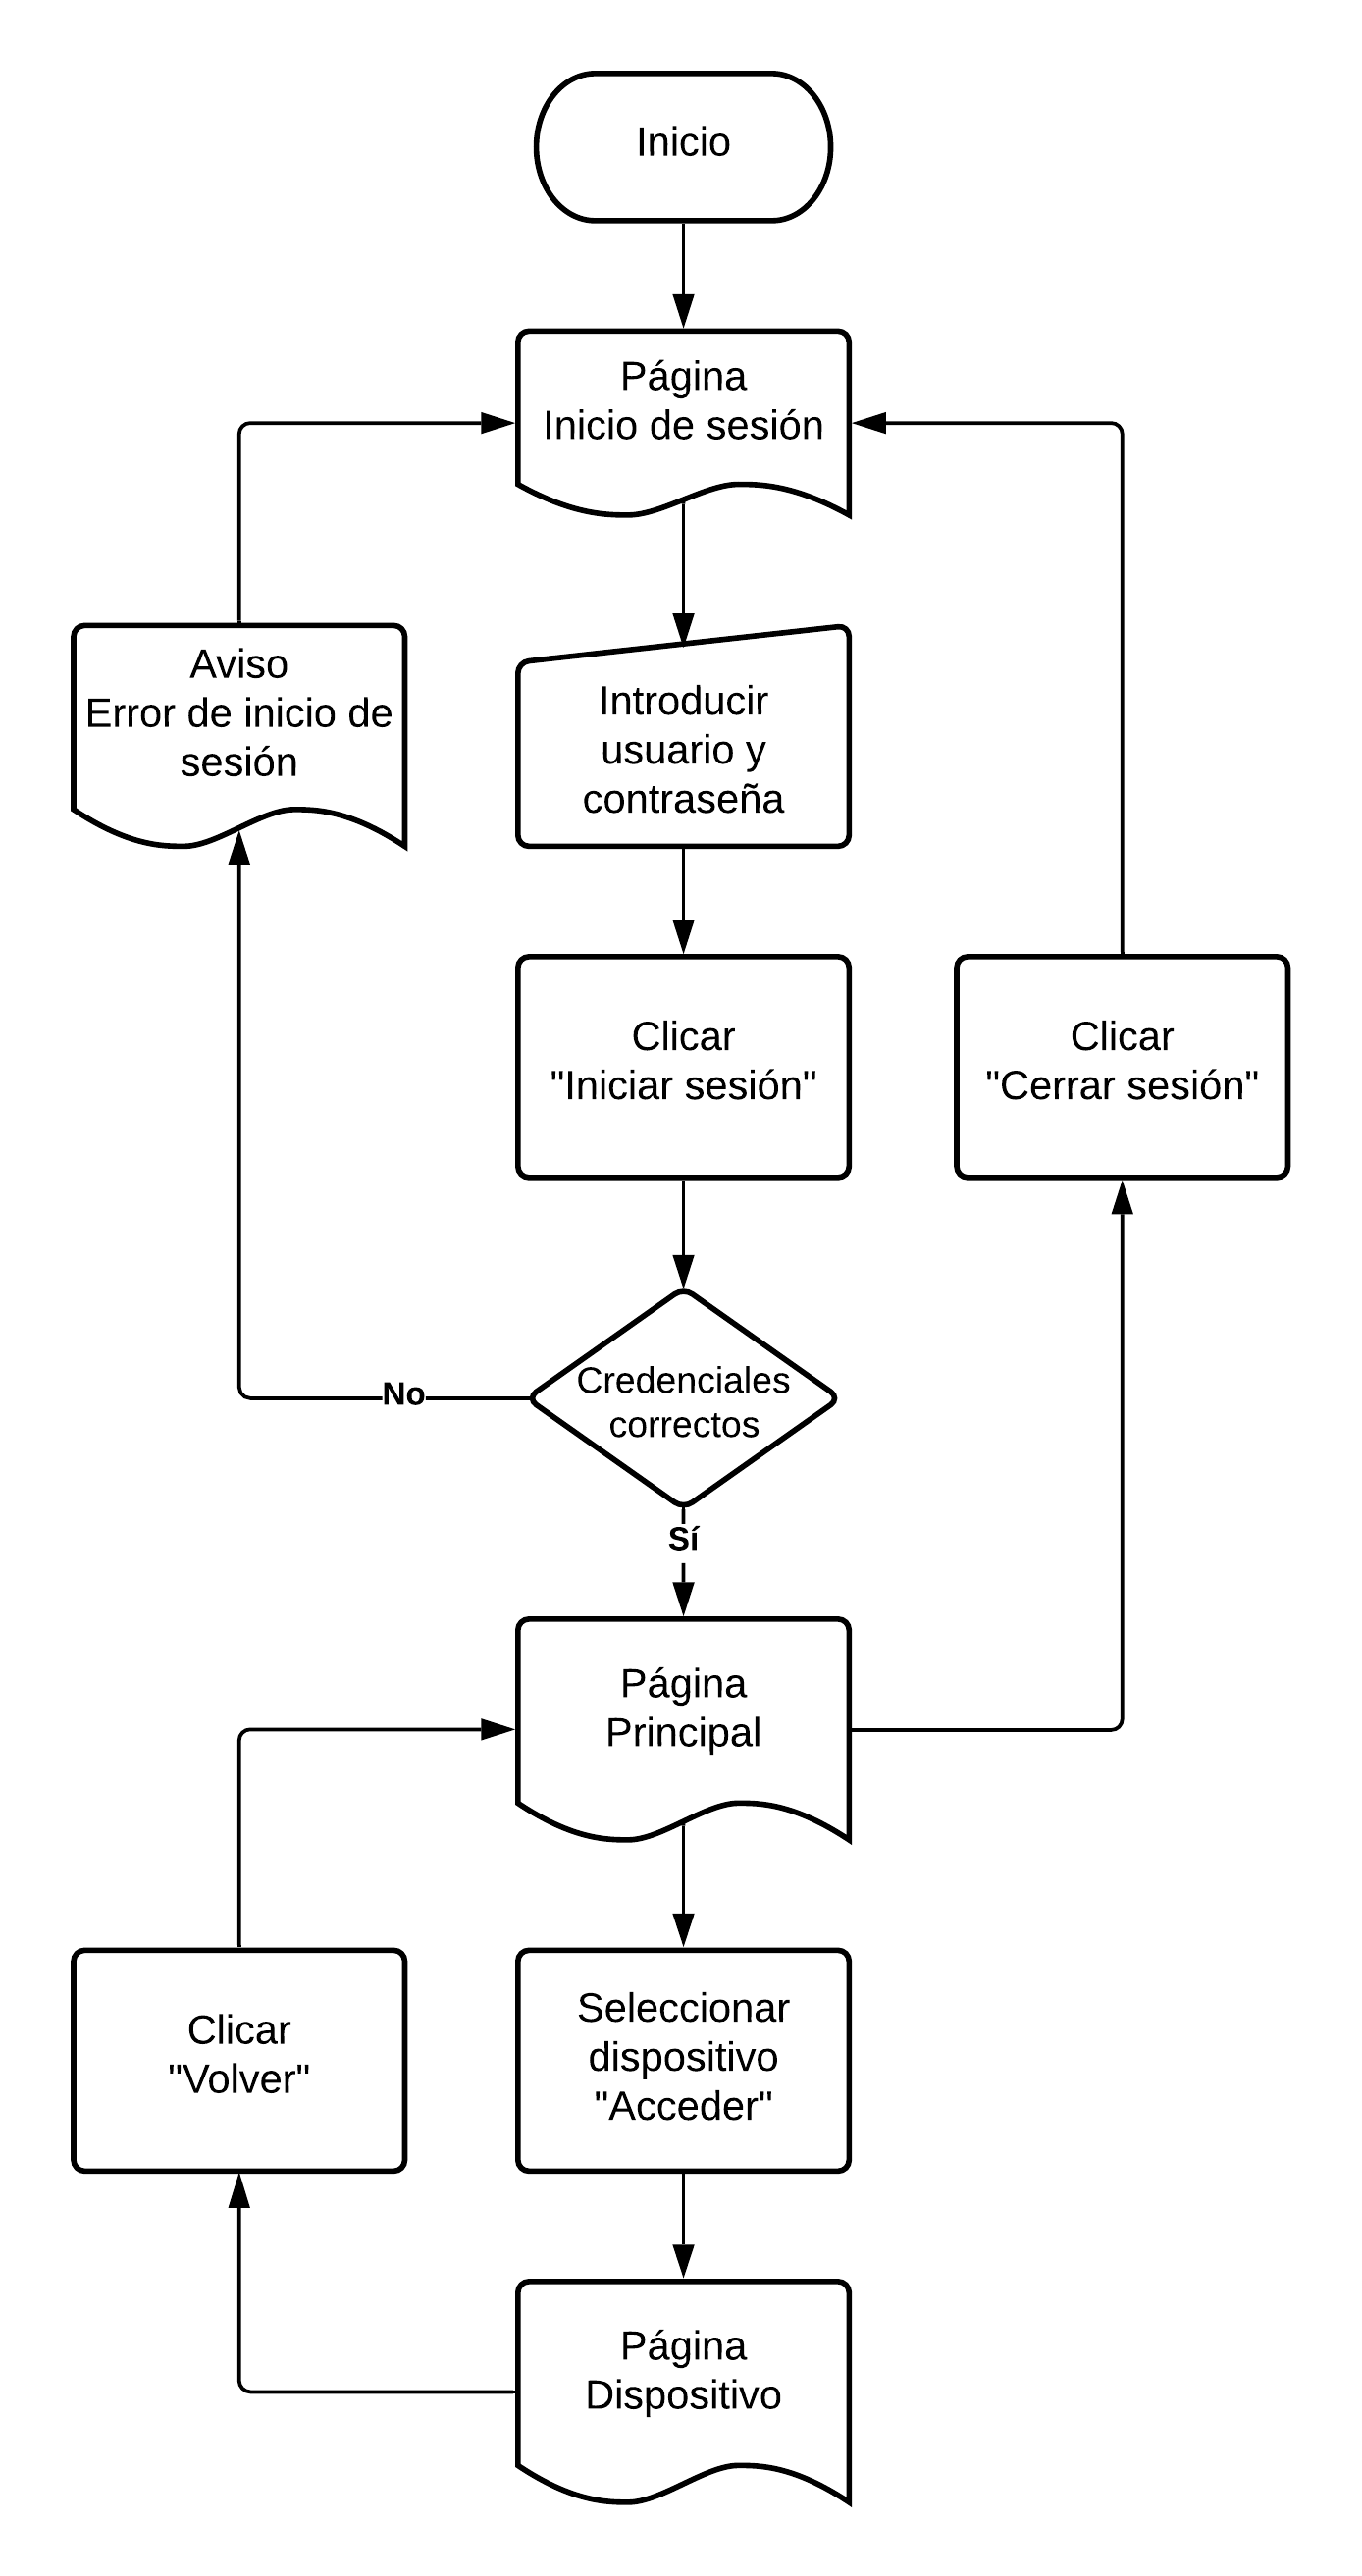
\includegraphics[scale=1]{flujoInterfaz.png}}
\end{figure}

\subsection{Página: Inicio de sesión}\label{subsec:iLogin}
Es la primera pantalla que se encontrara el usuario cuando acceda a la aplicación, en esta, como se puede ver en la \autoref{fig:iLogin} se le solicita introducir su nombre de usuario y contraseña de acceso. Esta pantalla es fundamental para garantizar la seguridad del centro, de manera que no accedan personas no autorizadas y que puedan poner en riesgo su seguridad.
\begin{figure}[H]
	\ffigbox[\textwidth]
	{\caption{Interfaz de inicio de sesión}
		\label{fig:iLogin}}
	{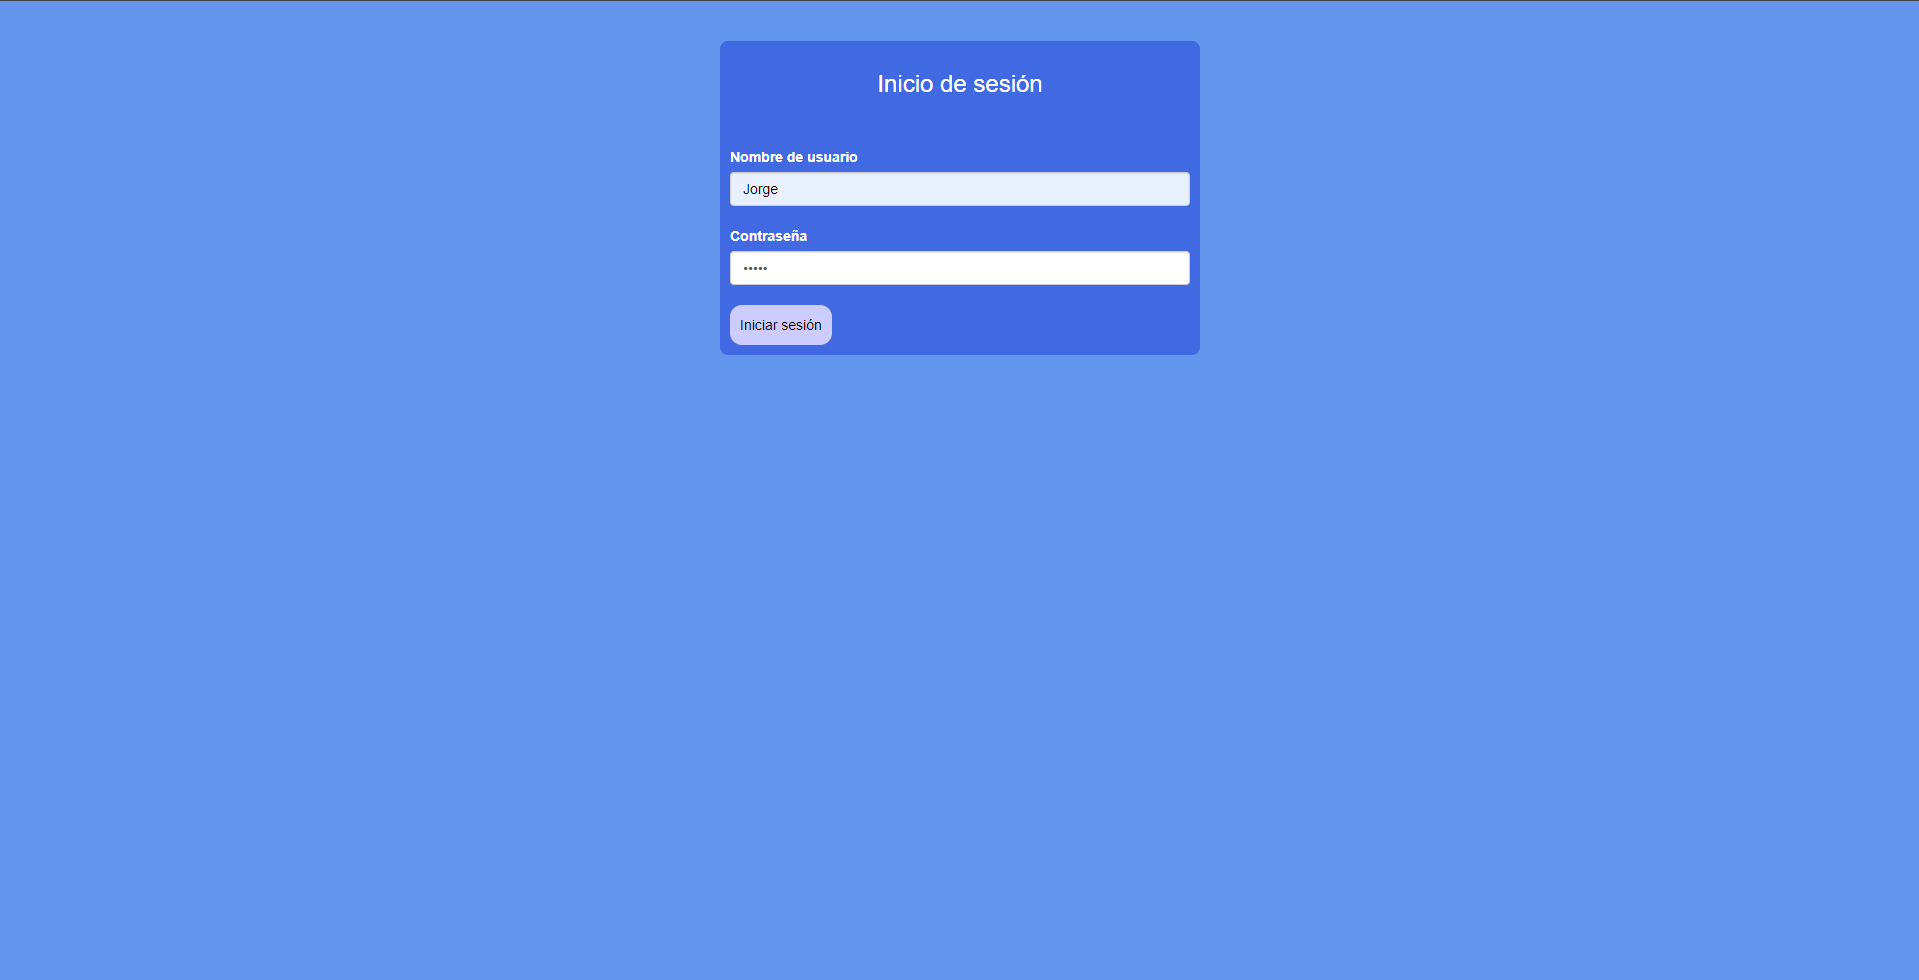
\includegraphics[width=\textwidth]{login.png}}
\end{figure}
Como se puede observar, la paleta de colores se adapta a lo solicitado por el cliente, utilizando colores de la gama de los azules que contrasten entre ellos, de manera que se puedan visualizar sin dificultad todos los elementos de esta. Los códigos RGB hexadecimales elegidos son:
\begin{itemize}
	\item Primario: \#4169e1
	\item Secundario: \#4169e1
	\item Primario claro: \#191970
	\item Secundario Oscuro: \#ccccff
	\item Resaltado: \#9e9eff
	\item Gris: \#dddddd
\end{itemize}
En el primer campo, correspondiente al nombre de usuario, se muestra el texto escrito, sin embargo, en el de la contraseña los caracteres del texto se sustituirán visualmente por asteriscos, garantizando la privacidad de la contraseña.

En el caso de introducir unas credenciales no registradas en el sistema se avisa al usuario de que revise lo que ha escrito, ''Compruebe las credenciales'', dado que si no coinciden no se puede garantizar su identidad.

Por otro lado, también se deben completar ambos campos, si esto no es así se lanza un aviso al usuario informándole de que los debe cumplimentar si desea acceder, ''Ambos campos son obligatorios''.

Una vez el usuario ha completado los campos podrá hacer clic en el botón ''Iniciar sesión'' y si cumple todo lo anterior le llevará a la pantalla principal descrita en la \autoref{subsec:iPrincipal}.

En cuanto a la versión móvil, se ha ajustado el tamaño del formulario para que se adapte y sea legible incluso en resoluciones pequeñas. Además, el tamaño de letra es suficientemente grande, 14 pixeles para formulario y 10 pixeles para el botón, como para que se pueda leer correctamente tanto en grandes como en pequeñas resoluciones.
\begin{figure}[H]
	\ffigbox[\FBwidth]
	{\caption{Interfaz de inicio de sesión en móvil}
		\label{fig:iLoginM}}
	{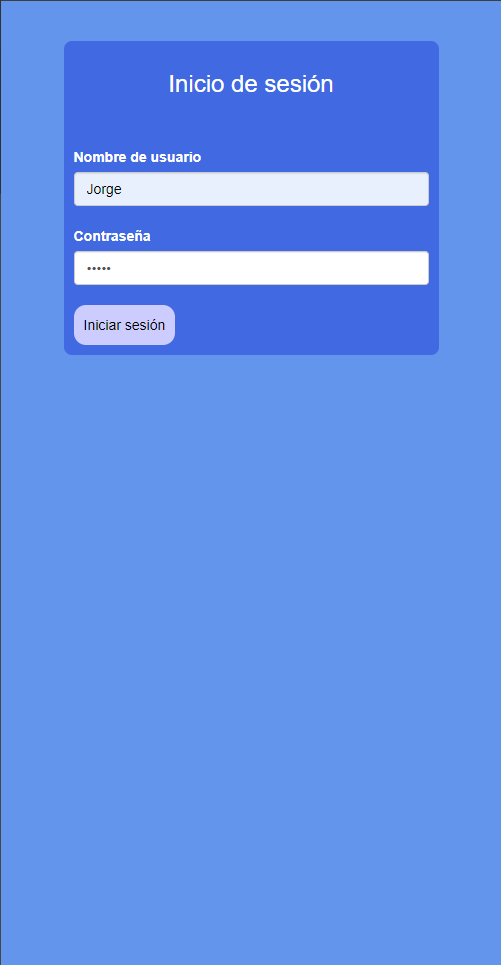
\includegraphics[scale=0.55]{loginM.png}}
\end{figure}

\subsection{Página: Principal}\label{subsec:iPrincipal}
Una vez el usuario ha iniciado la sesión de manera satisfactoria, se pasará a la pantalla mostrada en la \autoref{fig:iPrincipal}, en la que se puede ver que muestra un mensaje de saludo, indicando el nombre de usuario.

La clave de esta pantalla es la lista de los dispositivos, en la que se muestran de manera tabular los datos de estos. Se imprime, para cada dispositivo, los datos almacenados en la base.
\vspace{.5cm}
\begin{figure}[H]
	\ffigbox[\textwidth]
	{\caption{Interfaz de pantalla principal}
		\label{fig:iPrincipal}}
	{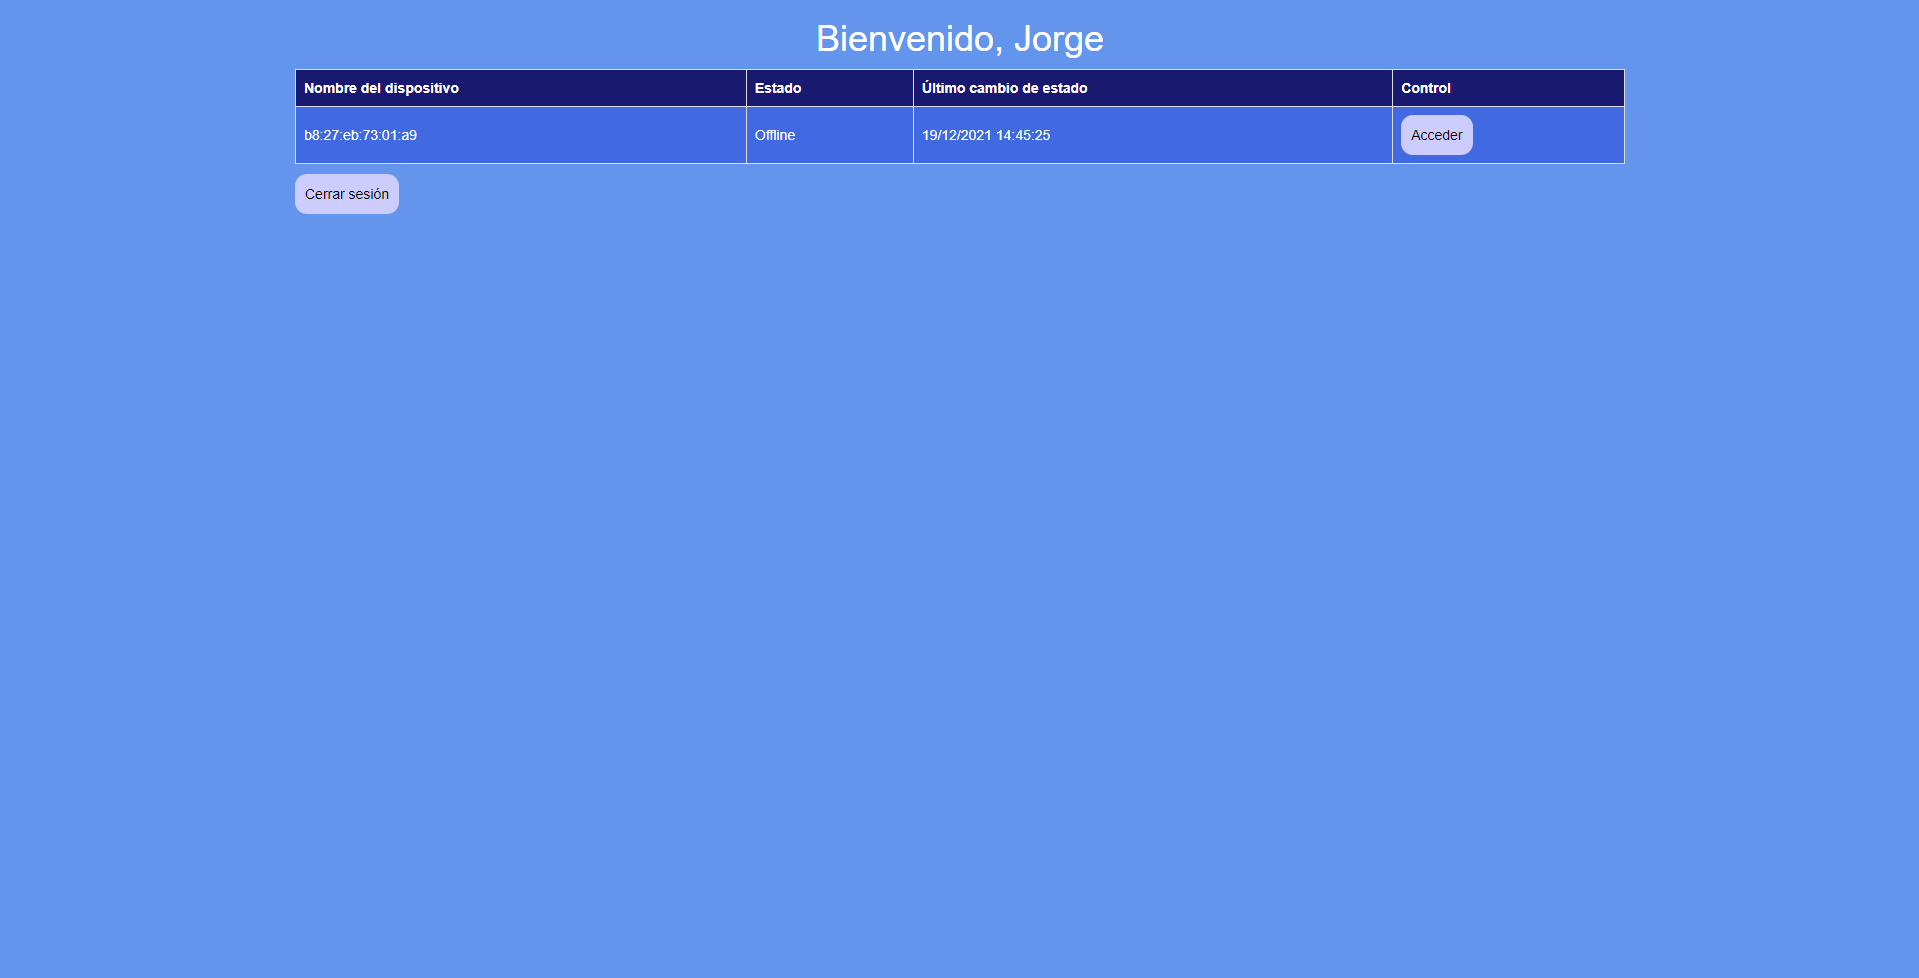
\includegraphics[width=\textwidth]{devices.png}}
\end{figure}
En la última posición de cada fila de dispositivos hay un botón en el que pone ''Acceso'' que nos redirige a la página de dispositivo, que se describe en la \autoref{subsec:iDispositivo}.

En la parte inferior aparece un botón con el texto ''Cerrar sesión'' que como su propio nombre indica, cierra la sesión y nos devuelve a la página de inicio de sesión, \autoref{subsec:iLogin}.

Por último, en la versión móvil la tabla pasará a ocupar el ancho completo de la pantalla para que se pueda ver claramente el botón de la última posición y facilitar acceder al dispositivo. En cuanto al texto de saludo, se ha decidido mantenerlo, pero ajustándose para que no se salga de la pantalla, evitando el \textit{scroll} lateral.
\vspace{.5cm}
\begin{figure}[H]
	\ffigbox[\FBwidth]
	{\caption{Interfaz de pantalla principal en móvil}
		\label{fig:iPrincipalM}}
	{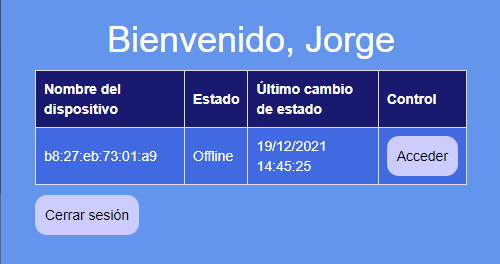
\includegraphics[scale=0.6]{devicesM.png}}
\end{figure}

\subsection{Página: Dispositivo}\label{subsec:iDispositivo}
Esta pantalla muestra la información clave de este proyecto, la imagen de la cámara del dispositivo y las medidas tomadas. 

A esta pantalla se accede una vez se ha seleccionado un dispositivo en la página principal, \autoref{subsec:iPrincipal}, y tiene la apariencia que se muestra en la \autoref{fig:iDispositivoI}, \autoref{fig:iDispositivoII} y \autoref{fig:iDispositivoIII}.

En primer lugar, en la parte superior se muestra el nombre que identifica al dispositivo, de manera que podemos saber, en todo momento, que datos estamos consultando.

Inmediatamente después, se muestra un cuadro con la imagen en tiempo real de la cámara del dispositivo.
\begin{figure}[H]
	\ffigbox[\textwidth]
	{\caption{Interfaz de dispositivo I}
		\label{fig:iDispositivoI}}
	{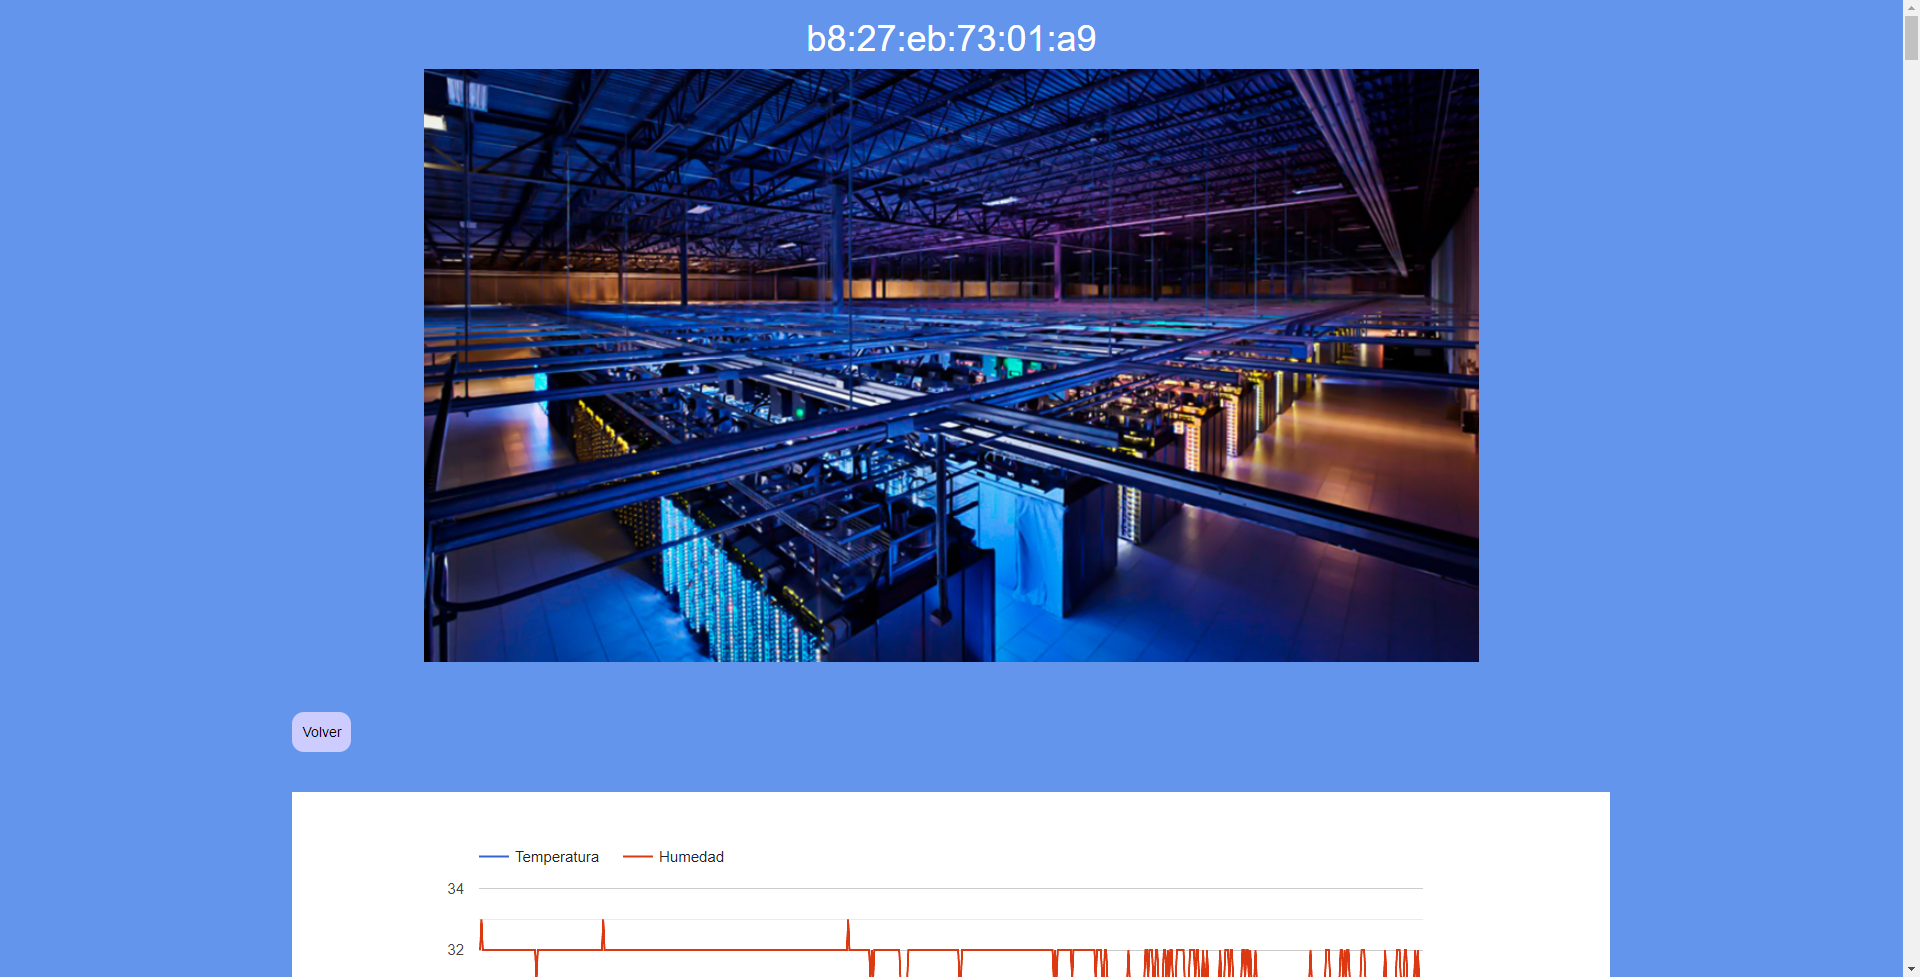
\includegraphics[width=\textwidth]{medidas1.png}}
\end{figure}
A continuación, se mostrarán todas las medidas, primero de manera gráfica y después de manera tabular.

La parte visual de las medidas se divide en 3 gráficas distintas, para poder ver mejor como progresan en el tiempo sin que haya problemas de escalas entre ellas y sin saturar la pantalla. Las gráficas son:
\begin{itemize}
	\item Temperatura y Humedad.
	\item PM$_{2.5}$, PM$_{10}$ y CO.
	\item CO$_2$.
\end{itemize}
\begin{figure}[H]
	\ffigbox[\textwidth]
	{\caption{Interfaz de dispositivo II}
		\label{fig:iDispositivoII}}
	{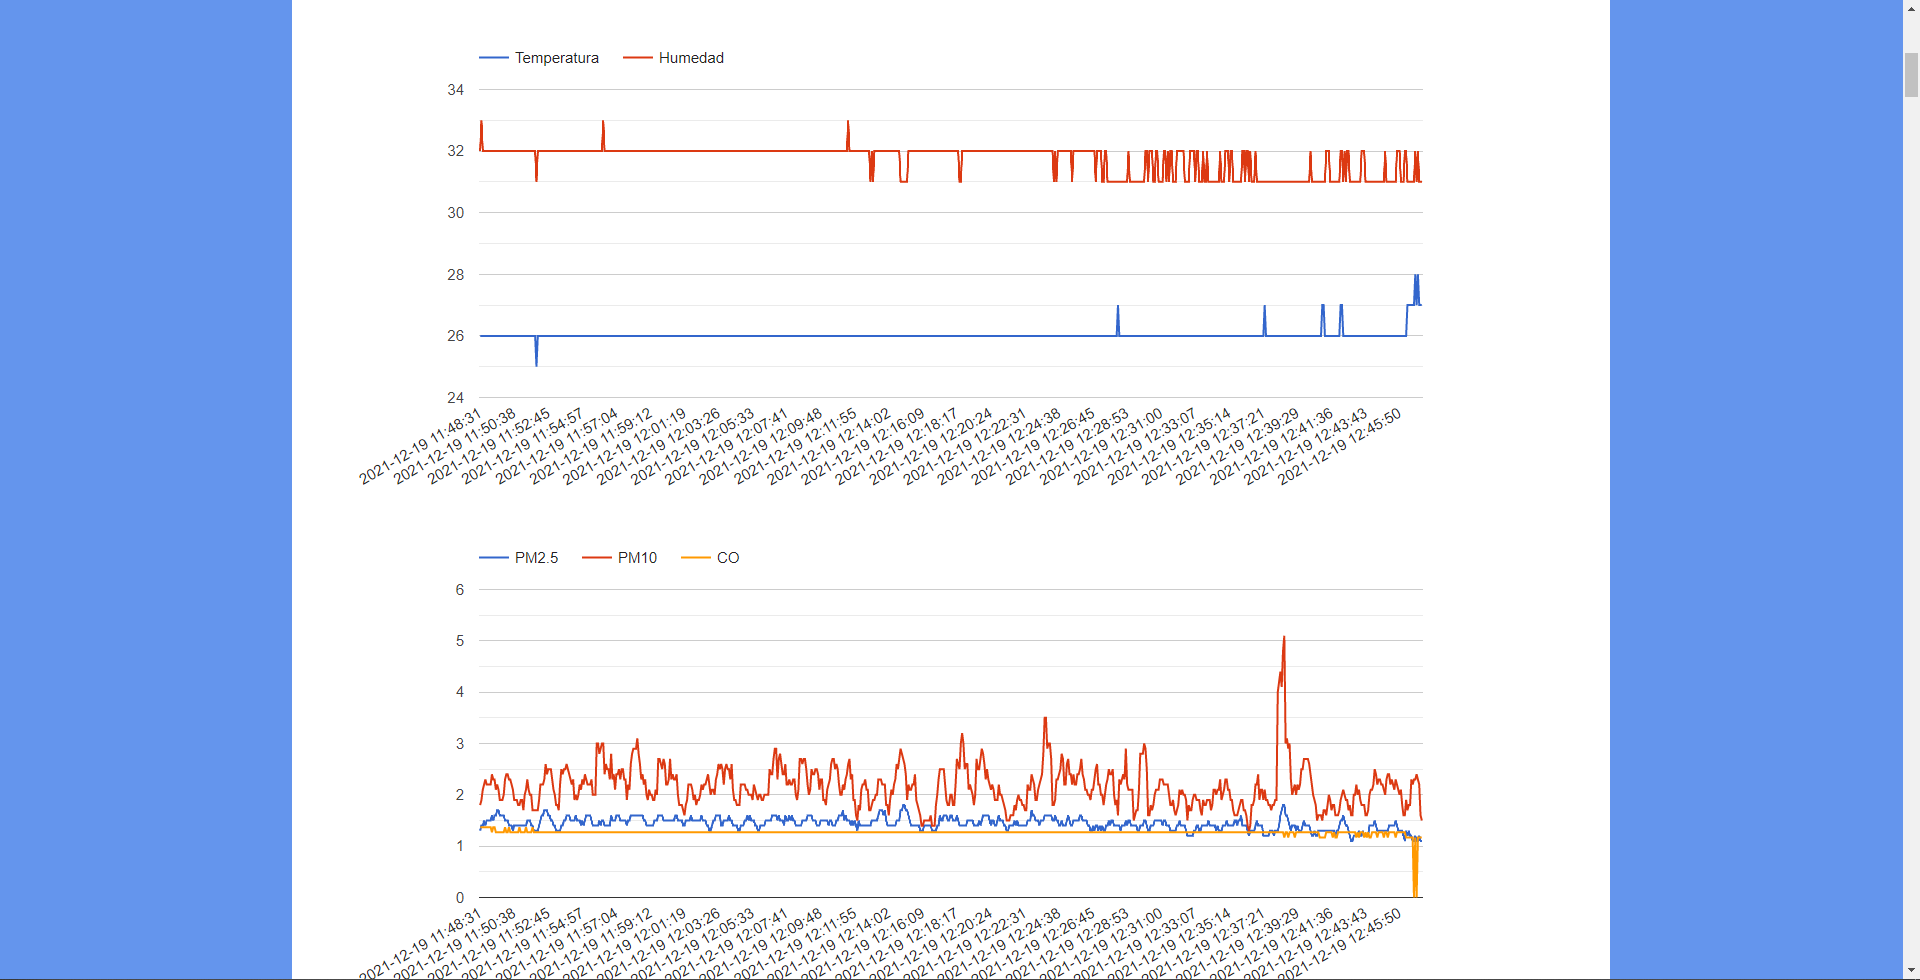
\includegraphics[width=\textwidth]{medidas2.png}}
\end{figure}
En cuanto a la forma tabular, mediante una tabla se muestran las medidas de manera cronológica, de más reciente a más antigua. Esta tabla está compuesta por los 720 últimos registros, que cubren la última hora de mediciones de la sala, puesto que se toma una medida cada 5 segundos.
\vspace{.5cm}
\begin{figure}[H]
	\ffigbox[\textwidth]
	{\caption{Interfaz de dispositivo III}
		\label{fig:iDispositivoIII}}
	{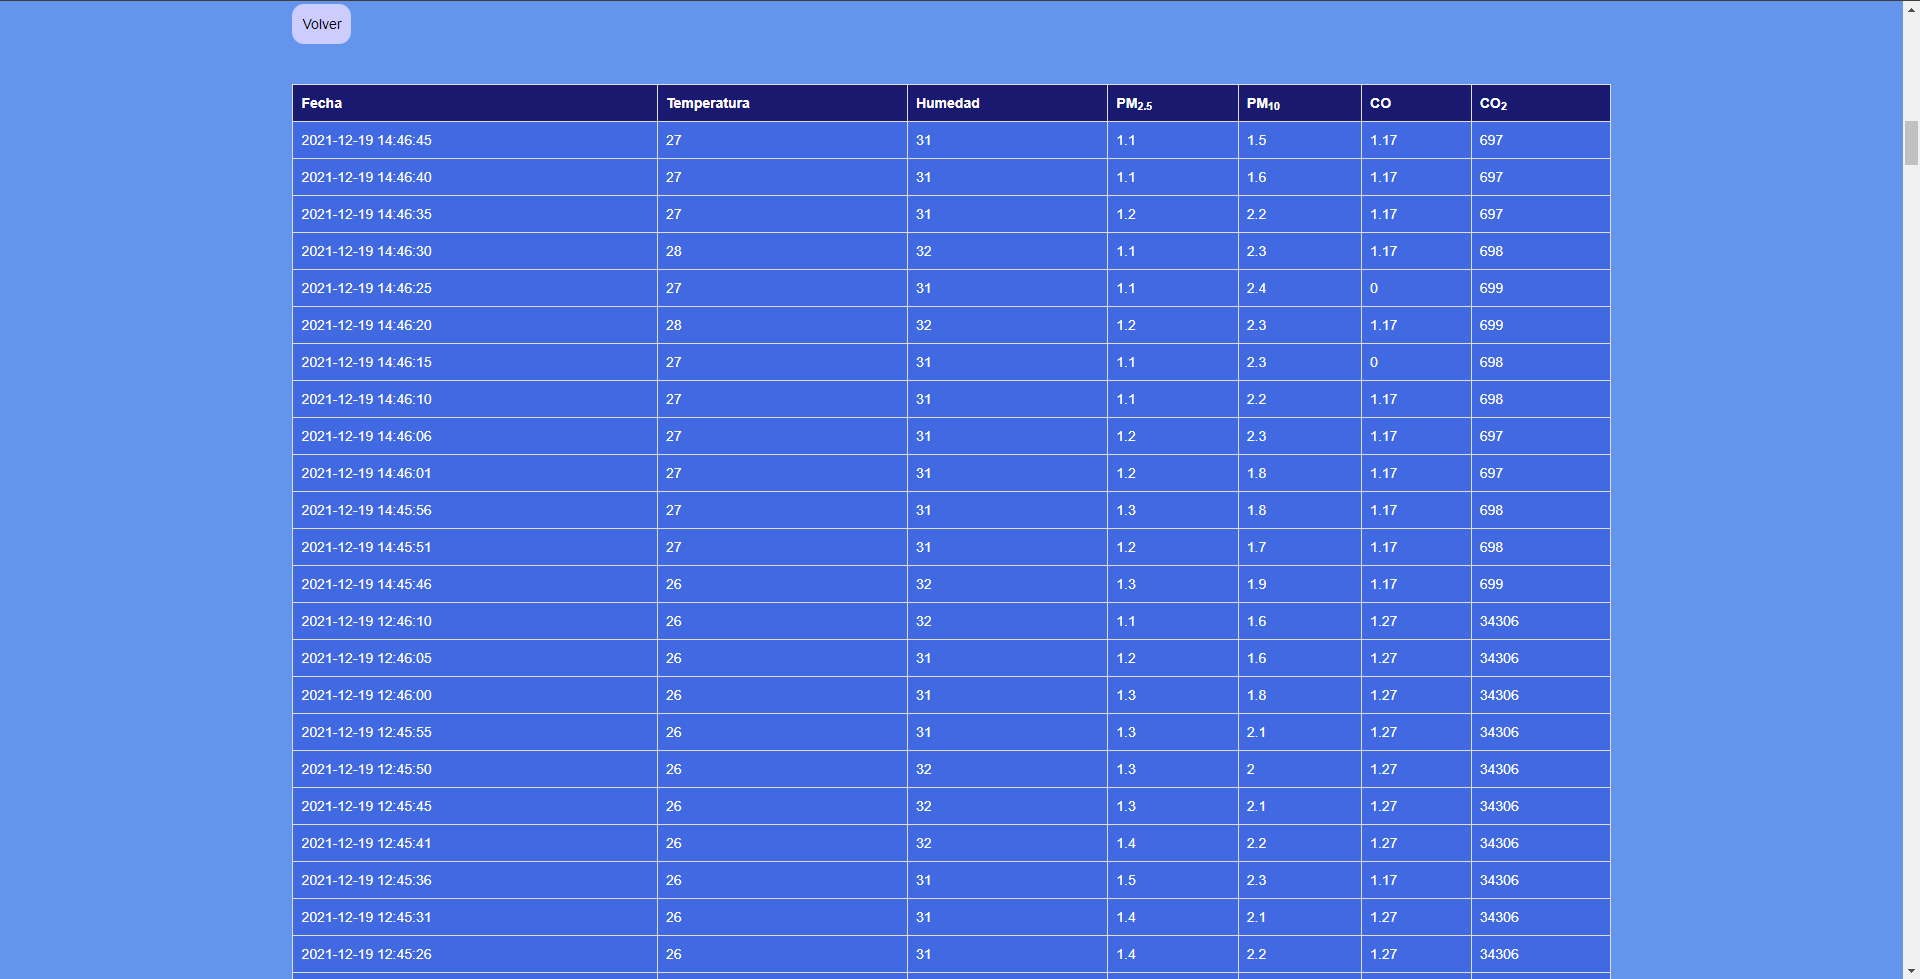
\includegraphics[width=\textwidth]{medidas3.png}}
\end{figure}

Para la versión móvil se ajusta el tamaño de la cámara, gráficas y tabla al ancho del dispositivo, de manera que se puedan visualizar bien todos los datos, evitando así tener que hacer zum en la pantalla.
\pagebreak

Además, las gráficas ofrecen la posibilidad de acceder a un dato en particular si hacemos clic o tocamos una sección específica, indicando los valores y momento específicos.
\begin{figure}[H]
	\ffigbox[\FBwidth]
	{\caption{Interfaz de dispositivo en móvil}
		\label{fig:iDispositivoMI}}
	{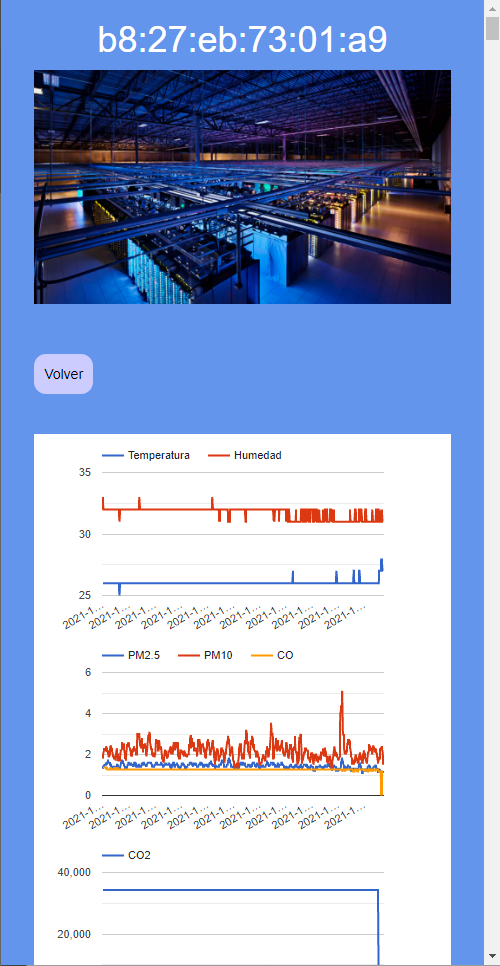
\includegraphics[scale=0.5]{medidas1M.png}
		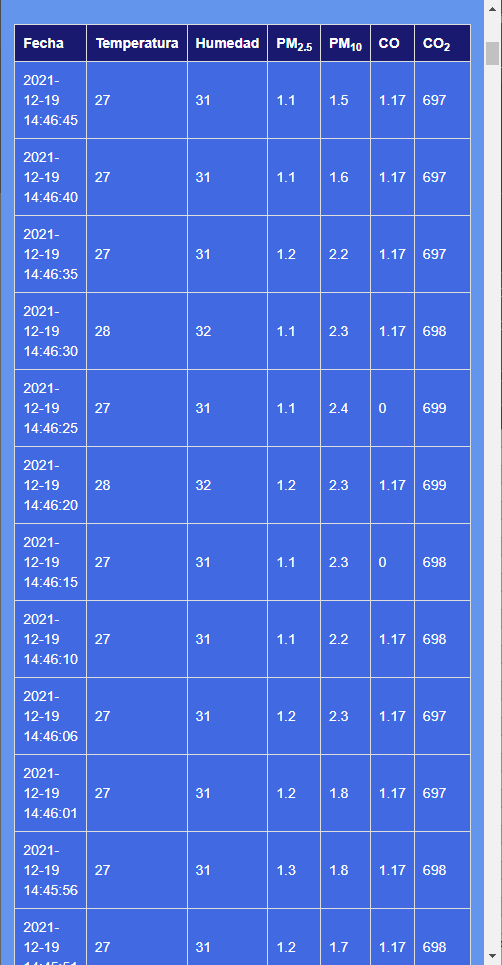
\includegraphics[scale=0.5]{medidas3M.png}}
\end{figure}

\section{Servidor}\label{sec:servidor}
Como ya se especifica en la \autoref{subsec:servidorDB}, el servidor que se emplea para alojar la página web es Apache, que cubre todas las necesidades de la aplicación, dado que nos permite lanzar al público un sitio web desarrollado en el lenguaje PHP. Este lenguaje de desarrollo web nos facilita la implementación de la lógica y acceso a la base de datos, a la vez que diseñar las pantallas vistas en la \autoref{sec:interfaz}. 

En el mismo servidor se aloja la base de datos tal y como ha quedado descrita en la \autoref{sec:modelo}, eso permite que sea accesible para el dispositivo de medición y videovigilancia, que posee los permisos para acceder a la misma.
\pagebreak

\section{Hardware}\label{sec:hardware}
En cuanto a la parte física del proyecto, se detalla en esta sección cuáles son las conexiones entre los diferentes elementos que se describieron en la \autoref{sec:hardwareSoftware} y que son los elegidos para formar parte de este. La conexión se resume en el esquema de la \autoref{fig:circuito}. Este esquema se ha realizado con Fritzing \cite{noauthor_fritzing_nodate} que nos permite de una manera sencilla importar y conectar los componentes.
\begin{figure}[H]
	\ffigbox[\textwidth]
	{\caption{Esquema de conexiones dispositivo}
		\label{fig:circuito}}
	{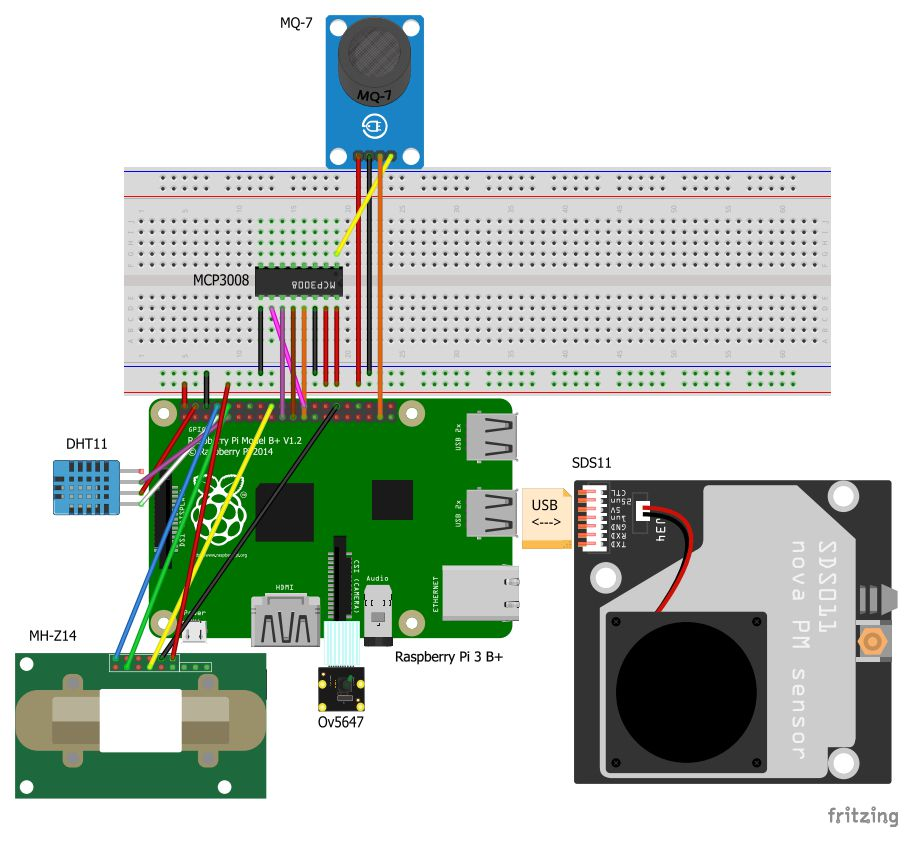
\includegraphics[width=\textwidth]{circuito.jpg}}
\end{figure}

Se comienza con los sensores con los que cuenta el dispositivo:
\begin{itemize}
	\item \textbf{DHT11}: Se trata del sensor de temperatura y humedad elegido.
	      
	      Por medio de la conexión de DATA con GPIO 4, indicada con el cable blanco, se obtiene la temperatura y la humedad del ambiente. 
	      
	      El cable rojo lo conecta con la corriente de 5 V.
	      
	      El cable morado lo conecta a un puerto de tierra, GND.
	\item \textbf{MQ-7}: Es el sensor de dióxido de carbono. Al tratarse de un sensor analógico y dado que la Raspberry no posee pines de este tipo se emplea un conversor MCP3008 que nos proporciona 8 canales analógicos de 10 bits.
	      
	      Se conecta mediante la protoboard a la corriente de 5 V y a tierra, cable rojo y negro respectivamente.
	      
	      En cuanto a los datos se conecta al conversor con el cable amarillo y al GPIO 26 mediante el naranja.
	      
	      El conversor se conecta a la corriente y a tierra mediante la protoboard, como el sensor, pero este además se debe conectar a los puertos SPIO\_MOSI, SPIO\_MISO, SPIO\_SCLK y SPIO\_CE0 para ofrecer los puertos analógicos. El conversor sigue el esquema de la \autoref{fig:MCP3008} \cite{noauthor_27v_2008} y para su uso se consulta la guía \cite{noauthor_raspberry_nodate-1}.
	      \begin{figure}[H]
		      \ffigbox[\FBwidth]
		      {\caption{Esquema conversor MCP3008}
			      \label{fig:MCP3008}}
		      {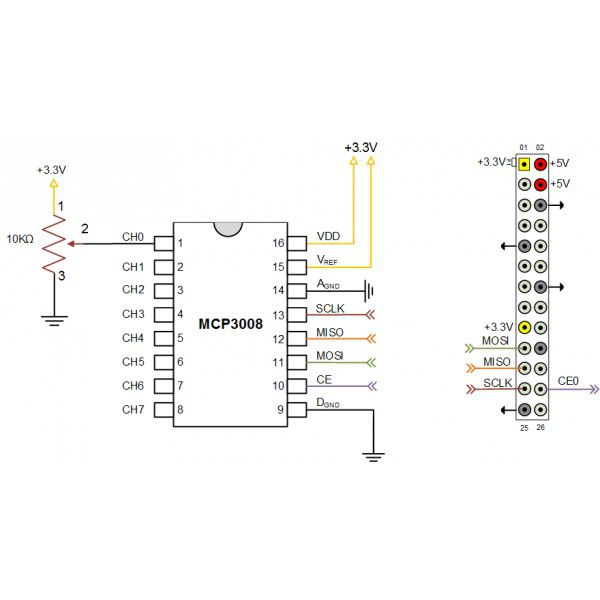
\includegraphics[scale=0.5]{mcp3008.jpg}}
	      \end{figure}
	\item \textbf{MH-Z14}: Es el sensor de CO$_2$ empleado.
	      
	      Se alimenta mediante el cable rojo a la corriente de 5 V y a tierra mediante el cable negro, ambos por medio de la protoboard. Se emplea la protoboard por falta de puertos únicos de corriente.
	      
	      Por otro lado, para transmitir los datos de las medidas utiliza los cables azul y verde a los puertos UART\_TXD y UART\_RXD respectivamente. Además, con el cable amarillo se une la salida analógica con el GPIO 24. El esquema de los pines se puede ver en la \autoref{fig:MH-Z14} \cite{noauthor_documentacion_nodate}.
	      \begin{figure}[H]
		      \ffigbox[\FBwidth]
		      {\caption{Esquema del sensor MH-Z14}
			      \label{fig:MH-Z14}}
		      {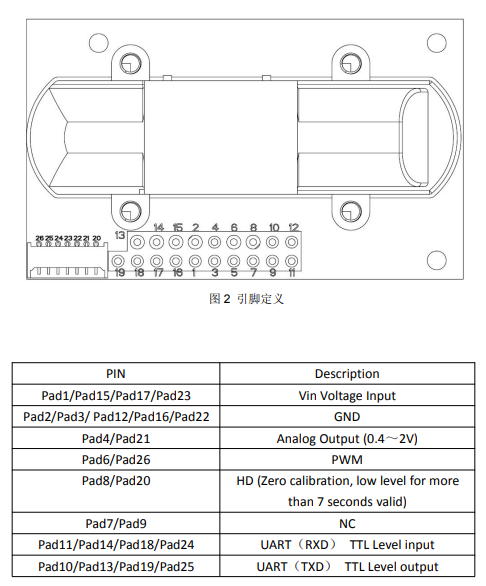
\includegraphics[scale=0.77]{MH-Z14.png}}
	      \end{figure}
	\item \textbf{SDS011}: Módulo de medida de partículas en suspensión, que se conecta mediante USB a la placa.
\end{itemize}

En cuanto a la cámara se usa la Raspberry Pi Camera, más específicamente la \textbf{Ov5647}, que se conecta mediante el puerto CSI directamente a la Raspberry Pi. Esta es la encargada de captar la imagen del CPD en el que se encuentre instalado el dispositivo.

Todas las características técnicas y el porqué de la elección de los sensores y cámara se pueden consultar en la \autoref{subsec:altComponentes}.

Como se puede ver, el elemento central es la \textbf{Raspberry Pi 3B+}, cuyas características se pueden consultar en la \autoref{subsec:altPlacas}. Además, esta se encuentra conectada a la corriente mediante un Micro USB y a la red mediante Ethernet.

Su función es alimentar y acceder a los sensores y cámara, que son los elementos que se encargan de la medición y visualización de la sala, dado que sin la Raspberry estos no serían capaces de funcionar por si solos. Otra de sus funciones clave es la retransmisión de la imagen y el envío de las medidas al servidor. Es por esta razón que se encuentra conectada a la red vía Ethernet.
\chapter{Implementación}
\label{ch:implementacion}
\chapter{Pruebas}
\label{ch:pruebas}
En este capítulo se describen las pruebas que se han realizado en el sistema para comprobar que funciona tal y como se espera, además de verificar que se cumplen satisfactoriamente todas las exigencias del cliente. Muchas de estas pruebas se han efectuado durante la implementación, otras, sin embargo, se han realizado una vez completada, para verificar que en conjunto todo está conectado correctamente.

Las pruebas se abordan desde dos perspectivas: pruebas de caja blanca y pruebas de caja negra. Esto permite que sean más exhaustivas y completas, dado que se trata de un sistema cuyo buen funcionamiento es crítico. 

Cada prueba se recoge de manera tabular siguiendo la plantilla de la \autoref{tab:plantilla_p}.
\begin{table}[H]
	\centering
	\caption{Plantilla de las Pruebas}
	\label{tab:plantilla_p}
	\begin{tabular}{|l|p{.65\textwidth}|}
		\hline
		\multicolumn{2}{|c|}{\cellcolor[HTML]{BFBFBF}{\color[HTML]{000000} \textbf{PCX-YY}}} \\ \hline
		\textbf{Nombre}                  &   \\ \hline
		\textbf{Descripción}             &   \\ \hline
		\textbf{Versión}                 &   \\ \hline
		\textbf{Fuente}                  &   \\ \hline
		\textbf{Proceso}                 &   \\ \hline
		\textbf{Condición de validación} &   \\ \hline
		\textbf{Resultado}               &   \\ \hline
	\end{tabular}
\end{table}
\begin{itemize}
	\item \textbf{PCX-YY:} Identificador de la prueba. Por un lado, la X cambia a B cuando se trata de una prueba de caja blanca y a N cuando es de caja negra. Por otro lado, el YY indica la posición, que aumenta después de cada prueba.
	\item \textbf{Nombre:} Nombre representativo del asunto de la prueba.
	\item \textbf{Descripción:} Exposición más detallada de la prueba.
	\item \textbf{Versión:} Indica si ha sufrido variaciones a lo largo del tiempo.
	\item \textbf{Fuente:} Procedencia del requisito.
	\item \textbf{Proceso:} Acciones a realizar para llevar a cabo la prueba.
	\item \textbf{Condición de validación:} Condiciones que deben cumplirse para que la prueba se dé por superada.
	\item \textbf{Resultado:} Superada, si se da la condición de validación, o Fallida, si no se da.
\end{itemize}

\section{Pruebas de caja blanca}\label{sec:pruebas-de-caja-blanca}
En estas pruebas se verifica el funcionamiento del sistema desde el punto de vista del código fuente desarrollado, de manera que se revise el correcto flujo del programa. Reciben este nombre porque se conoce como se ejecuta el proceso interno. Se presentan a continuación estas pruebas, utilizando la plantilla de la \autoref{tab:plantilla_p}.

\newcount\pcb
\pcb=1
\begin{table}[H]
	\caption{PCB-0\number\pcb}
	\begin{tabular}{|l|p{.65\textwidth}|}
		\hline
		\multicolumn{2}{|c|}{\cellcolor[HTML]{BFBFBF}{\color[HTML]{000000} \textbf{PCB-0\number\pcb}}} \\ \hline
		\textbf{Nombre}                  & IP del dispositivo                                                                        \\ \hline
		\textbf{Descripción}             & Se comprueba el correcto funcionamiento del método \textit{get\_ip()}, que devuelve la IP \\ \hline
		\textbf{Versión}                 & 1.0                                                                                       \\ \hline
		\textbf{Fuente}                  & Responsable de pruebas                                                                    \\ \hline
		\textbf{Proceso}                 & \begin{enumerate}
			\item Hacer una llamada al método \textit{get\_ip()} desde el dispositivo
			\item Hacer \textit{ifconfig} desde el terminal
		\end{enumerate}                                                                 \\ \hline
		\textbf{Condición de validación} & Ambas IP obtenidas deben ser la misma                                                     \\ \hline
		\textbf{Resultado}               & Superada                                                                                  \\ \hline
	\end{tabular}
\end{table}
\advance\pcb by 1
\begin{table}[H]
	\caption{PCB-0\number\pcb}
	\begin{tabular}{|l|p{.65\textwidth}|}
		\hline
		\multicolumn{2}{|c|}{\cellcolor[HTML]{BFBFBF}{\color[HTML]{000000} \textbf{PCB-0\number\pcb}}} \\ \hline
		\textbf{Nombre}                  & id del dispositivo                                                                              \\ \hline
		\textbf{Descripción}             & Se comprueba que el método \textit{get\_device\_id()} devuelve la dirección MAC del dispositivo \\ \hline
		\textbf{Versión}                 & 1.0                                                                                             \\ \hline
		\textbf{Fuente}                  & Responsable de pruebas                                                                          \\ \hline
		\textbf{Proceso}                 & \begin{enumerate}
			\item Crear una llamada en Python a \textit{get\_device\_id()}
			\item Hacer \textit{ifconfig} desde el terminal
		\end{enumerate}                                                                       \\ \hline
		\textbf{Condición de validación} & La dirección MAC obtenida mediante el método debe ser la misma que aparece en el comando        \\ \hline
		\textbf{Resultado}               & Superada                                                                                        \\ \hline
	\end{tabular}
\end{table}
\advance\pcb by 1
\begin{table}[H]
	\caption{PCB-\number\pcb}
	\begin{tabular}{|l|p{.65\textwidth}|}
		\hline
		\multicolumn{2}{|c|}{\cellcolor[HTML]{BFBFBF}{\color[HTML]{000000} \textbf{PCB-\number\pcb}}} \\ \hline
		\textbf{Nombre}                  & Almacenamiento de medidas                                                                    \\ \hline
		\textbf{Descripción}             & Comprobar que las medidas se registran en la tabla \textit{sensor\_data} en la base de datos \\ \hline
		\textbf{Versión}                 & 1.0                                                                                          \\ \hline
		\textbf{Fuente}                  & Responsable de pruebas                                                                       \\ \hline
		\textbf{Proceso}                 & \begin{enumerate}
			\item Acceder a la página de \textit{phpMyAdmin}
			\item Entrar en la base de datos \textit{tfg\_db} y tabla \textit{sensor\_data}
		\end{enumerate}                                                                    \\ \hline
		\textbf{Condición de validación} & Se muestran todas las medidas tomadas                                                        \\ \hline
		\textbf{Resultado}               & Superada                                                                                     \\ \hline
	\end{tabular}
\end{table}
\advance\pcb by 1
\begin{table}[H]
	\caption{PCB-\number\pcb}
	\begin{tabular}{|l|p{.65\textwidth}|}
		\hline
		\multicolumn{2}{|c|}{\cellcolor[HTML]{BFBFBF}{\color[HTML]{000000} \textbf{PCB-\number\pcb}}} \\ \hline
		\textbf{Nombre}                  & Almacenamiento de dispositivos                                                               \\ \hline
		\textbf{Descripción}             & Comprobar que los dispositivos se registran en la tabla \textit{devices} en la base de datos \\ \hline
		\textbf{Versión}                 & 1.0                                                                                          \\ \hline
		\textbf{Fuente}                  & Responsable de pruebas                                                                       \\ \hline
		\textbf{Proceso}                 & \begin{enumerate}
			\item Acceder a la página de \textit{phpMyAdmin}
			\item Entrar en la base de datos \textit{tfg\_db} y tabla \textit{devices}
		\end{enumerate}                                                                    \\ \hline
		\textbf{Condición de validación} & Se muestran todos los dispositivos conectados                                                \\ \hline
		\textbf{Resultado}               & Superada                                                                                     \\ \hline
	\end{tabular}
\end{table}
\advance\pcb by 1
\begin{table}[H]
	\caption{PCB-0\number\pcb}
	\begin{tabular}{|l|p{.65\textwidth}|}
		\hline
		\multicolumn{2}{|c|}{\cellcolor[HTML]{BFBFBF}{\color[HTML]{000000} \textbf{PCB-0\number\pcb}}} \\ \hline
		\textbf{Nombre}                  & Conexión a la base de datos                                                                                                                                                      \\ \hline
		\textbf{Descripción}             & Se comprueba que el dispositivo se conecta correctamente a la base de datos con sus credenciales                                                                                 \\ \hline
		\textbf{Versión}                 & 1.0                                                                                                                                                                              \\ \hline
		\textbf{Fuente}                  & Responsable de pruebas                                                                                                                                                           \\ \hline
		\textbf{Proceso}                 & Crear un objeto de la clase \textit{DB} pasando como parámetros la IP, el usuario "<device\_user">, la contraseña "<device\_pass">, y el nombre de la base de datos "<tfg\_db">. \\ \hline
		\textbf{Condición de validación} & No debe dar error de conexión a la base de datos                                                                                                                                 \\ \hline
		\textbf{Resultado}               & Superada                                                                                                                                                                         \\ \hline
	\end{tabular}
\end{table}
\advance\pcb by 1
\begin{table}[H]
	\caption{PCB-0\number\pcb}
	\begin{tabular}{|l|p{.65\textwidth}|}
		\hline
		\multicolumn{2}{|c|}{\cellcolor[HTML]{BFBFBF}{\color[HTML]{000000} \textbf{PCB-0\number\pcb}}} \\ \hline
		\textbf{Nombre}                  & Añadir dispositivo nuevo                                                                                  \\ \hline
		\textbf{Descripción}             & Se comprueba que se registra correctamente un dispositivo nuevo añadiendo un registro en la base de datos \\ \hline
		\textbf{Versión}                 & 1.0                                                                                                       \\ \hline
		\textbf{Fuente}                  & Responsable de pruebas                                                                                    \\ \hline
		\textbf{Proceso}                 & \begin{enumerate}
			\item Crear un objeto de la clase \textit{DB}
			\item Hacer una llamada al método \textit{insert\_update\_device\_DB()} del objeto, pasando como parámetros: fecha, dirección IP, estado "<Online"> e id del dispositivo
			\item Acceder a la página de \textit{phpMyAdmin}
			\item Entrar en la base de datos \textit{tfg\_db} y tabla \textit{devices}
		\end{enumerate}                                                                                 \\ \hline
		\textbf{Condición de validación} & El dispositivo pasado como parámetro debe estar registrado                                                \\ \hline
		\textbf{Resultado}               & Superada                                                                                                  \\ \hline
	\end{tabular}
\end{table}
\advance\pcb by 1
\begin{table}[H]
	\caption{PCB-0\number\pcb}
	\begin{tabular}{|l|p{.65\textwidth}|}
		\hline
		\multicolumn{2}{|c|}{\cellcolor[HTML]{BFBFBF}{\color[HTML]{000000} \textbf{PCB-0\number\pcb}}} \\ \hline
		\textbf{Nombre}                  & Actualizar dispositivo existente                                                                                                                                                   \\ \hline
		\textbf{Descripción}             & Se comprueba que una vez hay un dispositivo registrado y se hace una llamada al método \textit{insert\_update\_device\_DB()} para el mismo dispositivo, su estado se actualiza \\ \hline
		\textbf{Versión}                 & 1.0                                                                                                                                                                                \\ \hline
		\textbf{Fuente}                  & Responsable de pruebas                                                                                                                                                             \\ \hline
		\textbf{Proceso}                 & \begin{enumerate}
			\item Crear un objeto de la clase \textit{DB}
			\item Hacer una llamada al método \textit{insert\_update\_device\_DB()} del objeto, pasando como parámetros: fecha, dirección IP, estado "<Online"> e id del dispositivo
			\item Llamar al método \textit{insert\_update\_device\_DB()} del objeto, pasando como parámetros: fecha, dirección IP, estado "<Offline"> y el mismo id del dispositivo
			\item Acceder a la página de \textit{phpMyAdmin}
			\item Entrar en la base de datos \textit{tfg\_db} y tabla \textit{devices}
		\end{enumerate}                                                                                                                                                          \\ \hline
		\textbf{Condición de validación} & El registro del dispositivo debe estar actualizado con los parámetros de la segunda llamada                                                                                        \\ \hline
		\textbf{Resultado}               & Superada                                                                                                                                                                           \\ \hline
	\end{tabular}
\end{table}
\advance\pcb by 1
\begin{table}[H]
	\caption{PCB-0\number\pcb}
	\begin{tabular}{|l|p{.65\textwidth}|}
		\hline
		\multicolumn{2}{|c|}{\cellcolor[HTML]{BFBFBF}{\color[HTML]{000000} \textbf{PCB-0\number\pcb}}} \\ \hline
		\textbf{Nombre}                  & Añadir mediciones                                           \\ \hline
		\textbf{Descripción}             & Se comprueba que se registra correctamente la medida tomada \\ \hline
		\textbf{Versión}                 & 1.0                                                         \\ \hline
		\textbf{Fuente}                  & Responsable de pruebas                                      \\ \hline
		\textbf{Proceso}                 & \begin{enumerate}
			\item Crear un objeto de la clase \textit{DB}
			\item Hacer una llamada al método \textit{insert\_sensor\_data\_DB()} del objeto, pasando como parámetros: fecha, id del dispositivo, temperatura, humedad, partículas en suspensión de 2,5, partículas en suspensión de 10, CO y CO$_2$
			\item Acceder a la página de \textit{phpMyAdmin}
			\item Entrar en la base de datos \textit{tfg\_db} y tabla \textit{sensor\_data}
		\end{enumerate}                                  \\ \hline
		\textbf{Condición de validación} & Las medidas pasadas como parámetro deben estar registradas    \\ \hline
		\textbf{Resultado}               & Superada                                                    \\ \hline
	\end{tabular}
\end{table}
\advance\pcb by 1
\begin{table}[H]
	\caption{PCB-0\number\pcb}
	\begin{tabular}{|l|p{.65\textwidth}|}
		\hline
		\multicolumn{2}{|c|}{\cellcolor[HTML]{BFBFBF}{\color[HTML]{000000} \textbf{PCB-0\number\pcb}}} \\ \hline
		\textbf{Nombre}                  & Retransmisión de la cámara                                                                       \\ \hline
		\textbf{Descripción}             & Se comprueba que la imagen de la cámara se muestra en la dirección http://dirIP:8000/stream.mjpg \\ \hline
		\textbf{Versión}                 & 1.0                                                                                              \\ \hline
		\textbf{Fuente}                  & Responsable de pruebas                                                                           \\ \hline
		\textbf{Proceso}                 & \begin{enumerate}
			\item Hacer una llamada al método \textit{cam\_web()}
			\item Acceder a http://dirIP:8000/stream.mjpg
		\end{enumerate}                                                                       \\ \hline
		\textbf{Condición de validación} & La imagen debe estar mostrándose en la página                                                    \\ \hline
		\textbf{Resultado}               & Superada                                                                                         \\ \hline
	\end{tabular}
\end{table}
\advance\pcb by 1
\begin{table}[H]
	\caption{PCB-\number\pcb}
	\begin{tabular}{|l|p{.65\textwidth}|}
		\hline
		\multicolumn{2}{|c|}{\cellcolor[HTML]{BFBFBF}{\color[HTML]{000000} \textbf{PCB-\number\pcb}}} \\ \hline
		\textbf{Nombre}                  & Sensor de temperatura y humedad                                               \\ \hline
		\textbf{Descripción}             & Se comprueba que el sensor de temperatura y humedad funciona                  \\ \hline
		\textbf{Versión}                 & 1.0                                                                           \\ \hline
		\textbf{Fuente}                  & Responsable de pruebas                                                        \\ \hline
		\textbf{Proceso}                 & \begin{enumerate}
			\item Crear un objeto de la clase \textit{DHT11}
			\item Hacer una llamada al método \textit{tempHumSensor()} del objeto
			\item Imprimir la salida por pantalla
		\end{enumerate}                                                    \\ \hline
		\textbf{Condición de validación} & El valor obtenido de la llamada debe concordar con la temperatura del momento \\ \hline
		\textbf{Resultado}               & Superada                                                                      \\ \hline
	\end{tabular}
\end{table}
\advance\pcb by 1
\begin{table}[H]
	\caption{PCB-\number\pcb}
	\begin{tabular}{|l|p{.65\textwidth}|}
		\hline
		\multicolumn{2}{|c|}{\cellcolor[HTML]{BFBFBF}{\color[HTML]{000000} \textbf{PCB-\number\pcb}}} \\ \hline
		\textbf{Nombre}                  & Sensor de partículas en suspensión                                                        \\ \hline
		\textbf{Descripción}             & Se comprueba que el sensor de partículas en suspensión funciona                           \\ \hline
		\textbf{Versión}                 & 1.0                                                                                       \\ \hline
		\textbf{Fuente}                  & Responsable de pruebas                                                                    \\ \hline
		\textbf{Proceso}                 & \begin{enumerate}
			\item Crear un objeto de la clase \textit{SDS011} pasando como parámetro el identificador del puerto USB
			\item Hacer una llamada al método \textit{query()} del objeto
			\item Imprimir la salida por pantalla
		\end{enumerate}                                                                \\ \hline
		\textbf{Condición de validación} & Se deben mostrar por pantalla la cantidad de partículas en suspensión de 2,5 y 10 $\mu m$ \\ \hline
		\textbf{Resultado}               & Superada                                                                                  \\ \hline
	\end{tabular}
\end{table}
\advance\pcb by 1
\begin{table}[H]
	\caption{PCB-\number\pcb}
	\begin{tabular}{|l|p{.65\textwidth}|}
		\hline
		\multicolumn{2}{|c|}{\cellcolor[HTML]{BFBFBF}{\color[HTML]{000000} \textbf{PCB-\number\pcb}}} \\ \hline
		\textbf{Nombre}                  & Sensor de CO$_2$                                                           \\ \hline
		\textbf{Descripción}             & Se comprueba que el sensor de CO$_2$ funciona                              \\ \hline
		\textbf{Versión}                 & 1.0                                                                        \\ \hline
		\textbf{Fuente}                  & Responsable de pruebas                                                     \\ \hline
		\textbf{Proceso}                 & \begin{enumerate}
			\item Crear un objeto de la clase \textit{CO2Sensor}
			\item Hacer una llamada al método \textit{get()} del objeto
			\item Imprimir la salida por pantalla
		\end{enumerate}                                                 \\ \hline
		\textbf{Condición de validación} & Se muestra por pantalla las partículas por millos de CO$_2$ en el ambiente \\ \hline
		\textbf{Resultado}               & Superada                                                                   \\ \hline
	\end{tabular}
\end{table}
\advance\pcb by 1
\begin{table}[H]
	\caption{PCB-\number\pcb}
	\begin{tabular}{|l|p{.65\textwidth}|}
		\hline
		\multicolumn{2}{|c|}{\cellcolor[HTML]{BFBFBF}{\color[HTML]{000000} \textbf{PCB-\number\pcb}}} \\ \hline
		\textbf{Nombre}                  & Sensor de CO                                           \\ \hline
		\textbf{Descripción}             & Se comprueba que el sensor de CO funciona              \\ \hline
		\textbf{Versión}                 & 1.0                                                    \\ \hline
		\textbf{Fuente}                  & Responsable de pruebas                                 \\ \hline
		\textbf{Proceso}                 & \begin{enumerate}
			\item Crear un objeto de la clase \textit{COSensor}
			\item Hacer una llamada al método \textit{co\_sensor\_readadc()} del objeto
			\item Imprimir la salida por pantalla
		\end{enumerate}                             \\ \hline
		\textbf{Condición de validación} & Se muestra por pantalla el porcentaje de CO de la sala \\ \hline
		\textbf{Resultado}               & Superada                                               \\ \hline
	\end{tabular}
\end{table}
\advance\pcb by 1
\begin{table}[H]
	\caption{PCB-\number\pcb}
	\begin{tabular}{|l|p{.65\textwidth}|}
		\hline
		\multicolumn{2}{|c|}{\cellcolor[HTML]{BFBFBF}{\color[HTML]{000000} \textbf{PCB-\number\pcb}}} \\ \hline
		\textbf{Nombre}                  & Funcionamiento general                                                                                                                                                             \\ \hline
		\textbf{Descripción}             & Se comprueba que el programa principal se ejecuta correctamente                                                                                                                    \\ \hline
		\textbf{Versión}                 & 1.0                                                                                                                                                                                \\ \hline
		\textbf{Fuente}                  & Responsable de pruebas                                                                                                                                                             \\ \hline
		\textbf{Proceso}                 & \begin{enumerate}
			\item Llamar al método \textit{cpdDevice()} del programa principal
			\item Esperar 20 segundos a que se calienten los sensores
			\item Observar el terminal durante 1 minuto
			\item Acceder a la página de \textit{phpMyAdmin}
			\item Entrar en la base de datos \textit{tfg\_db} y tabla \textit{sensor\_data}
			\item Entrar en la base de datos \textit{tfg\_db} y tabla \textit{devices}
		\end{enumerate}                                                                                                                                                         \\ \hline
		\textbf{Condición de validación} & En el terminal se muestran cada 5 segundos las medidas tomadas, que coinciden con las de la tabla \textit{sensor\_data}. Además, el dispositivo debe mostrarse en \textit{devices} \\ \hline
		\textbf{Resultado}               & Superada                                                                                                                                                                           \\ \hline
	\end{tabular}
\end{table}
\vspace{-1cm}

\section{Pruebas de caja negra}\label{sec:pruebas-de-caja-negra}
En esta sección se efectúan las pruebas relativas al correcto funcionamiento del sistema en general, sin entrar en cómo funciona internamente, es por esto por lo que se llaman pruebas de caja negra. Las pruebas hechas se muestran en las siguientes tablas, que siguen la plantilla de la \autoref{tab:plantilla_p}.
\newcount\pcn
\pcn=1
\begin{table}[H]
	\caption{PCN-0\number\pcn}
	\begin{tabular}{|l|p{.65\textwidth}|}
		\hline
		\multicolumn{2}{|c|}{\cellcolor[HTML]{BFBFBF}{\color[HTML]{000000} \textbf{PCN-0\number\pcn}}} \\ \hline
		\textbf{Nombre}                  & Acceso a la web                                                            \\ \hline
		\textbf{Descripción}             & Comprobar que se puede acceder a la aplicación                             \\ \hline
		\textbf{Versión}                 & 1.0                                                                        \\ \hline
		\textbf{Fuente}                  & Responsable de pruebas                                                     \\ \hline
		\textbf{Proceso}                 & Se introduce el enlace de la aplicación en un navegador                    \\ \hline
		\textbf{Condición de validación} & Muestra el inicio de sesión de la aplicación, con una paleta de azules \\ \hline
		\textbf{Resultado}               & Superada                                                                   \\ \hline
	\end{tabular}
\end{table}
\advance\pcn by 1
\begin{table}[H]
	\caption{PCN-0\number\pcn}
	\begin{tabular}{|l|p{.65\textwidth}|}
		\hline
		\multicolumn{2}{|c|}{\cellcolor[HTML]{BFBFBF}{\color[HTML]{000000} \textbf{PCN-0\number\pcn}}} \\ \hline
		\textbf{Nombre}                  & Registrar usuario                                                                                                 \\ \hline
		\textbf{Descripción}             & Comprobar el proceso de registro del administrador                                                                \\ \hline
		\textbf{Versión}                 & 1.0                                                                                                               \\ \hline
		\textbf{Fuente}                  & Responsable de pruebas                                                                                            \\ \hline
		\textbf{Proceso}                 & Hacer en la base de datos una query de inserción a la tabla \textit{users}, indicando usuario y contraseña en MD5 \\ \hline
		\textbf{Condición de validación} & Se puede acceder a la aplicación con el usuario recién creado                                                     \\ \hline
		\textbf{Resultado}               & Superada                                                                                                          \\ \hline
	\end{tabular}
\end{table}
\advance\pcn by 1
\begin{table}[H]
	\caption{PCN-0\number\pcn}
	\begin{tabular}{|l|p{.65\textwidth}|}
		\hline
		\multicolumn{2}{|c|}{\cellcolor[HTML]{BFBFBF}{\color[HTML]{000000} \textbf{PCN-0\number\pcn}}} \\ \hline
		\textbf{Nombre}                  & Acceso a la aplicación                                              \\ \hline
		\textbf{Descripción}             & Se comprueba que la web es accesible mediante un usuario registrado \\ \hline
		\textbf{Versión}                 & 1.0                                                                 \\ \hline
		\textbf{Fuente}                  & Responsable de pruebas                                              \\ \hline
		\textbf{Proceso}                 & \begin{enumerate}
			\item Acceder a la aplicación web
			\item Introducir las credenciales de usuario de un registro de la tabla \textit{users}
		\end{enumerate}                                          \\ \hline
		\textbf{Condición de validación} & Se accede a la aplicación satisfactoriamente                        \\ \hline
		\textbf{Resultado}               & Superada                                                            \\ \hline
	\end{tabular}
\end{table}
\advance\pcn by 1
\begin{table}[H]
	\caption{PCN-0\number\pcn}
	\begin{tabular}{|l|p{.65\textwidth}|}
		\hline
		\multicolumn{2}{|c|}{\cellcolor[HTML]{BFBFBF}{\color[HTML]{000000} \textbf{PCN-0\number\pcn}}} \\ \hline
		\textbf{Nombre}                  & Cierre de sesión                                                    \\ \hline
		\textbf{Descripción}             & Se comprueba que se borra la sesión y se vuelve al inicio de sesión \\ \hline
		\textbf{Versión}                 & 1.0                                                                 \\ \hline
		\textbf{Fuente}                  & Responsable de pruebas                                              \\ \hline
		\textbf{Proceso}                 & \begin{enumerate}
			\item Acceder a la aplicación web
			\item Iniciar sesión
			\item Clic en "<Cerrar sesión">
		\end{enumerate}                                          \\ \hline
		\textbf{Condición de validación} & Se vuelve a la página de inicio de sesión                           \\ \hline
		\textbf{Resultado}               & Superada                                                            \\ \hline
	\end{tabular}
\end{table}
\advance\pcn by 1
\begin{table}[H]
	\caption{PCN-0\number\pcn}
	\begin{tabular}{|l|p{.65\textwidth}|}
		\hline
		\multicolumn{2}{|c|}{\cellcolor[HTML]{BFBFBF}{\color[HTML]{000000} \textbf{PCN-0\number\pcn}}} \\ \hline
		\textbf{Nombre}                  & Bienvenida a la web                     \\ \hline
		\textbf{Descripción}             & Se muestra el usuario al iniciar sesión \\ \hline
		\textbf{Versión}                 & 1.0                                     \\ \hline
		\textbf{Fuente}                  & Responsable de pruebas                  \\ \hline
		\textbf{Proceso}                 & \begin{enumerate}
			\item Acceder a la aplicación web
			\item Iniciar sesión
		\end{enumerate}              \\ \hline
		\textbf{Condición de validación} & Se muestra el nombre de usuario         \\ \hline
		\textbf{Resultado}               & Superada                                \\ \hline
	\end{tabular}
\end{table}
\advance\pcn by 1
\begin{table}[H]
	\caption{PCN-0\number\pcn}
	\begin{tabular}{|l|p{.65\textwidth}|}
		\hline
		\multicolumn{2}{|c|}{\cellcolor[HTML]{BFBFBF}{\color[HTML]{000000} \textbf{PCN-0\number\pcn}}} \\ \hline
		\textbf{Nombre}                  & Lista de dispositivos                                          \\ \hline
		\textbf{Descripción}             & Comprobar que se muestran los dispositivos en la aplicación    \\ \hline
		\textbf{Versión}                 & 1.0                                                            \\ \hline
		\textbf{Fuente}                  & Responsable de pruebas                                         \\ \hline
		\textbf{Proceso}                 & \begin{enumerate}
			\item Acceder a la aplicación web
			\item Iniciar sesión
		\end{enumerate}                                     \\ \hline
		\textbf{Condición de validación} & Se deben mostrar los dispositivos de la tabla \textit{devices} \\ \hline
		\textbf{Resultado}               & Superada                                                       \\ \hline
	\end{tabular}
\end{table}
\advance\pcn by 1
\begin{table}[H]
	\caption{PCN-0\number\pcn}
	\begin{tabular}{|l|p{.65\textwidth}|}
		\hline
		\multicolumn{2}{|c|}{\cellcolor[HTML]{BFBFBF}{\color[HTML]{000000} \textbf{PCN-0\number\pcn}}} \\ \hline
		\textbf{Nombre}                  & Acceso a la página de dispositivo                                            \\ \hline
		\textbf{Descripción}             & Se comprueba que se muestra la imagen y medidas del dispositivo seleccionado \\ \hline
		\textbf{Versión}                 & 1.0                                                                          \\ \hline
		\textbf{Fuente}                  & Responsable de pruebas                                                       \\ \hline
		\textbf{Proceso}                 & \begin{enumerate}
			\item Acceder a la aplicación web
			\item Iniciar sesión
			\item Hacer clic en "<Acceder"> en la lista de dispositivos
		\end{enumerate}                                                   \\ \hline
		\textbf{Condición de validación} & Deben aparecer las medidas e imagen                                          \\ \hline
		\textbf{Resultado}               & Superada                                                                     \\ \hline
	\end{tabular}
\end{table}
\advance\pcn by 1
\begin{table}[H]
	\caption{PCN-0\number\pcn}
	\begin{tabular}{|l|p{.65\textwidth}|}
		\hline
		\multicolumn{2}{|c|}{\cellcolor[HTML]{BFBFBF}{\color[HTML]{000000} \textbf{PCN-0\number\pcn}}} \\ \hline
		\textbf{Nombre}                  & Acceso a medidas del dispositivo                    \\ \hline
		\textbf{Descripción}             & Comprobar que las medidas tomadas se muestran       \\ \hline
		\textbf{Versión}                 & 1.0                                                 \\ \hline
		\textbf{Fuente}                  & Responsable de pruebas                              \\ \hline
		\textbf{Proceso}                 & \begin{enumerate}
			\item Acceder a la aplicación web
			\item Iniciar sesión
			\item Hacer clic en "<Acceder"> en la lista de dispositivos
		\end{enumerate}                          \\ \hline
		\textbf{Condición de validación} & Deben aparecer las medidas tomadas en tabla y lista \\ \hline
		\textbf{Resultado}               & Superada                                            \\ \hline
	\end{tabular}
\end{table}
\advance\pcn by 1
\begin{table}[H]
	\caption{PCN-0\number\pcn}
	\begin{tabular}{|l|p{.65\textwidth}|}
		\hline
		\multicolumn{2}{|c|}{\cellcolor[HTML]{BFBFBF}{\color[HTML]{000000} \textbf{PCN-0\number\pcn}}} \\ \hline
		\textbf{Nombre}                  & Acceso a la imagen del dispositivo              \\ \hline
		\textbf{Descripción}             & Comprobar que la imagen de la cámara se muestra \\ \hline
		\textbf{Versión}                 & 1.0                                             \\ \hline
		\textbf{Fuente}                  & Responsable de pruebas                          \\ \hline
		\textbf{Proceso}                 & \begin{enumerate}
			\item Acceder a la aplicación web
			\item Iniciar sesión
			\item Hacer clic en "<Acceder"> en la lista de dispositivos
		\end{enumerate}                      \\ \hline
		\textbf{Condición de validación} & Debe aparecer la imagen en tiempo real          \\ \hline
		\textbf{Resultado}               & Superada                                        \\ \hline
	\end{tabular}
\end{table}
\advance\pcn by 1
\begin{table}[H]
	\caption{PCN-\number\pcn}
	\begin{tabular}{|l|p{.65\textwidth}|}
		\hline
		\multicolumn{2}{|c|}{\cellcolor[HTML]{BFBFBF}{\color[HTML]{000000} \textbf{PCN-\number\pcn}}} \\ \hline
		\textbf{Nombre}                  & Volver a la lista de dispositivos                                                              \\ \hline
		\textbf{Descripción}             & Se comprueba que al hacer clic en "<Volver"> se vuelve a la página de selección de dispositivo \\ \hline
		\textbf{Versión}                 & 1.0                                                                                            \\ \hline
		\textbf{Fuente}                  & Responsable de pruebas                                                                         \\ \hline
		\textbf{Proceso}                 & \begin{enumerate}
			\item Acceder a la aplicación web
			\item Iniciar sesión
			\item Hacer clic en "<Acceder"> en la lista de dispositivos
			\item Hacer clic en "<Volver">
		\end{enumerate}                                                                     \\ \hline
		\textbf{Condición de validación} & Se vuelve a la lista de dispositivos                                                           \\ \hline
		\textbf{Resultado}               & Superada                                                                                       \\ \hline
	\end{tabular}
\end{table}
\advance\pcn by 1
\begin{table}[H]
	\caption{PCN-\number\pcn}
	\begin{tabular}{|l|p{.65\textwidth}|}
		\hline
		\multicolumn{2}{|c|}{\cellcolor[HTML]{BFBFBF}{\color[HTML]{000000} \textbf{PCN-\number\pcn}}} \\ \hline
		\textbf{Nombre}                  & Funcionamiento continuado                                                                       \\ \hline
		\textbf{Descripción}             & Dejar el dispositivo funcionando sin cortes                                                     \\ \hline
		\textbf{Versión}                 & 1.0                                                                                             \\ \hline
		\textbf{Fuente}                  & Responsable de pruebas                                                                          \\ \hline
		\textbf{Proceso}                 & Dejar funcionando el dispositivo 7 días, revisando periódicamente                               \\ \hline
		\textbf{Condición de validación} & No se corta la imagen en ningún momento, ni se cae la aplicación y las medias no se interrumpen \\ \hline
		\textbf{Resultado}               & Superada                                                                                        \\ \hline
	\end{tabular}
\end{table}
\advance\pcn by 1
\begin{table}[H]
	\caption{PCN-\number\pcn}
	\begin{tabular}{|l|p{.65\textwidth}|}
		\hline
		\multicolumn{2}{|c|}{\cellcolor[HTML]{BFBFBF}{\color[HTML]{000000} \textbf{PCN-\number\pcn}}} \\ \hline
		\textbf{Nombre}                  & Responsive                                              \\ \hline
		\textbf{Descripción}             & Navegar por la aplicación en versión escritorio y móvil \\ \hline
		\textbf{Versión}                 & 1.0                                                     \\ \hline
		\textbf{Fuente}                  & Responsable de pruebas                                  \\ \hline
		\textbf{Proceso}                 & \begin{enumerate}
			\item Activar versión desktop en DevTools
			\item Iniciar sesión
			\item Seleccionar dispositivo
			\item Volver a la lista de dispositivos
			\item Cerrar sesión
			\item Activar versión móvil en DevTools
			\item Iniciar sesión
			\item Seleccionar dispositivo
		\end{enumerate}                              \\ \hline
		\textbf{Condición de validación} & En todo momento debe ser perfectamente navegable        \\ \hline
		\textbf{Resultado}               & Superada                                                \\ \hline
	\end{tabular}
\end{table}
\pagebreak

\section{Matriz de trazabilidad}\label{sec:matriz-de-trazabilidad}
La intención de esta sección es poder verificar que todos los requisitos que ha exigido el cliente quedan cubiertos por las pruebas.

Se emplea la misma representación que se explica en la \autoref{sec:matrizAnalisis}, una matriz de trazabilidad, pero en este caso se relacionan los requisitos de usuario (filas) con las pruebas (columnas). Esta matriz se encuentra dividida en la \autoref{tab:trazabilidadPI}, \autoref{tab:trazabilidadPII} y \autoref{tab:trazabilidadPIII}.

\begin{table}[H]
	\centering
	\caption{Matriz de trazabilidad de pruebas I}
	\label{tab:trazabilidadPI}
	\resizebox{\textwidth}{!}{%
		\begin{tabular}{|
				>{\columncolor[HTML]{BFBFBF}}l |c|c|c|c|c|c|c|c|c|}
			\hline
			\textbf{RF N \textbackslash{}RU} & \cellcolor[HTML]{BFBFBF}\textbf{PCB-01} & \cellcolor[HTML]{BFBFBF}\textbf{PCB-02} & \cellcolor[HTML]{BFBFBF}\textbf{PCB-03} & \cellcolor[HTML]{BFBFBF}\textbf{PCB-04} & \cellcolor[HTML]{BFBFBF}\textbf{PCB-05} & \cellcolor[HTML]{BFBFBF}\textbf{PCB-06} & \cellcolor[HTML]{BFBFBF}\textbf{PCB-07} & \cellcolor[HTML]{BFBFBF}\textbf{PCB-08} & \cellcolor[HTML]{BFBFBF}\textbf{PCB-09} \\ \hline
			\textbf{RF-01}                   &                                         &                                         & X                                       &                                         & X                                       &                                         &                                         & X                                       &                                         \\ \hline
			\textbf{RF-02}                   &                                         &                                         & X                                       &                                         & X                                       &                                         &                                         & X                                       &                                         \\ \hline
			\textbf{RF-03}                   &                                         &                                         &                                         &                                         &                                         &                                         &                                         &                                         & X                                       \\ \hline
			\textbf{RF-04}                   &                                         &                                         &                                         &                                         &                                         &                                         &                                         &                                         &                                         \\ \hline
			\textbf{RF-05}                   &                                         &                                         &                                         &                                         &                                         &                                         &                                         &                                         &                                         \\ \hline
			\textbf{RF-06}                   &                                         &                                         &                                         &                                         &                                         &                                         &                                         &                                         &                                         \\ \hline
			\textbf{RF-07}                   &                                         &                                         &                                         &                                         &                                         &                                         &                                         &                                         &                                         \\ \hline
			\textbf{RF-08}                   &                                         &                                         &                                         &                                         &                                         &                                         &                                         &                                         &                                         \\ \hline
			\textbf{RF-09}                   &                                         &                                         &                                         &                                         &                                         &                                         &                                         &                                         &                                         \\ \hline
			\textbf{RF-10}                   &                                         &                                         &                                         &                                         &                                         &                                         &                                         &                                         &                                         \\ \hline
			\textbf{RF-11}                   &                                         &                                         &                                         &                                         &                                         &                                         &                                         &                                         &                                         \\ \hline
			\textbf{RF-12}                   &                                         &                                         &                                         &                                         &                                         &                                         &                                         &                                         &                                         \\ \hline
			\textbf{RF-13}                   &                                         &                                         &                                         &                                         &                                         &                                         &                                         &                                         &                                         \\ \hline
			\textbf{RN-01}                   &                                         &                                         &                                         &                                         &                                         &                                         &                                         &                                         &                                         \\ \hline
			\textbf{RN-02}                   &                                         &                                         &                                         &                                         &                                         &                                         &                                         &                                         &                                         \\ \hline
			\textbf{RN-03}                   &                                         &                                         &                                         &                                         &                                         &                                         &                                         &                                         &                                         \\ \hline
			\textbf{RN-04}                   &                                         &                                         &                                         &                                         &                                         &                                         &                                         &                                         &                                         \\ \hline
			\textbf{RN-05}                   &                                         &                                         &                                         &                                         &                                         &                                         &                                         &                                         &                                         \\ \hline
			\textbf{RN-06}                   &                                         &                                         &                                         &                                         &                                         &                                         &                                         &                                         & X                                       \\ \hline
			\textbf{RN-07}                   &                                         &                                         &                                         &                                         &                                         &                                         &                                         &                                         &                                         \\ \hline
			\textbf{RN-08}                   & X                                       & X                                       & X                                       & X                                       & X                                       &                                         &                                         &                                         & X                                       \\ \hline
			\textbf{RN-09}                   &                                         &                                         &                                         &                                         &                                         &                                         &                                         &                                         &                                         \\ \hline
			\textbf{RN-10}                   &                                         &                                         & X                                       & X                                       & X                                       & X                                       & X                                       & X                                       &                                         \\ \hline
			\textbf{RN-11}                   &                                         &                                         & X                                       &                                         &                                         &                                         &                                         &                                         &                                         \\ \hline
			\textbf{RN-12}                   &                                         &                                         &                                         &                                         &                                         &                                         &                                         &                                         &                                         \\ \hline
			\textbf{RN-13}                   &                                         &                                         &                                         &                                         &                                         &                                         &                                         & X                                       &                                         \\ \hline
			\textbf{RN-14}                   &                                         &                                         &                                         &                                         &                                         &                                         &                                         &                                         &                                         \\ \hline
			\textbf{RN-15}                   &                                         &                                         &                                         &                                         &                                         &                                         &                                         &                                         & X                                       \\ \hline
			\textbf{RN-16}                   &                                         &                                         &                                         &                                         &                                         &                                         &                                         &                                         &                                         \\ \hline
			\textbf{RN-17}                   &                                         &                                         &                                         &                                         &                                         &                                         &                                         &                                         &                                         \\ \hline
			\textbf{RN-18}                   &                                         &                                         &                                         &                                         &                                         &                                         &                                         &                                         &                                         \\ \hline
			\textbf{RN-19}                   & X                                       & X                                       &                                         & X                                       &                                         &                                         &                                         &                                         &                                         \\ \hline
			\textbf{RN-20}                   &                                         &                                         &                                         &                                         &                                         & X                                       & X                                       &                                         &                                         \\ \hline
			\textbf{RN-21}                   &                                         &                                         &                                         &                                         &                                         &                                         &                                         &                                         &                                         \\ \hline
			\textbf{RN-22}                   &                                         &                                         &                                         &                                         &                                         &                                         &                                         &                                         &                                         \\ \hline
			\textbf{RN-23}                   &                                         &                                         &                                         &                                         &                                         &                                         &                                         &                                         &                                         \\ \hline
			\textbf{RN-24}                   &                                         &                                         &                                         &                                         &                                         &                                         &                                         &                                         &                                         \\ \hline
		\end{tabular}%
	}
\end{table}

\begin{table}[H]
	\centering
	\caption{Matriz de trazabilidad de pruebas II}
	\label{tab:trazabilidadPII}
	\resizebox{\textwidth}{!}{%
		\begin{tabular}{|
				>{\columncolor[HTML]{BFBFBF}}l |c|c|c|c|c|c|c|c|c|}
			\hline
			\textbf{RF N \textbackslash{}RU} & \cellcolor[HTML]{BFBFBF}\textbf{PCB-10} & \cellcolor[HTML]{BFBFBF}\textbf{PCB-11} & \cellcolor[HTML]{BFBFBF}\textbf{PCB-12} & \cellcolor[HTML]{BFBFBF}\textbf{PCB-13} & \cellcolor[HTML]{BFBFBF}\textbf{PCB-14} & \cellcolor[HTML]{BFBFBF}\textbf{PCN-01} & \cellcolor[HTML]{BFBFBF}\textbf{PCN-02} & \cellcolor[HTML]{BFBFBF}\textbf{PCN-03} & \cellcolor[HTML]{BFBFBF}\textbf{PCN-04} \\ \hline
			\textbf{RF-01}                   & X                                       & X                                       & X                                       & X                                       &                                         &                                         &                                         &                                         &                                         \\ \hline
			\textbf{RF-02}                   & X                                       & X                                       & X                                       & X                                       &                                         &                                         &                                         &                                         &                                         \\ \hline
			\textbf{RF-03}                   &                                         &                                         &                                         &                                         &                                         &                                         &                                         &                                         &                                         \\ \hline
			\textbf{RF-04}                   &                                         &                                         &                                         &                                         &                                         &                                         & X                                       &                                         &                                         \\ \hline
			\textbf{RF-05}                   &                                         &                                         &                                         &                                         &                                         &                                         &                                         & X                                       &                                         \\ \hline
			\textbf{RF-06}                   &                                         &                                         &                                         &                                         &                                         &                                         &                                         &                                         &                                         \\ \hline
			\textbf{RF-07}                   &                                         &                                         &                                         &                                         &                                         &                                         &                                         &                                         & X                                       \\ \hline
			\textbf{RF-08}                   &                                         &                                         &                                         &                                         &                                         &                                         &                                         &                                         &                                         \\ \hline
			\textbf{RF-09}                   &                                         &                                         &                                         &                                         &                                         & X                                       &                                         &                                         &                                         \\ \hline
			\textbf{RF-10}                   &                                         &                                         &                                         &                                         &                                         &                                         &                                         &                                         &                                         \\ \hline
			\textbf{RF-11}                   &                                         &                                         &                                         &                                         &                                         &                                         &                                         &                                         &                                         \\ \hline
			\textbf{RF-12}                   &                                         &                                         &                                         &                                         &                                         &                                         &                                         &                                         &                                         \\ \hline
			\textbf{RF-13}                   &                                         &                                         &                                         &                                         &                                         &                                         &                                         &                                         &                                         \\ \hline
			\textbf{RN-01}                   & X                                       &                                         &                                         &                                         &                                         &                                         &                                         &                                         &                                         \\ \hline
			\textbf{RN-02}                   & X                                       &                                         &                                         &                                         &                                         &                                         &                                         &                                         &                                         \\ \hline
			\textbf{RN-03}                   &                                         &                                         &                                         & X                                       &                                         &                                         &                                         &                                         &                                         \\ \hline
			\textbf{RN-04}                   &                                         &                                         & X                                       &                                         &                                         &                                         &                                         &                                         &                                         \\ \hline
			\textbf{RN-05}                   &                                         & X                                       &                                         &                                         &                                         &                                         &                                         &                                         &                                         \\ \hline
			\textbf{RN-06}                   &                                         &                                         &                                         &                                         &                                         &                                         &                                         &                                         &                                         \\ \hline
			\textbf{RN-07}                   &                                         &                                         &                                         &                                         &                                         &                                         &                                         &                                         &                                         \\ \hline
			\textbf{RN-08}                   &                                         &                                         &                                         &                                         &                                         &                                         &                                         &                                         &                                         \\ \hline
			\textbf{RN-09}                   &                                         &                                         &                                         &                                         & X                                       &                                         &                                         &                                         &                                         \\ \hline
			\textbf{RN-10}                   &                                         &                                         &                                         &                                         &                                         & X                                       &                                         &                                         &                                         \\ \hline
			\textbf{RN-11}                   &                                         &                                         &                                         &                                         &                                         &                                         &                                         &                                         &                                         \\ \hline
			\textbf{RN-12}                   &                                         &                                         &                                         &                                         & X                                       &                                         &                                         &                                         &                                         \\ \hline
			\textbf{RN-13}                   &                                         &                                         &                                         &                                         &                                         &                                         &                                         &                                         &                                         \\ \hline
			\textbf{RN-14}                   &                                         &                                         &                                         &                                         &                                         &                                         &                                         &                                         &                                         \\ \hline
			\textbf{RN-15}                   &                                         &                                         &                                         &                                         &                                         &                                         &                                         &                                         &                                         \\ \hline
			\textbf{RN-16}                   &                                         &                                         &                                         &                                         &                                         &                                         & X                                       & X                                       &                                         \\ \hline
			\textbf{RN-17}                   &                                         &                                         &                                         &                                         &                                         &                                         & X                                       &                                         &                                         \\ \hline
			\textbf{RN-18}                   &                                         &                                         &                                         &                                         &                                         &                                         & X                                       &                                         &                                         \\ \hline
			\textbf{RN-19}                   &                                         &                                         &                                         &                                         &                                         &                                         &                                         &                                         &                                         \\ \hline
			\textbf{RN-20}                   &                                         &                                         &                                         &                                         &                                         &                                         &                                         &                                         &                                         \\ \hline
			\textbf{RN-21}                   &                                         &                                         &                                         &                                         &                                         & X                                       &                                         & X                                       &                                         \\ \hline
			\textbf{RN-22}                   &                                         &                                         &                                         &                                         &                                         &                                         &                                         &                                         &                                         \\ \hline
			\textbf{RN-23}                   &                                         &                                         &                                         &                                         &                                         &                                         &                                         &                                         &                                         \\ \hline
			\textbf{RN-24}                   &                                         &                                         &                                         &                                         &                                         &                                         &                                         &                                         &                                         \\ \hline
		\end{tabular}%
	}
\end{table}

\begin{table}[H]
	\centering
	\caption{Matriz de trazabilidad de pruebas III}
	\label{tab:trazabilidadPIII}
	\resizebox{\textwidth}{!}{%
		\begin{tabular}{|
				>{\columncolor[HTML]{BFBFBF}}l |c|c|c|c|c|c|c|c|}
			\hline
			\textbf{RF N \textbackslash{}RU} & \cellcolor[HTML]{BFBFBF}\textbf{PCN-05} & \cellcolor[HTML]{BFBFBF}\textbf{PCN-06} & \cellcolor[HTML]{BFBFBF}\textbf{PCN-07} & \cellcolor[HTML]{BFBFBF}\textbf{PCN-08} & \cellcolor[HTML]{BFBFBF}\textbf{PCN-09} & \cellcolor[HTML]{BFBFBF}\textbf{PCN-10} & \cellcolor[HTML]{BFBFBF}\textbf{PCN-11} & \cellcolor[HTML]{BFBFBF}\textbf{PCN-12} \\ \hline
			\textbf{RF-01}                   &                                         &                                         & X                                       & X                                       &                                         &                                         &                                         &                                         \\ \hline
			\textbf{RF-02}                   &                                         &                                         & X                                       & X                                       &                                         &                                         &                                         &                                         \\ \hline
			\textbf{RF-03}                   &                                         &                                         &                                         &                                         & X                                       &                                         &                                         &                                         \\ \hline
			\textbf{RF-04}                   &                                         &                                         &                                         &                                         &                                         &                                         &                                         &                                         \\ \hline
			\textbf{RF-05}                   &                                         &                                         &                                         &                                         &                                         &                                         &                                         &                                         \\ \hline
			\textbf{RF-06}                   &                                         & X                                       &                                         &                                         &                                         &                                         &                                         &                                         \\ \hline
			\textbf{RF-07}                   &                                         &                                         &                                         &                                         &                                         &                                         &                                         &                                         \\ \hline
			\textbf{RF-08}                   & X                                       &                                         &                                         &                                         &                                         &                                         &                                         &                                         \\ \hline
			\textbf{RF-09}                   &                                         &                                         &                                         &                                         &                                         &                                         &                                         &                                         \\ \hline
			\textbf{RF-10}                   &                                         &                                         & X                                       & X                                       & X                                       &                                         &                                         &                                         \\ \hline
			\textbf{RF-11}                   &                                         &                                         &                                         &                                         &                                         & X                                       &                                         &                                         \\ \hline
			\textbf{RF-12}                   &                                         &                                         & X                                       & X                                       &                                         &                                         &                                         &                                         \\ \hline
			\textbf{RF-13}                   &                                         &                                         & X                                       & X                                       &                                         &                                         &                                         &                                         \\ \hline
			\textbf{RN-01}                   &                                         &                                         &                                         &                                         &                                         &                                         &                                         &                                         \\ \hline
			\textbf{RN-02}                   &                                         &                                         &                                         &                                         &                                         &                                         &                                         &                                         \\ \hline
			\textbf{RN-03}                   &                                         &                                         &                                         &                                         &                                         &                                         &                                         &                                         \\ \hline
			\textbf{RN-04}                   &                                         &                                         &                                         &                                         &                                         &                                         &                                         &                                         \\ \hline
			\textbf{RN-05}                   &                                         &                                         &                                         &                                         &                                         &                                         &                                         &                                         \\ \hline
			\textbf{RN-06}                   &                                         &                                         &                                         &                                         &                                         &                                         &                                         &                                         \\ \hline
			\textbf{RN-07}                   &                                         &                                         &                                         &                                         &                                         &                                         & X                                       &                                         \\ \hline
			\textbf{RN-08}                   &                                         &                                         &                                         &                                         &                                         &                                         &                                         &                                         \\ \hline
			\textbf{RN-09}                   &                                         &                                         &                                         &                                         &                                         &                                         &                                         &                                         \\ \hline
			\textbf{RN-10}                   &                                         &                                         &                                         &                                         &                                         &                                         &                                         &                                         \\ \hline
			\textbf{RN-11}                   &                                         &                                         &                                         &                                         &                                         &                                         &                                         &                                         \\ \hline
			\textbf{RN-12}                   &                                         &                                         &                                         &                                         &                                         &                                         &                                         &                                         \\ \hline
			\textbf{RN-13}                   &                                         &                                         &                                         &                                         &                                         &                                         &                                         &                                         \\ \hline
			\textbf{RN-14}                   &                                         &                                         & X                                       & X                                       & X                                       &                                         &                                         &                                         \\ \hline
			\textbf{RN-15}                   &                                         &                                         &                                         &                                         &                                         &                                         &                                         &                                         \\ \hline
			\textbf{RN-16}                   &                                         &                                         &                                         &                                         &                                         &                                         &                                         &                                         \\ \hline
			\textbf{RN-17}                   &                                         &                                         &                                         &                                         &                                         &                                         &                                         &                                         \\ \hline
			\textbf{RN-18}                   &                                         &                                         &                                         &                                         &                                         &                                         &                                         &                                         \\ \hline
			\textbf{RN-19}                   &                                         &                                         &                                         &                                         &                                         &                                         &                                         &                                         \\ \hline
			\textbf{RN-20}                   &                                         &                                         &                                         &                                         &                                         &                                         &                                         &                                         \\ \hline
			\textbf{RN-21}                   &                                         & X                                       & X                                       &                                         &                                         &                                         &                                         &                                         \\ \hline
			\textbf{RN-22}                   &                                         &                                         &                                         &                                         &                                         &                                         &                                         & X                                       \\ \hline
			\textbf{RN-23}                   &                                         &                                         &                                         &                                         &                                         &                                         & X                                       &                                         \\ \hline
			\textbf{RN-24}                   &                                         &                                         &                                         &                                         &                                         &                                         & X                                       &                                         \\ \hline
		\end{tabular}%
	}
\end{table}
\chapter{Gestión del proyecto}
\label{ch:gestion}
\section{Planificación}
EXPLICAR LOS PLAZOS DEL PROYECTO Y DECIR QUE SE HA DISTRIBUIDO EN EL TIEMPO COMO SE INDICARA EN LA SIGUIENTE SECCIÓN

\subsection{Desglose por fases}
EXPLICAR BREVEMENTE LAS FASES Y PONER TABLA DE FASES

\subsection{Diagrama de Gantt}
EXPLICAR QUE NOS APOYAMOS EN ESTA REPRESENTACIÓN DAR CLARIDAD

\ganttset{calendar week text= \small {\startday/\startmonth}}
\begin{figure}[H]
  \ffigbox[\FBwidth]
  {\caption{Diagrama de Gantt}} % Hasta determinar fechas se ha puesto 27-06-2021 que no se utiliza para facilitar el remplazo
  {\resizebox{\textwidth}{!}{%
      \begin{ganttchart}[
        x unit=1.5mm,
        time slot format=little-endian,
        hgrid style/.style={dotted, line width=.75pt},
        vgrid={*6{draw=black!5, line width=.75pt},*1{dash pattern=on 3.5pt off 4.5pt}},
        bar label font=\mdseries\small\color{black!70},
        bar/.append style={draw=none, fill=ganttblue},
        group left shift=0,
        group right shift=0,
        group peaks tip position=0,
        ]{21-06-2021}{16-1-2022}
        \gantttitlecalendar{year, month=name, week} \\[grid]
        
        \ganttbar{Propuesta}{29-06-2021}{23-07-2021}\\[grid]
        
        \ganttbar{Documentación previa}{15-07-2021}{03-08-2021}\\[grid]
        
        \ganttgroup{Introducción}{27-06-2021}{27-06-2021}\\
        \ganttbar{Motivación}{27-06-2021}{27-06-2021}\\
        \ganttbar{Objetivos}{27-06-2021}{27-06-2021}\\
        \ganttbar{Metodología}{27-06-2021}{27-06-2021}\\[grid]
        
        \ganttgroup{Estado del arte}{27-06-2021}{27-06-2021}\\
        \ganttbar{Soluciones actuales}{27-06-2021}{27-06-2021}\\
        \ganttbar{Critica al estado del arte}{27-06-2021}{27-06-2021}\\
        \ganttbar{Propuesta}{27-06-2021}{27-06-2021}\\[grid]
        
        \ganttgroup{Análisis}{27-06-2021}{27-06-2021}\\
        \ganttbar{Requisitos de usuario }{27-06-2021}{27-06-2021}\\
        \ganttbar{Casos de uso}{27-06-2021}{27-06-2021}\\
        \ganttbar{Requisitos de software}{27-06-2021}{27-06-2021}\\
        \ganttbar{Matrices de trazabilidad}{27-06-2021}{27-06-2021}\\[grid]
        
        \ganttgroup{Diseño}{27-06-2021}{27-06-2021}\\
        \ganttbar{Arquitectura}{27-06-2021}{27-06-2021}\\
        \ganttbar{Modelo de datos}{27-06-2021}{27-06-2021}\\
        \ganttbar{Interfaz}{27-06-2021}{27-06-2021}\\[grid]
        
        \ganttgroup{Implementación}{27-06-2021}{27-06-2021}\\
        \ganttbar{Programación Raspberry}{27-06-2021}{27-06-2021}\\
        \ganttbar{Programación web}{27-06-2021}{27-06-2021}\\
        \ganttbar{Creación base de datos}{03-08-2021}{04-08-2021}\\[grid]
        
        \ganttbar{Pruebas}{27-06-2021}{27-06-2021}\\[grid]
        
        \ganttgroup{Gestión del proyectos}{27-06-2021}{27-06-2021}\\
        \ganttbar{Planificación}{27-06-2021}{27-06-2021}\\
        \ganttbar{Presupuestos}{27-06-2021}{27-06-2021}\\[grid]
        
        \ganttbar{Marco regulador}{27-06-2021}{27-06-2021}\\[grid]
        
        \ganttgroup{Conclusiones}{27-06-2021}{27-06-2021}\\
        \ganttbar{Conclusiones del proyecto}{27-06-2021}{27-06-2021}\\
        \ganttbar{Conclusiones personales}{27-06-2021}{27-06-2021}\\
        \ganttbar{Líneas futuras}{27-06-2021}{27-06-2021}\\[grid]
        
        \ganttgroup{Redacción}{27-06-2021}{27-06-2021}\\
        \ganttbar{Resumen}{27-06-2021}{27-06-2021}\\
        \ganttbar{Dedicatoria}{27-06-2021}{27-06-2021}\\
        \ganttbar{Abreviaturas}{27-06-2021}{27-06-2021}\\[grid]
      \end{ganttchart} %
    }}
\end{figure}

\section{Presupuesto}
PONER BREVE INTRODUCCIÓN Y PONER EL COSTE TOTAL

\subsection{Personal}
PONER DESGLOSE POR CARGO Y TABLA CON EL COSTE TOTAL

\subsection{Equipo}
EXPLICACIÓN BREVE DE LOS PRECIOS Y DEL COMPUTO DE LA AMORTIZACIÓN CON SUS TIEMPOS DE VIDA\cite{electronic_lifetime}

\begin{table}[H]
  \centering
  \caption{Coste de amortización del equipo}
  \label{tab:amortizacion}
  \resizebox{\textwidth}{!}{%
    \begin{tabular}{l|r|cccc|r|}
      \hline
      \multicolumn{1}{|c|}{\textbf{Descripción}}   & \multicolumn{1}{c|}{\textbf{\begin{tabular}[c]{@{}c@{}}Coste\end{tabular}}} & \multicolumn{1}{c|}{\textbf{Unidades}} & \multicolumn{1}{c|}{\textbf{\begin{tabular}[c]{@{}c@{}}\% Uso\\ dedicado\\ proyecto\end{tabular}}} & \multicolumn{1}{c|}{\textbf{\begin{tabular}[c]{@{}c@{}}Dedicación\\ (meses)\end{tabular}}} & \textbf{\begin{tabular}[c]{@{}c@{}}Periodo de\\ depreciación\end{tabular}} & \multicolumn{1}{c|}{\textbf{\begin{tabular}[c]{@{}c@{}}Coste\\ imputable\end{tabular}}} \\ \hline
      \multicolumn{1}{|l|}{MacBook Pro 13” 256 GB} & 2,000.00 €                                                  & \multicolumn{1}{c|}{1}                 & \multicolumn{1}{c|}{100}                                    & \multicolumn{1}{c|}{8}                                      & 48                                     & 333.33 €                                                    \\ \hline
      \multicolumn{1}{|l|}{Hub USB Tipo C}         & 30.54 €                                                     & \multicolumn{1}{c|}{1}                 & \multicolumn{1}{c|}{100}                                    & \multicolumn{1}{c|}{8}                                      & 60                                     & 4.07 €                                                      \\ \hline
      \multicolumn{1}{|l|}{OnePlus 6 8 GB 128 GB}  & 487.69 €                                                    & \multicolumn{1}{c|}{1}                 & \multicolumn{1}{c|}{100}                                    & \multicolumn{1}{c|}{8}                                      & 36                                     & 108.38 €                                                    \\ \hline
      \multicolumn{1}{|l|}{Raspberry Pi 3 B+}      & 47.95 €                                                     & \multicolumn{1}{c|}{1}                 & \multicolumn{1}{c|}{100}                                    & \multicolumn{1}{c|}{8}                                      & 60                                     & 6.39 €                                                      \\ \hline
      \multicolumn{1}{|l|}{Alimentador 5 V}        & 6.53 €                                                      & \multicolumn{1}{c|}{1}                 & \multicolumn{1}{c|}{100}                                    & \multicolumn{1}{c|}{8}                                      & 60                                     & 0.87 €                                                      \\ \hline
      \multicolumn{1}{|l|}{Verbatim Micro SDHC}    & 3.90 €                                                      & \multicolumn{1}{c|}{1}                 & \multicolumn{1}{c|}{100}                                    & \multicolumn{1}{c|}{8}                                      & 60                                     & 0.52 €                                                      \\ \hline
      \multicolumn{1}{|l|}{Jumpers}                & 5.49 €                                                      & \multicolumn{1}{c|}{1}                 & \multicolumn{1}{c|}{100}                                    & \multicolumn{1}{c|}{8}                                      & 60                                     & 0.73 €                                                      \\ \hline
      \multicolumn{1}{|l|}{Cable Ethernet}         & 3.00 €                                                      & \multicolumn{1}{c|}{1}                 & \multicolumn{1}{c|}{100}                                    & \multicolumn{1}{c|}{8}                                      & 60                                     & 0.40 €                                                      \\ \hline
      \multicolumn{1}{|l|}{VMA311}                 & 5.29 €                                                      & \multicolumn{1}{c|}{1}                 & \multicolumn{1}{c|}{100}                                    & \multicolumn{1}{c|}{8}                                      & 60                                     & 0.71 €                                                      \\ \hline
      \multicolumn{1}{|l|}{Protoboard}             & 3.50 €                                                      & \multicolumn{1}{c|}{1}                 & \multicolumn{1}{c|}{100}                                    & \multicolumn{1}{c|}{8}                                      & 60                                     & 0.47 €                                                      \\ \hline
      \multicolumn{1}{|l|}{Ov5647 x2}              & 15.99 €                                                     & \multicolumn{1}{c|}{1}                 & \multicolumn{1}{c|}{100}                                    & \multicolumn{1}{c|}{8}                                      & 60                                     & 2.13 €                                                      \\ \hline
      \multicolumn{1}{|l|}{SDS011}                 & 30.19 €                                                     & \multicolumn{1}{c|}{1}                 & \multicolumn{1}{c|}{100}                                    & \multicolumn{1}{c|}{8}                                      & 60                                     & 4.03 €                                                      \\ \hline
      \multicolumn{1}{|l|}{MQ7 x2}                 & 10.00 €                                                     & \multicolumn{1}{c|}{1}                 & \multicolumn{1}{c|}{100}                                    & \multicolumn{1}{c|}{8}                                      & 60                                     & 1.33 €                                                      \\ \hline
      \multicolumn{1}{|l|}{MCP3008}                & 5.14 €                                                      & \multicolumn{1}{c|}{1}                 & \multicolumn{1}{c|}{100}                                    & \multicolumn{1}{c|}{8}                                      & 60                                     & 0.69 €                                                      \\ \hline
      \multicolumn{1}{|l|}{MH-Z14A}                & 35.99 €                                                     & \multicolumn{1}{c|}{1}                 & \multicolumn{1}{c|}{100}                                    & \multicolumn{1}{c|}{8}                                      & 60                                     & 4.80 €                                                      \\ \hline
      \multicolumn{1}{r|}{\textbf{Total}}          & 2,691.20 €                                                  & \multicolumn{1}{l}{}                   & \multicolumn{1}{l}{}                                        & \multicolumn{1}{l}{}                                        & \multicolumn{1}{r|}{\textbf{Total}}    & \textbf{468.84 €}                                           \\ \cline{2-2} \cline{7-7}
    \end{tabular}%
  }
\end{table}

\subsection{Material fungible}
TABLA

\subsection{Viajes y Dietas}
TABLA

\subsection{Costes indirectos}
EXPLICAR QUE RECOGE GASTOS QUE NO SON SOLO PARA ESTE PROYECTO: ALQUILER, LIMPIEZA, LUZ, INTERNET

\subsection{Resumen del presupuesto}
EXPLICAR MARGEN RIESGO, BENEFICIO E IVA. \\ PONER TABLA
\chapter{Marco regulador}\label{ch:marco}
En este capítulo se va a tratar la normativa vigente que regula todo lo relativo a los medios, sistemas y datos utilizados en este TFG y la futura utilización del sistema desarrollado.

La normativa española al respecto es de una gran amplitud y complejidad, pero la mayoría de los componentes y del software empleados son de libre uso y acceso por lo que se simplifica bastante la legislación aplicable, dado que estas nos posibilitan su utilización y modificación sin restricciones. De los programas usados que no lo son, se han empleado licencias de estudiante concedidas por la UC3M\@.

La legislación básica aplicable a este trabajo se puede resumir en la Ley de Protección Intelectual (RDL 1/1996, de 12 de abril), el Código Penal (LO 10/1995, de 23 de noviembre) y la Ley de Protección de Datos Personales y garantía de los derechos digitales (LO 3/2018, de 5 de diciembre).

\vspace{.5cm}\noindent\textbf{Ley de Protección Intelectual (RDL 1/1996, de 12 de abril)}~\cite{ministerio_de_cultura_real_1996}
\begin{itemize}
	\item \textbf{TÍTULO I}
	      \begin{itemize}
		      \item \textbf{Artículo 1. Hecho generador y Artículo 2. Contenido:} La propiedad intelectual, científica en este caso, corresponde exclusivamente a su autor, que tiene la plena disposición y el derecho exclusivo de la explotación de su obra.
		      \item \textbf{Artículo 4. Divulgación y publicación:} La divulgación de una obra supone el consentimiento del autor y su publicación debe implicar, aparte de la puesta a disposición del público, una satisfacción razonable de las necesidades del autor.
	      \end{itemize}
	\item \textbf{TÍTULO II}
	      \begin{itemize}
		      \item \textbf{Artículo 5. Autores y otros beneficiarios:} El autor es la persona natural que crea la obra, en este caso, científica. Aparte del autor, se pueden beneficiar de una obra las personas jurídicas expresamente previstas en esta ley.
		      \item \textbf{Artículo 21. Transformación:} Cualquier variación de la obra original debe contar con la autorización del autor de esta, si es que se pretende obtener beneficios de la modificación realizada.
	      \end{itemize}
	\item \textbf{TÍTULO IV}
	      \begin{itemize}
		      \item \textbf{Artículo 191. Clasificación de las infracciones y Artículo 192. Sanciones:} Las infracciones se clasifican en muy graves, graves y leves, según lo clasifique la administración competente, con las sanciones contempladas en esta ley.
	      \end{itemize}
\end{itemize}
\pagebreak

\noindent\textbf{Código Penal (LO 10/1995, de 23 de noviembre)}~\cite{jefatura_del_estado_ley_1995}
\begin{itemize}
	\item \textbf{CAPÍTULO I. Del descubrimiento y revelación de secretos}
	      \begin{itemize}
		      \item \textbf{Artículo 197:} Quien utilice medios ilícitos para descubrir o vulnerar la intimida de otro, así como la revelación de la información obtenida, será sancionado según lo recogido en este artículo. En el primer caso, se castigará con penas de prisión de uno a cuatro años y en el segundo de uno a tres años.
	      \end{itemize}
\end{itemize}

\vspace{.5cm}\noindent\textbf{Ley de Protección de Datos Personales y garantía de los derechos digitales (LO 3/2018, de 5 de diciembre)}~\cite{jefatura_del_estado_ley_2018}
\begin{itemize}
	\item \textbf{TÍTULO I}
	      \begin{itemize}
		      \item \textbf{Artículo 1. Objeto de la ley:} Esta ley garantiza los derechos digitales de los ciudadanos en cumplimiento del Artículo 18.4 de la Constitución, adaptando la legislación española a la reglamentación europea.
	      \end{itemize}
	\item \textbf{TÍTULO II}
	      \begin{itemize}
		      \item \textbf{Artículo 4. Exactitud de los datos:} Los datos serán exactos y actualizados.
		      \item \textbf{Artículo 5. Deber de confidencialidad:} Los responsables y encargados del tratamiento de los datos están sujetos al deber de confidencialidad.
		      \item \textbf{Artículo 12. Disposiciones generales sobre ejercicio de los derechos:} Los usuarios tienen que estar informados de los medios que están a su disposición para poder ejercer los derechos que les correspondan:
		            \begin{itemize}
			            \item Derecho de acceso (Artículo 13)
			            \item Derecho de rectificación (Artículo 14)
			            \item Derecho de supresión (Artículo 15)
			            \item Derecho a la limitación del tratamiento (Artículo 16)
			            \item Derecho a la portabilidad (Artículo 17)
			            \item Derecho de oposición (Artículo 18)
		            \end{itemize}
	      \end{itemize}
\end{itemize}

Tras todo lo anterior, se considera que no se ha vulnerado ninguna de las leyes mencionadas. Además, en el desarrollo del sistema se han utilizado algoritmos que garantizan la seguridad de las contraseñas de los usuarios que se almacenarán en las propias bases de datos de los propietarios del sistema.

A su vez, las empresas propietarias contarán con sus propios protocolos de seguridad, que garantizarán doblemente la confidencialidad de los datos registrados, tantos los de usuario como los recogidos por el producto, impidiendo su utilización por personas ajenas a la propiedad.

Con respecto a la futura utilización de este proyecto se siguen criterios de la licencia Creative Commons Reconocimiento-NoComercial-SinObraDerivada 3.0 España (CC BY-NC-ND 3.0 ES). Es por esto por lo que no existirán restricciones, siempre y cuando, se reconozca adecuadamente la autoría de este documento, no se use para fines con ánimo de lucro y si se modifica que no se difunda (Artículo 21. Transformación, LPI).
\chapter{Conclusiones}
\label{ch:conclusiones}
\section{Conclusiones del proyecto}\label{sec:conclusiones-del-proyecto}
A lo largo de este proyecto se ha podido ver el proceso que se lleva a cabo cuando se desarrolla un sistema de control ambiental y videovigilancia para un CPD. Se ha tratado de atender a las necesidades de un cliente o persona interesada en este.

La principal y más importante conclusión, es que se ha conseguido desarrollar el proyecto satisfactoriamente, cumpliendo con todos los objetivos que se han planteado en la \autoref{sec:objetivos}.

En cuanto al dispositivo se han logrado montar los sensores necesarios para las necesidades que se proponían, manteniendo un reducido coste, puesto que era uno de los puntos clave a conseguir para que pueda tener una amplia implantación en todo tipo de empresas. Aun teniendo un bajo coste, todos los módulos instalados funcionan en conjunto y proporcionan los dados necesarios para cumplir con una calidad adecuada su tarea.

La elección de la Raspberry ha sido un completo acierto, puesto que existe numerosa documentación en internet y esto ha facilitado su programación y conexión con el resto de los módulos. Por otro lado, algunos de los sensores que se han instalado no contaban de documentación y se ha tenido que investigar cuáles eran sus especificaciones internas para poder utilizarlos desde la placa.

Respecto al servidor, se ha logrado montar la base de datos deseada en la que almacenar todas las medidas de los dispositivos, el estado de los dispositivos y los usuarios. Además, en este servidor, se aloja la aplicación web, que es accesible para cualquiera que tenga los permisos necesarios y tiene una interfaz simple e intuitiva, tal y como se planteaba.

Dicho todo esto, cabe mencionar, que aun habiéndose cumplido todos los objetivos el sistema podría gozar de mejores prestaciones si se dispusiera de un presupuesto más elevado, cosa que estaba limitada en este caso. La utilización de estos módulos de mayor coste solo requeriría pequeñas modificaciones al proyecto actual.

Tras todo esto, se concluye que el sistema es completamente funcional, tanto la parte del dispositivo físico como la aplicación web de monitorización de la estancia en la que se instale.

\section{Conclusiones personales}\label{sec:conclusiones-personales}
El desarrollo de este trabajo me ha permitido conocer en más detalle un aspecto de la informática que no se ha tratado con profundidad durante el grado, como es el desarrollo de dispositivos físicos. Además, no solamente he aprendido como es el desarrollo de este tipo de sistemas a nivel de hardware, sino que también he podido indagar en el campo del IoT conectando estos dispositivos a un servidor central.

Otra de las tecnologías que he podido aprender es PHP, uno de los lenguajes de programación web más utilizados actualmente. Cuando se empezó este trabajo conocía básicamente HTML y JavaScript, por lo que el aprendizaje de este nuevo lenguaje me ha resultado algo más accesible, que seguro que me servirá en mi futuro laboral.

No todo ha sido completamente nuevo, también he podido poner en práctica gran parte de los conocimientos adquiridos a lo largo de estos años de carrera, tales como programación, técnicas de búsqueda y uso de la información o ingeniería de software, que han sido fundamentales para sacar adelante este trabajo.

He sido consciente del desarrollo de otras capacidades como la gestión de tiempos, la búsqueda de bibliografía, el análisis y síntesis, la toma de decisiones y la motivación.

Con todo esto puedo decir que ha sido uno de los proyectos que más me han aportado, no solo académicamente, sino personalmente dado todo lo que este ha implicado.

\section{Líneas futuras}\label{sec:líneas-futuras}
Este trabajo se ha desarrollado con el objetivo de que sea implantado en un CPD, pero dadas sus prestaciones y su precio podría ser instalado en otro tipo de industrias:
\begin{itemize}
	\item Recintos de protección de animales, en los que se desea su vigilancia y control.
	\item Salas de manipulación de alimentos, en los que controlar la calidad del ambiente puede suponer evitar posibles  intoxicaciones.
	\item Ciertos recintos hospitalarios, donde la calidad del aire determina posibles infecciones.
\end{itemize}

Además, el dispositivo está abierto a poderse conectar a los sistemas eléctricos, de ventilación o de extinción de incendios de forma que al detectar determinados parámetros pueda actuar sobre estos directamente, sin la necesidad de que alguien lo vea desde la web y actúe manualmente.

Por otro lado, el dispositivo está limitado por el presupuesto que se tiene para su desarrollo, por lo que se podrían mejorar sus propiedades utilizando, por ejemplo, una placa más potente, sensores más precisos, más cámaras por dispositivo e incluso otro tipo de sensores.

\nocite{*} % Si quieres que aparezcan en la bibliografía todos los documentos que la componen (también los que no estén citados en el texto) descomenta está lína

\clearpage
\addcontentsline{toc}{chapter}{Bibliografía}
\setquotestyle[english]{british} % Cambiamos el tipo de cita porque en el estilo IEEE se usan las comillas inglesas.
\printbibliography

%----------
% ANEXOS
%---------- 

% Si tu trabajo incluye anexos, puedes descomentar las siguientes líneas
%\chapter* {Anexo x}
%\pagenumbering{gobble} % Las páginas de los anexos no se numeran



\end{document}